\section{Results}
\subsection{Survey results overview}
\justify

%- Present results in the order of the research questions
%- (Amount of records, amount of faulty records)
%- Present logically all results and interesting specific questions
%- Compare parking with original Travel Time Matrix values and values collected by me
%- Charts, statistics
%- Just show your findings, no nonsense
\textcolor{red}{selitä auki parktime ja walktime kerran ennen lyhenteiden käyttöä}\\
In this chapter, the thesis research survey results are presented. Within the selected criteria (\code{parktime < 60} and \code{walktime < 60}, see \hyperref[sec:c3-processdata]{\fullref{sec:c3-processdata}}), the survey received a total of 5579 visits from 4320 unique IP addresses. 848 unique IP addresses visited the survey more than one time and a total of 1060 unique IP addresses responded to the survey. 24.5 percent of all visitors submitted at least one data row. On average one respondent submitted 4.9 data rows.

The survey received in total 5183 data rows. All postal code areas were represented in the survey results, but the data row count histogram was heavily skewed to the right, with the first quartile being eight data rows, second (median) 17 data rows and third 42 data rows (table~\ref{tab:muns_answer_stats}, figures~\ref{fig:parktime_hist},~\ref{fig:walktime_hist}). Most respondents reported short parking times below ten minutes, but the histograms do not smoothly lessen in values from the right to left, as respondents have preferred to report round figures such as five, ten, or fifteen minutes. There were five postal code areas with more than one hundred data rows and 55 postal code areas with less than ten data rows. In Helsinki, the answers strongly clustered around the center of Helsinki, with other centers of activity being Herttoniemi and Itäkeskus-Marjaniemi in Helsinki, Tapiola-Otaniemi and Leppävaara in Espoo, and Tikkurila-Vantaanportti in Vantaa.

\begin{hyphenrules}{nohyphenation}
    \begin{table}[H]
        \centering
        \def\arraystretch{1.2}
        \setlength\tabcolsep{4pt}
        \caption[Answer counts by municipality]{Amount of data rows received per municipality in Helsinki Capital Region.} 
        \label{tab:muns_answer_stats}
        \begin{tabular}{ @{} >{\raggedright\arraybackslash}p{3cm} >{\raggedright\arraybackslash}p{2cm} >{\raggedright\arraybackslash}p{4cm} >{\raggedright\arraybackslash}p{2cm} >{\raggedright\arraybackslash}p{2cm} @{} }
            \toprule
            Municipality & Data rows total & Most data rows in municipality & Data rows mean in municipality & Data rows median in municipality \\
            \midrule
            Helsinki & 3777 & 271 (00100 Helsinki Keskusta - Etu-Töölö) & 45.0 & 34.5 \\
            Espoo & 637 & 84 (02600 Etelä-Leppävaara) & 17.7 & 9 \\
            Vantaa & 746 & 91 (01510 Kirkonkylä-Veromäki) & 16.2 & 8 \\
            Kauniainen & 23 & 23 (02700 Kauniainen) & 23 & 23 \\
            % use \usepackage[table]{xcolor} and \usepackage{booktabs} to define \greyrule
            \greyrule
            All & 5183 & 271 (00100 Helsinki Keskusta - Etu-Töölö) & 31.0 & 17 \\
            \bottomrule
        \end{tabular}
    \end{table} 
\end{hyphenrules}

\begin{figure}[H]%
    \centering
    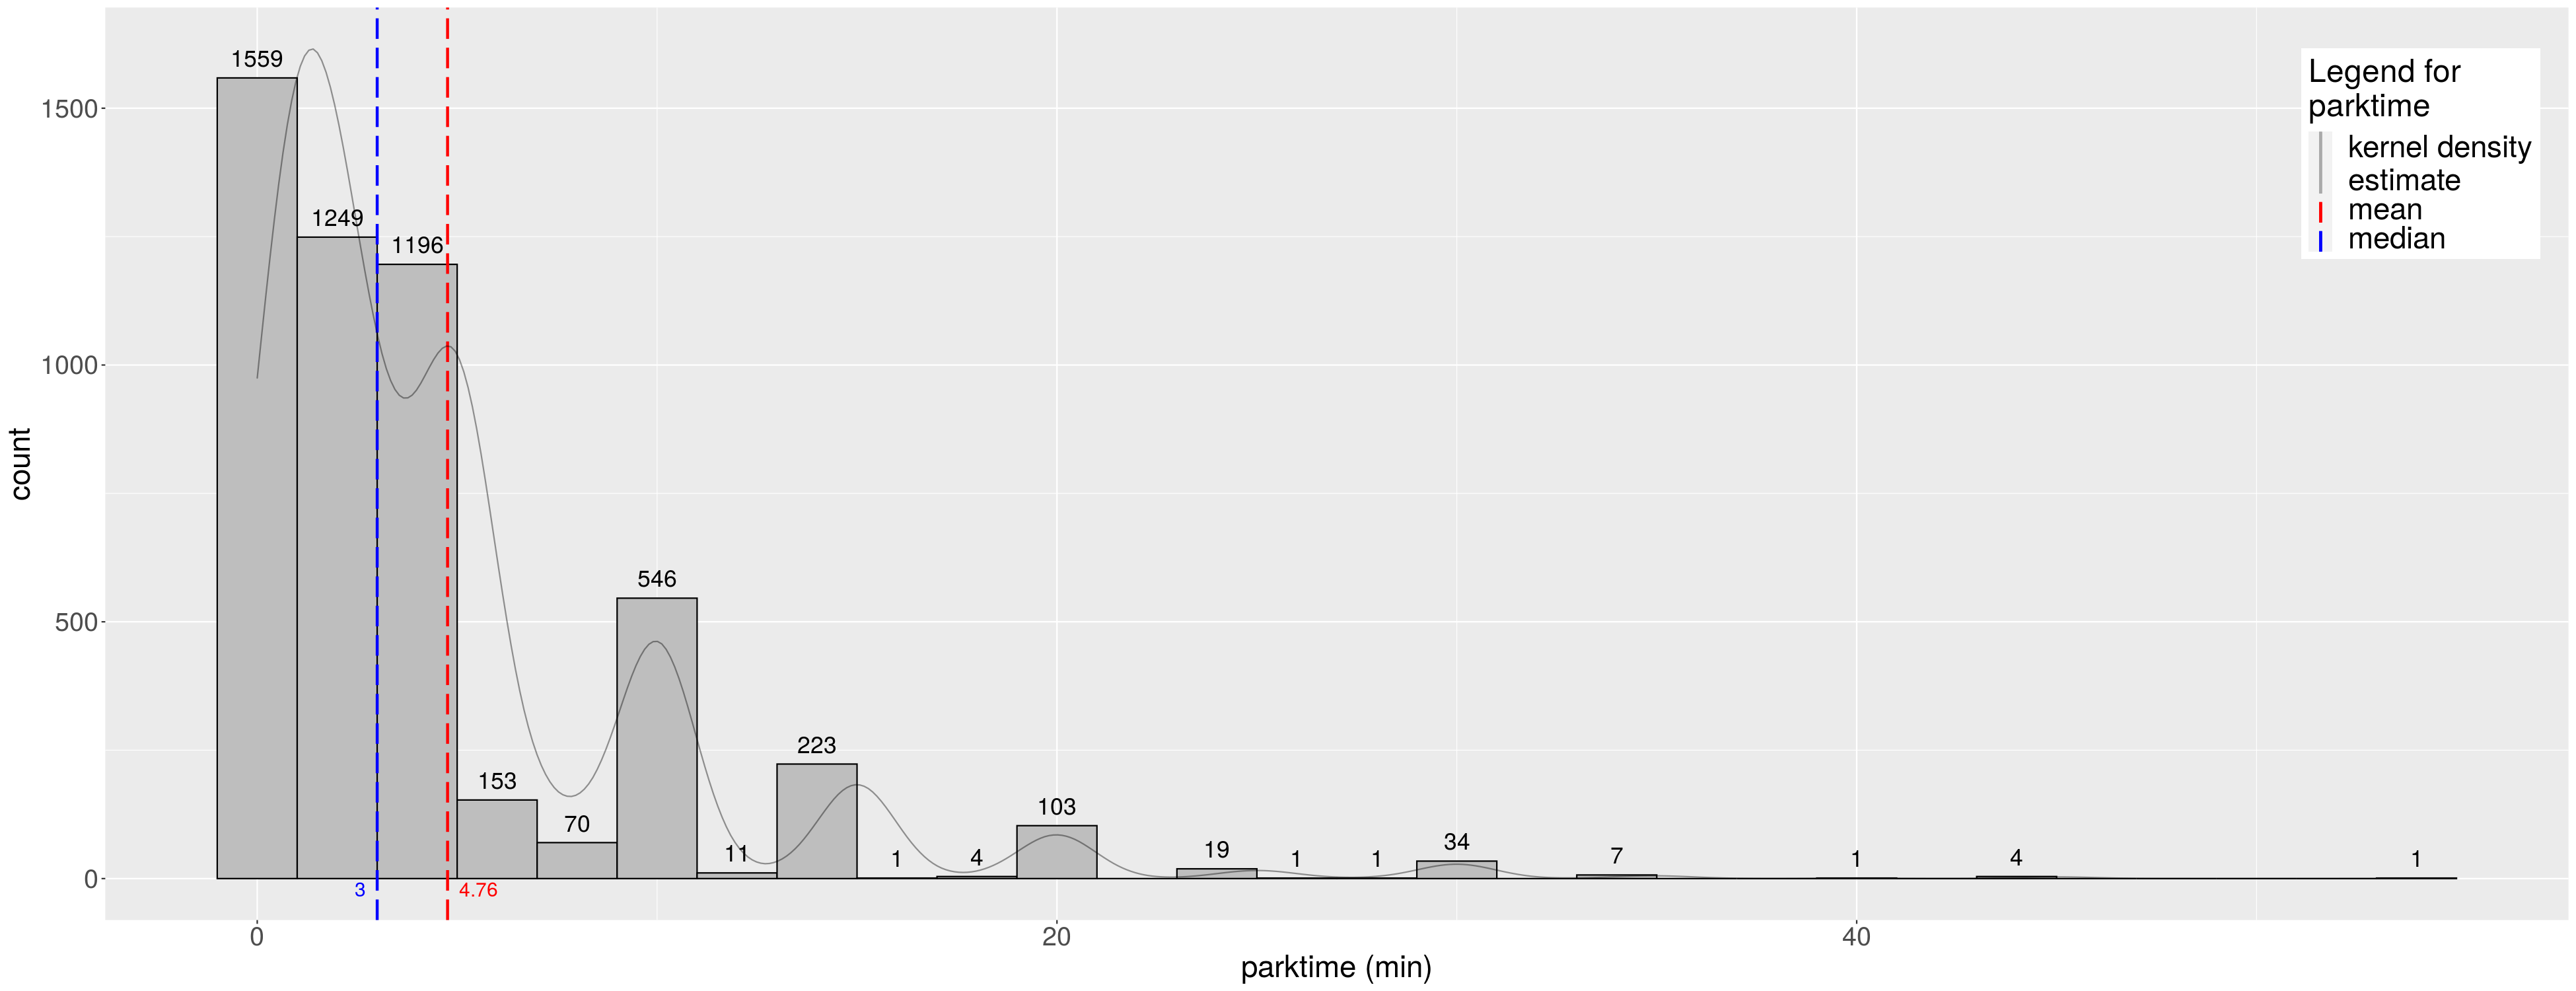
\includegraphics[width=\textwidth]{images/hist_pmax59-wmax59_parktime-likert_binw2_23-09-2020.png}
    \caption[Histogram, searching for parking]{All permitted thesis survey \code{parktime} values (< 60) shown on histogram. \textcolor{red}{larger text needed}}%
    \label{fig:parktime_hist}%
\end{figure}

\begin{figure}[H]%
    \centering
    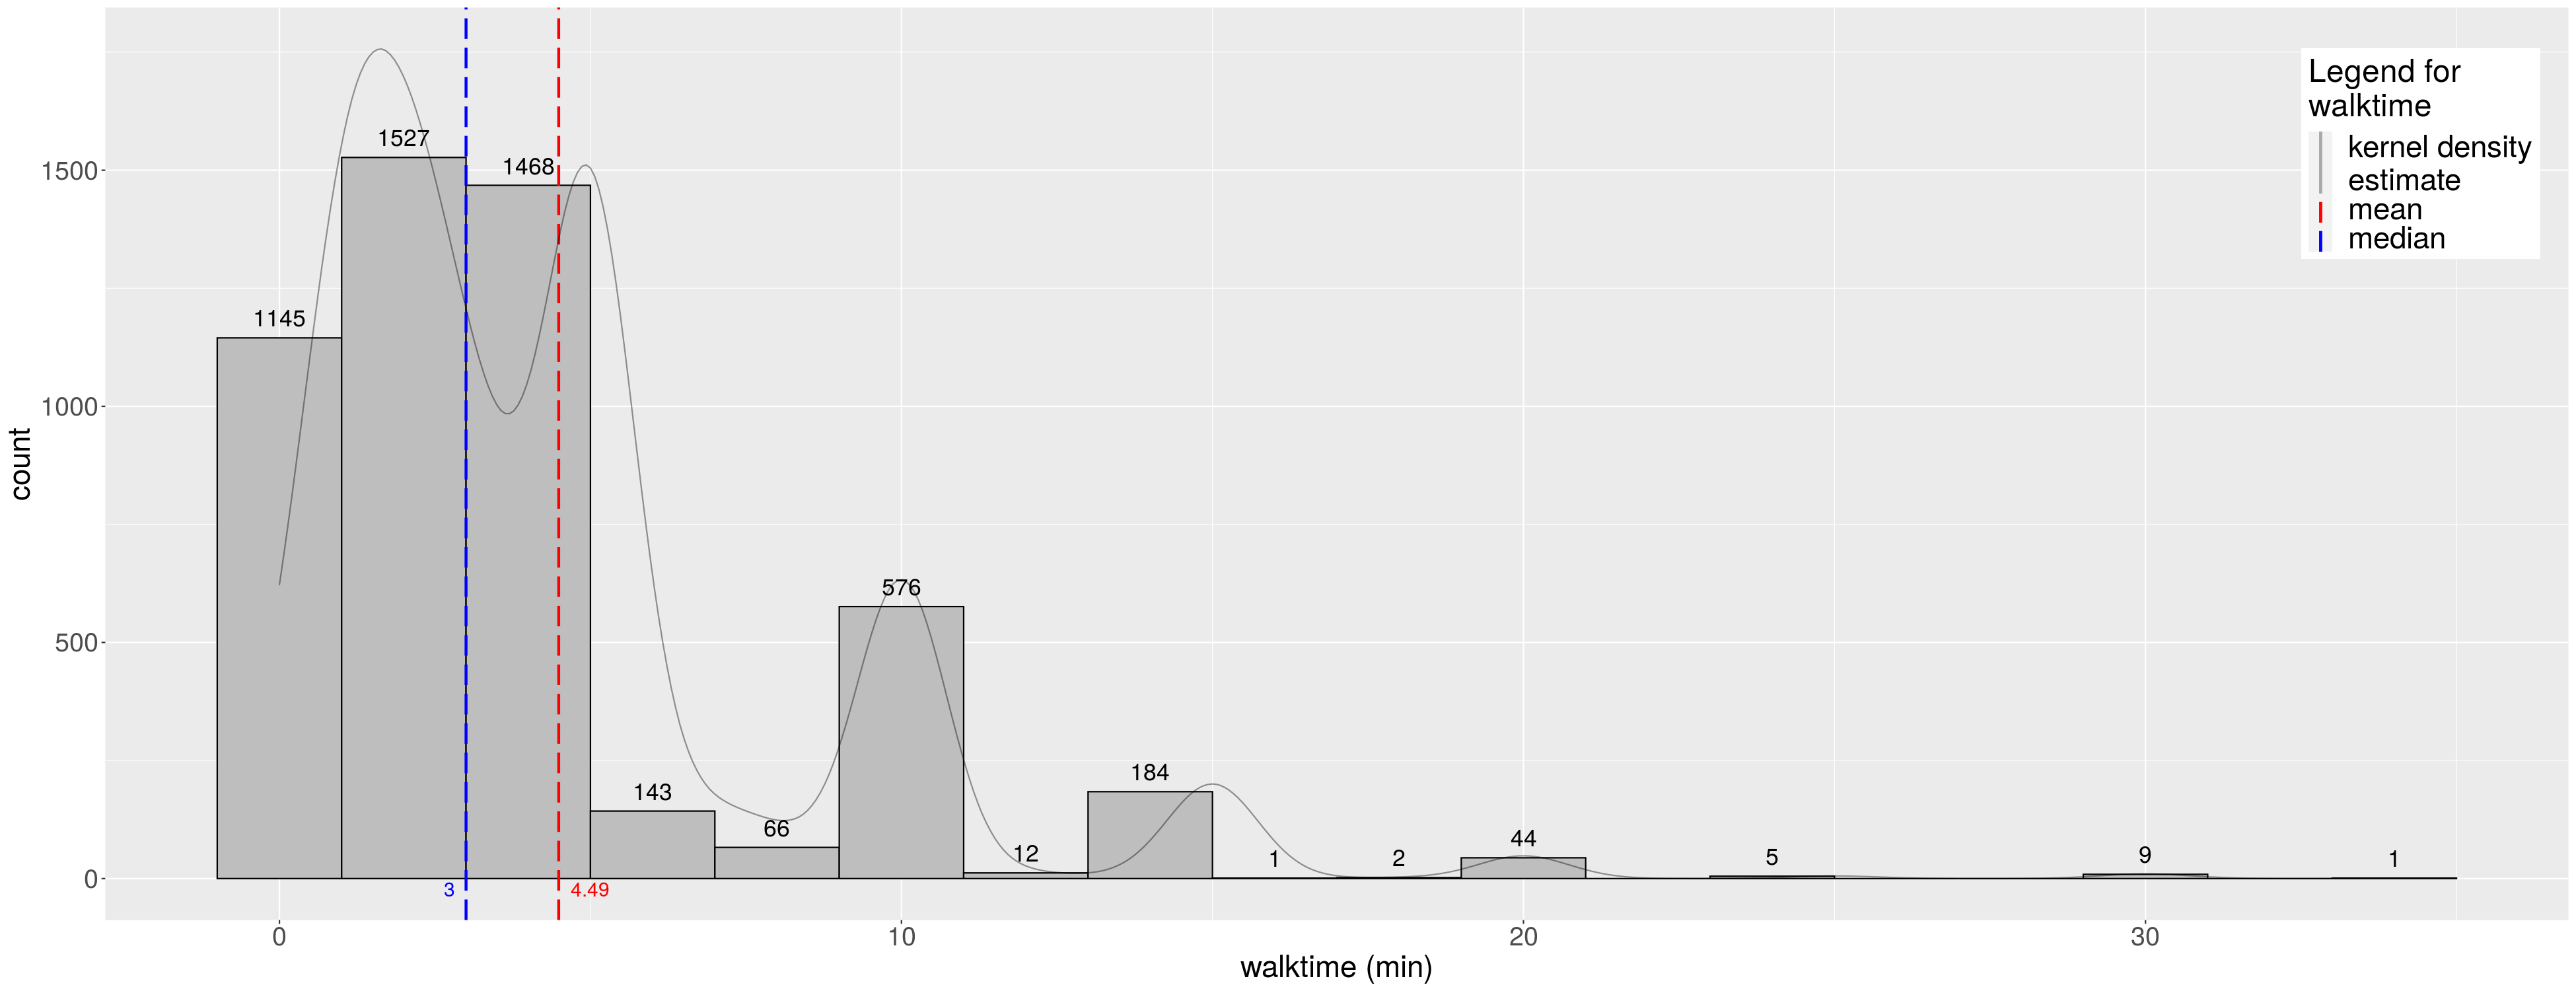
\includegraphics[width=\textwidth]{images/hist_pmax59-wmax59_walktime-likert_binw2_23-09-2020.png}
    \caption[Histogram, walk to destination]{All permitted thesis survey \code{walktime} values (< 60) shown on histogram. \textcolor{red}{larger text needed}}%
    \label{fig:walktime_hist}%
\end{figure}

On a closer look to the municipalities, finer details become apparent (figure~\ref{fig:postalvis_answers}). For example, in Helsinki, a wedge-like area of survey activity in the direction of southwest-northeast is visible. Starting out from the west, this area spans from Lauttasaari to the center of Helsinki and moving on all the way east to Malmi. Many of the areas which could be roughly characterised as residential areas were left with little activity. Furthermore, in the survey instructions respondents were requested to refrain from including parking activity in private property, as it was assumed in survey design phase that these areas would provide near to instantaneous parking, potentially distorting the data and obfuscating the objectives set by the thesis research questions. The lightness of activity in residential areas corresponds with the made request.

% A known issue with these maps: Vartiosaari is represented on these maps. As an unreachable island, it shouldn't.
\begin{figure}[H]%
    \centering
    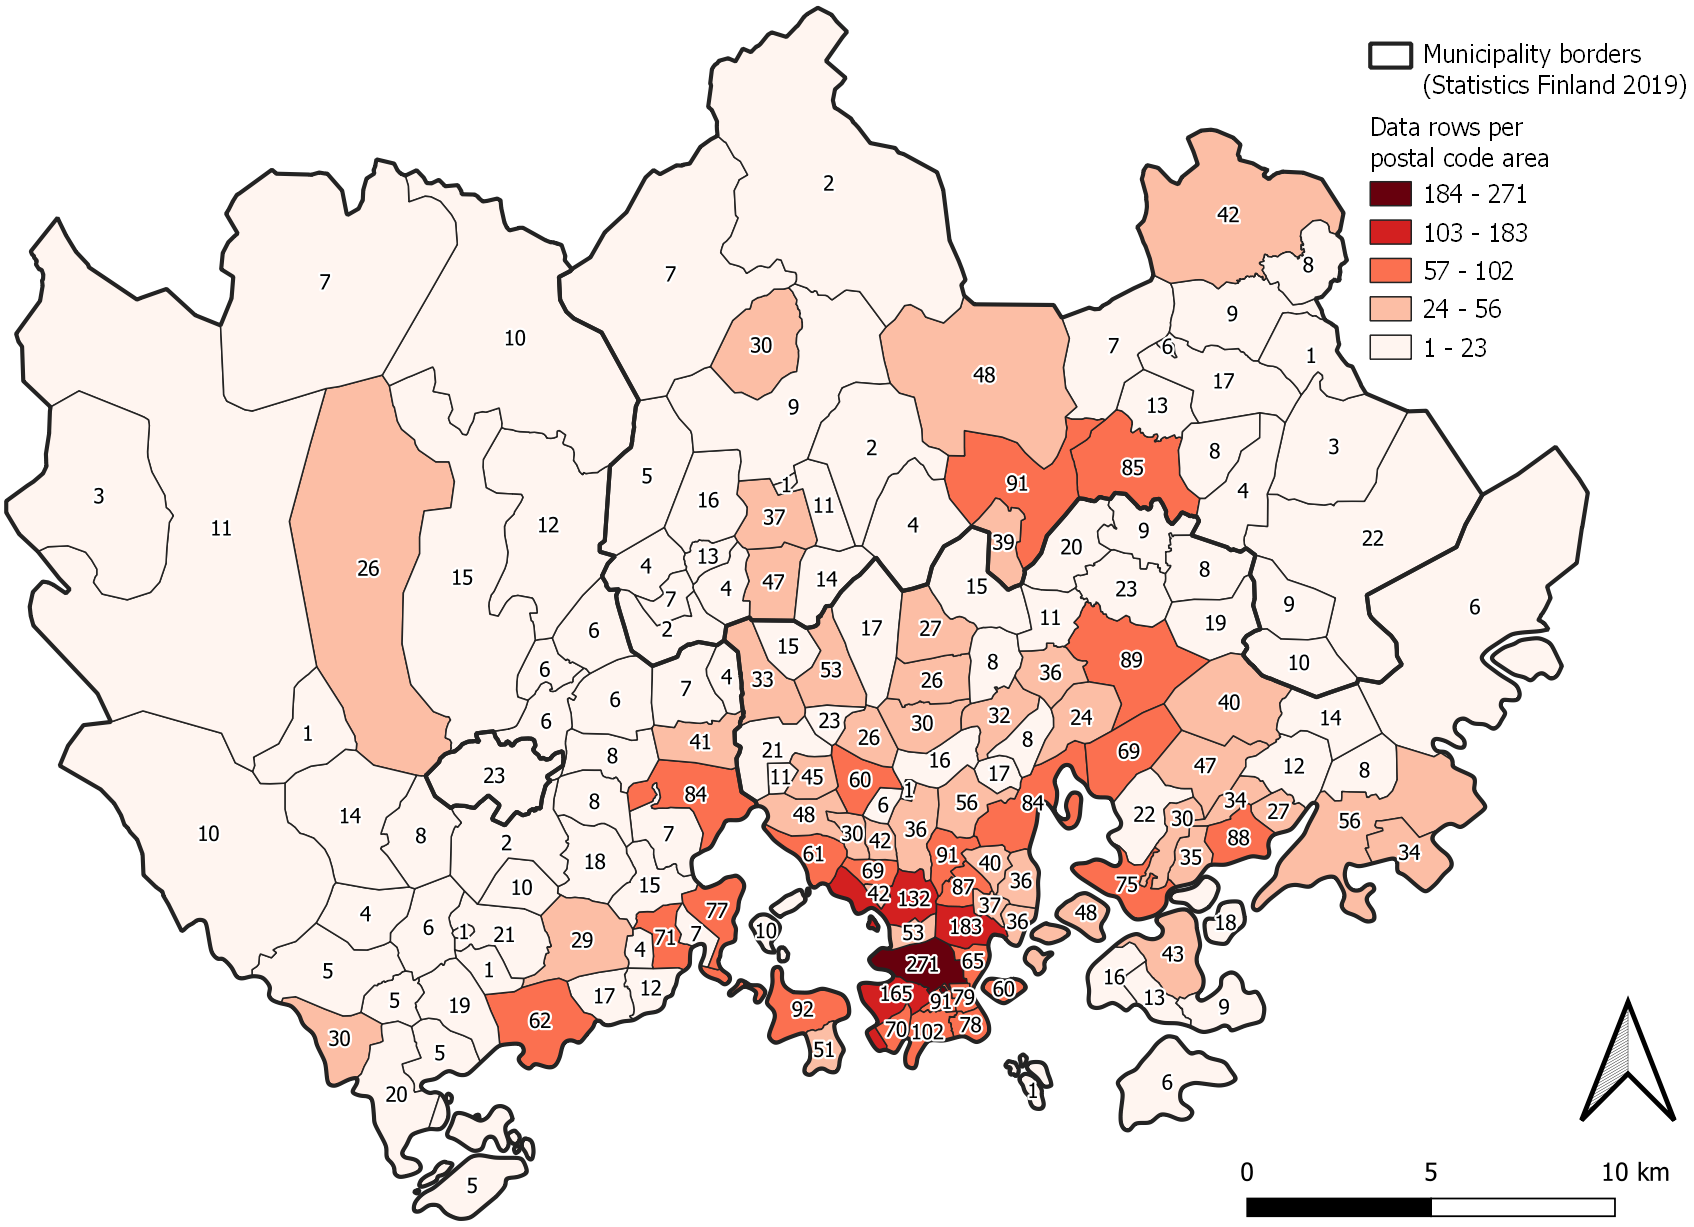
\includegraphics[width=\textwidth]{images/thesis_postalvis_answers.png}
    \caption[Data rows received per postal code area]{This figure illustrates the responses received in the thesis survey per postal code area (n=167). Classes are in natural breaks (Jenks). Municipality borders are based on \textit{postal} data. There are slight differences to the actual municipality boundaries. View these differences in figure~\ref{fig:thesis_resarea}.}%
    \label{fig:postalvis_answers}%
\end{figure}

In the finest resolution available, the postal code areas, long \code{parktime} values closely follow areas with most survey activity (figures~\ref{fig:postalvis_parkmean},~\ref{fig:postalvis_parkmedian}). The longest \code{parktime} values were encountered in the center of Helsinki, where the mean value for 00120 Punavuori was 10.6 minutes (median 10.0 minutes, 91 data rows) and 00290 Meilahden sairaala-alue 9.4 minutes (5.0 min, 42 rows). Long parking times over five minutes were recorded in all over the center area, but also in 00570 Kulosaari (5.3 min, 5.0 min, 48 rows) and 00590 Kaitalahti (6.5 min, 3.5 min, 16 rows). In Espoo, the longest \code{parktime} values were found in 02230 Matinkylä (5.1 min, 5.0 min, 62 rows), 02100 Tapiola (4.6 min, 3.0 min, 71 rows), and in 02320 Espoonlahti (4.3 min, 3.0 min, 30 rows). In Vantaa, it took the longest to find a parking spot in 01300 Tikkurila (6.4 min, 5.0 min, 85 rows). According to the survey results, it was relatively hard to find a parking spot in 01700 Kivistö (5.7 min, 4.0 min, 30 rows), too.

In the case of this survey dataset it is important to not lose sight of median, as mean is susceptible to outliers, of which there are many present. One such situation may be viewed in 01750 Keimola, where the mean \code{parktime} is 5.9 minutes, and median reads at 1.0 minute. In Keimola's situation, one respondent entered a \code{parktime} value of 25 minutes, severely skewing the total sample of seven values. It may be argued that when detecting areas of long duration of searching for parking, median is the better measure to identify areas of interest.

The descriptive \code{walktime} values follow the same municipal order as those of \code{parktime}: On average, in Helsinki it took 4.8 minutes (median 4.0 minutes) to walk from one's parked car to the final destination of the journey (figure~\ref{fig:postalvis_walkmean},~\ref{fig:postalvis_walkmedian}). In Vantaa, this process was 4.0 minutes (3.0 min), while Espoo had mean parking time of 3.9 minutes (2.0 min) and Kauniainen 2.2 minutes (2.0 min). Of the entire research area, Espoo's 02780 Kauklahti stood out with a mean walking time of 6.3 minutes (5.5 min) to one's destination. It is notable that this subdivision received 10 answers, ranking second to the last before Helsinki's 00890 Östersundom's total of 6 answers.

\textcolor{red}{overlap here vs subdiv totals of next chapter?}\\
When viewed through postal code areas, \code{walktime} shows the longest durations to walk from one's car to the final destination in Helsinki with the top belonging to 00100 Helsinki Keskusta -- Etu-Töölö (mean 7.4 minutes, median 5.0 minutes, 271 data rows). Most of the central Helsinki did not fall far behind with most values ranging from five to seven minutes. Outside of the center of Helsinki, 00570 Kulosaari (6.7 min, 5.0 min, 48 rows), 00590 Kaitalahti (6.3 min, 5.0 min, 16 rows) and 00690 Tuomarinkylä-Torpparinmäki (5.3 min, 3.0 min, 15 rows) saw long \code{walktime} values within the boundaries of Helsinki. Looking outward from the capital, the \code{walktime} values in Espoo were mostly lower than those in Helsinki. Longest recorded durations in Espoo were in 02100 Tapiola (5.4 min, 5.0 min, 71 rows), 02780 Kauklahti (6.3 min, 5.5 min, 10 rows), and 02820 Nupuri-Nuuksio (7.0 min, 5.0 min, 7 rows). Vantaa's longest \code{walktime} values were found in 01530 Veromiehenkylä (8.0 min, 5.5 min, 48 rows), 01300 Tikkurila (6.3 min, 5.0 min, 85 rows), and 01700 Kivistö (5.6 min, 5.0 min, 30 rows). 

It is difficult to try and determine the causes behind these long \code{walktime} values, but it may be worth noting, that many of the postal code areas with top values contain popular sightseeing locations, such as the Haltiala domestic animal farm in 00690 Tuomarinkylä-Torpparinmäki and the national park of Nuuksio in 02820 Nupuri-Nuuksio. The postal code area of 01530 Veromiehenkylä is almost entirely in the use of Helsinki-Vantaa Airport. It quickly becomes apparent that recreational trips to Nuuksio National Park may nudge the Espoo's \code{walktime} values upward, while in Vantaa, the Helsinki-Vantaa Airport walking seems to be a similar factor. A summarising feature about \code{walktime} is that areas of long walking times from one's car to the final destination are not as apparently clustered as those of \code{parktime} are.


\begin{figure}[H]%
    \centering
    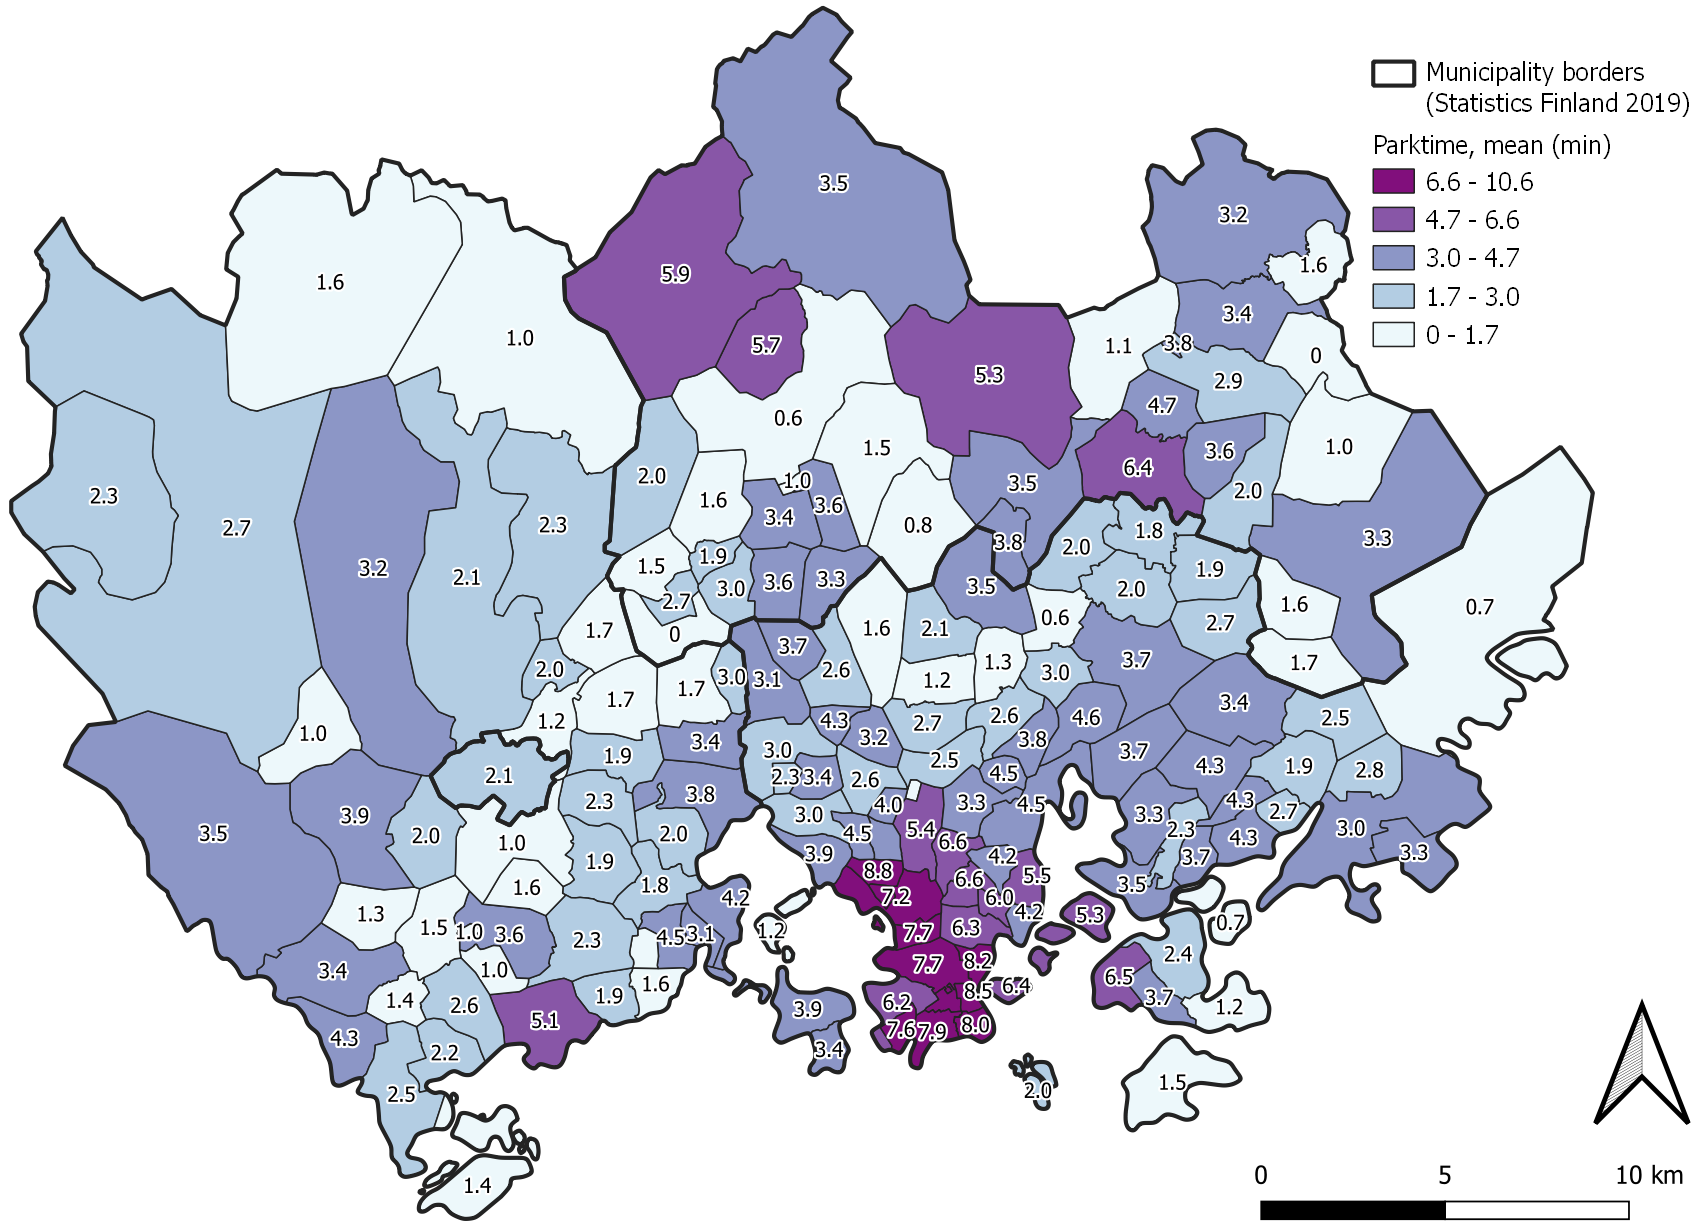
\includegraphics[width=\textwidth]{images/thesis_postalvis_parkmean.png}
    \caption[Parktime, mean, in the reseach area]{This figure illustrates the mean duration of searching for parking and parking one's car in each postal code area.}%
    \label{fig:postalvis_parkmean}%
\end{figure}

\begin{figure}[H]%
    \centering
    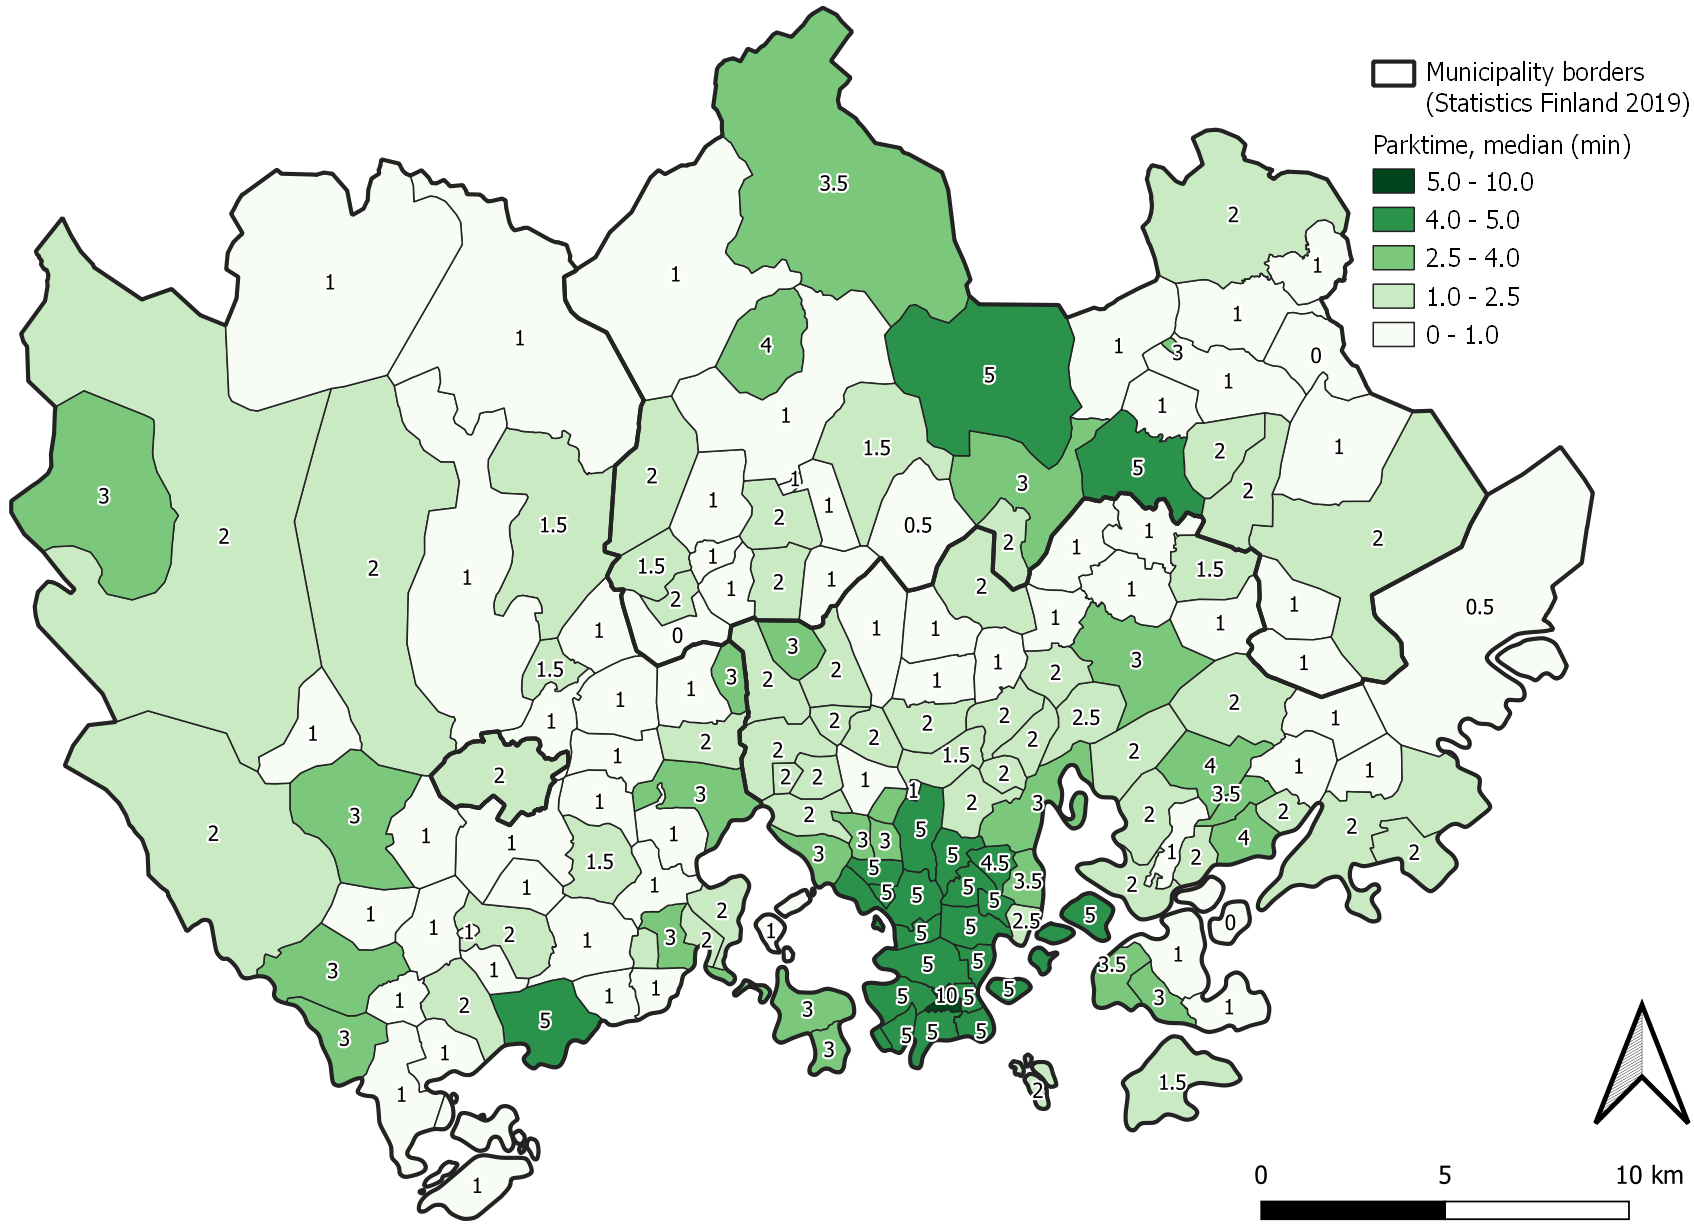
\includegraphics[width=\textwidth]{images/thesis_postalvis_parkmedian.png}
    \caption[Parktime, median, in the reseach area]{This figure illustrates the median duration of searching for parking and parking one's car in each postal code area.}%
    \label{fig:postalvis_parkmedian}%
\end{figure}

\begin{figure}[H]%
    \centering
    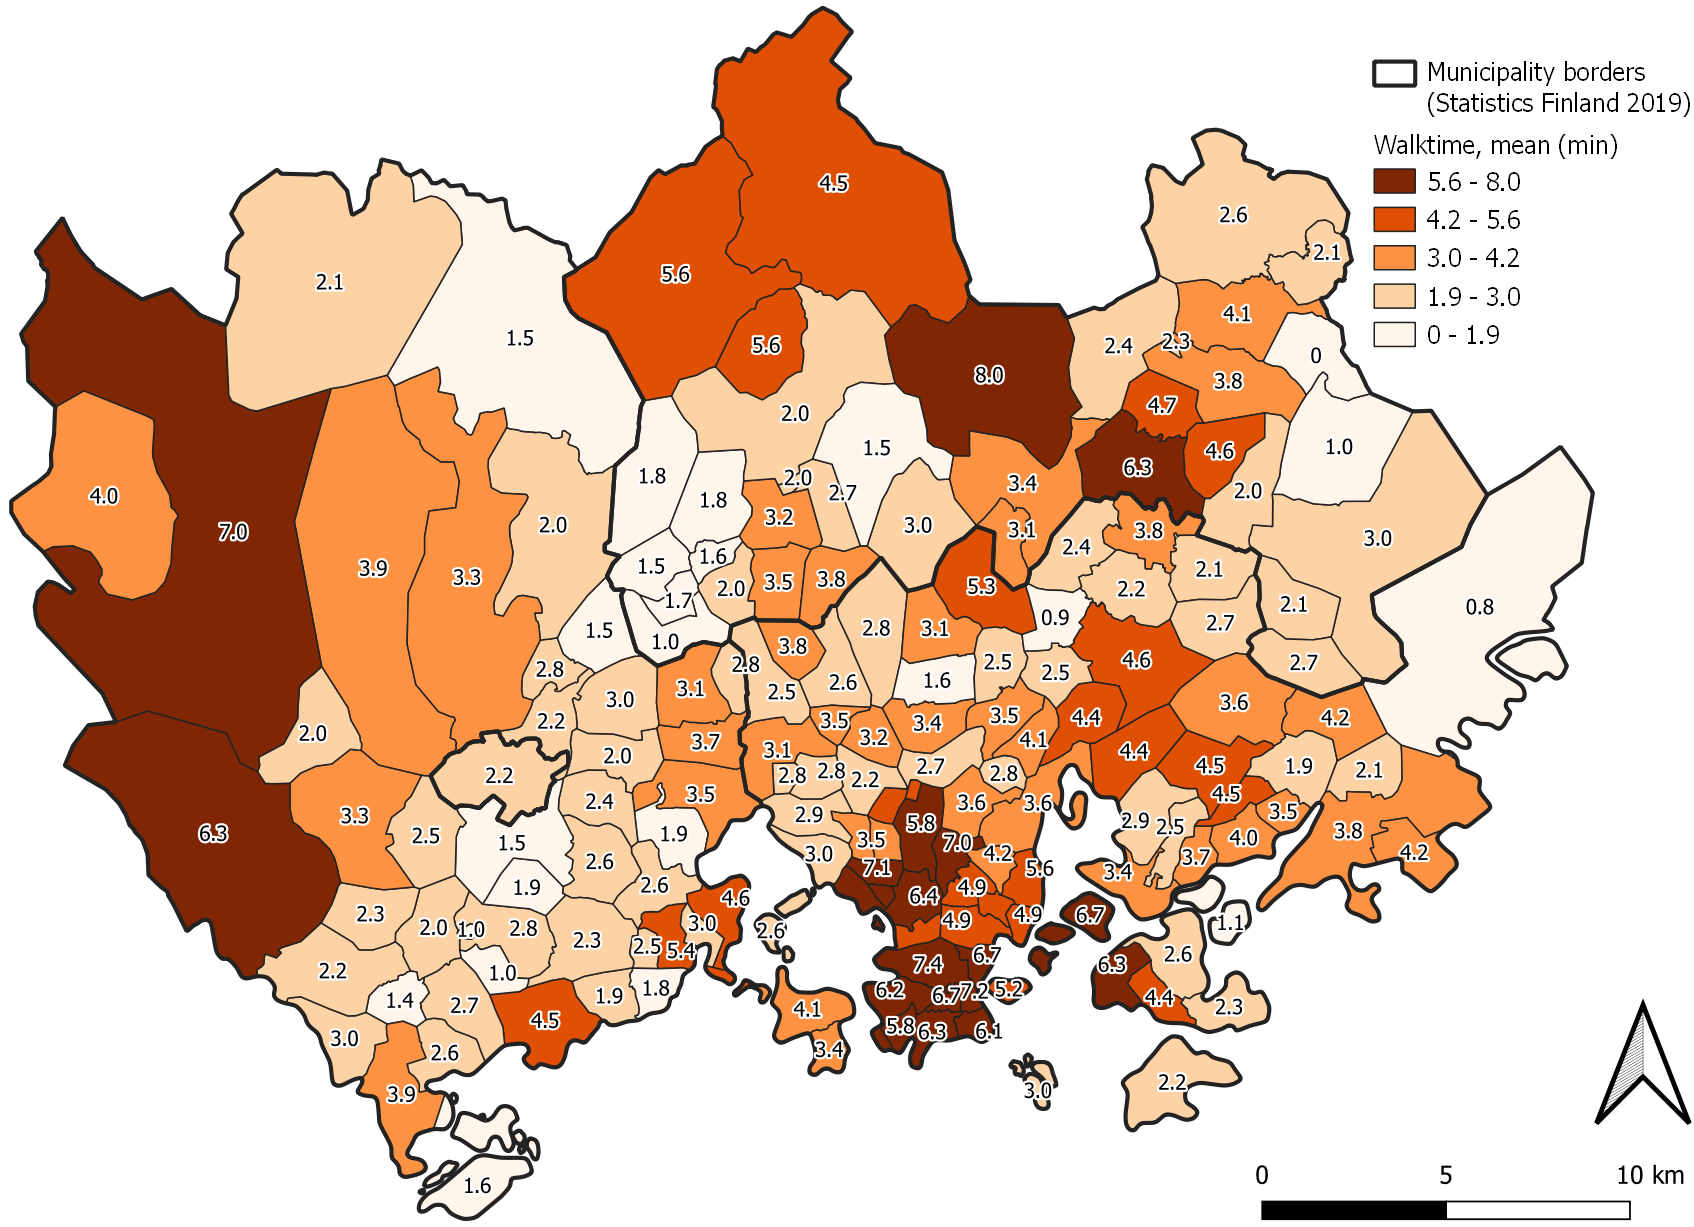
\includegraphics[width=\textwidth]{images/thesis_postalvis_walkmean.png}
    \caption[Walktime, mean, in the research area]{This figure illustrates the mean duration of walking from one's parked car to the final destination in each postal code area.}%
    \label{fig:postalvis_walkmean}%
\end{figure}

\begin{figure}[H]%
    \centering
    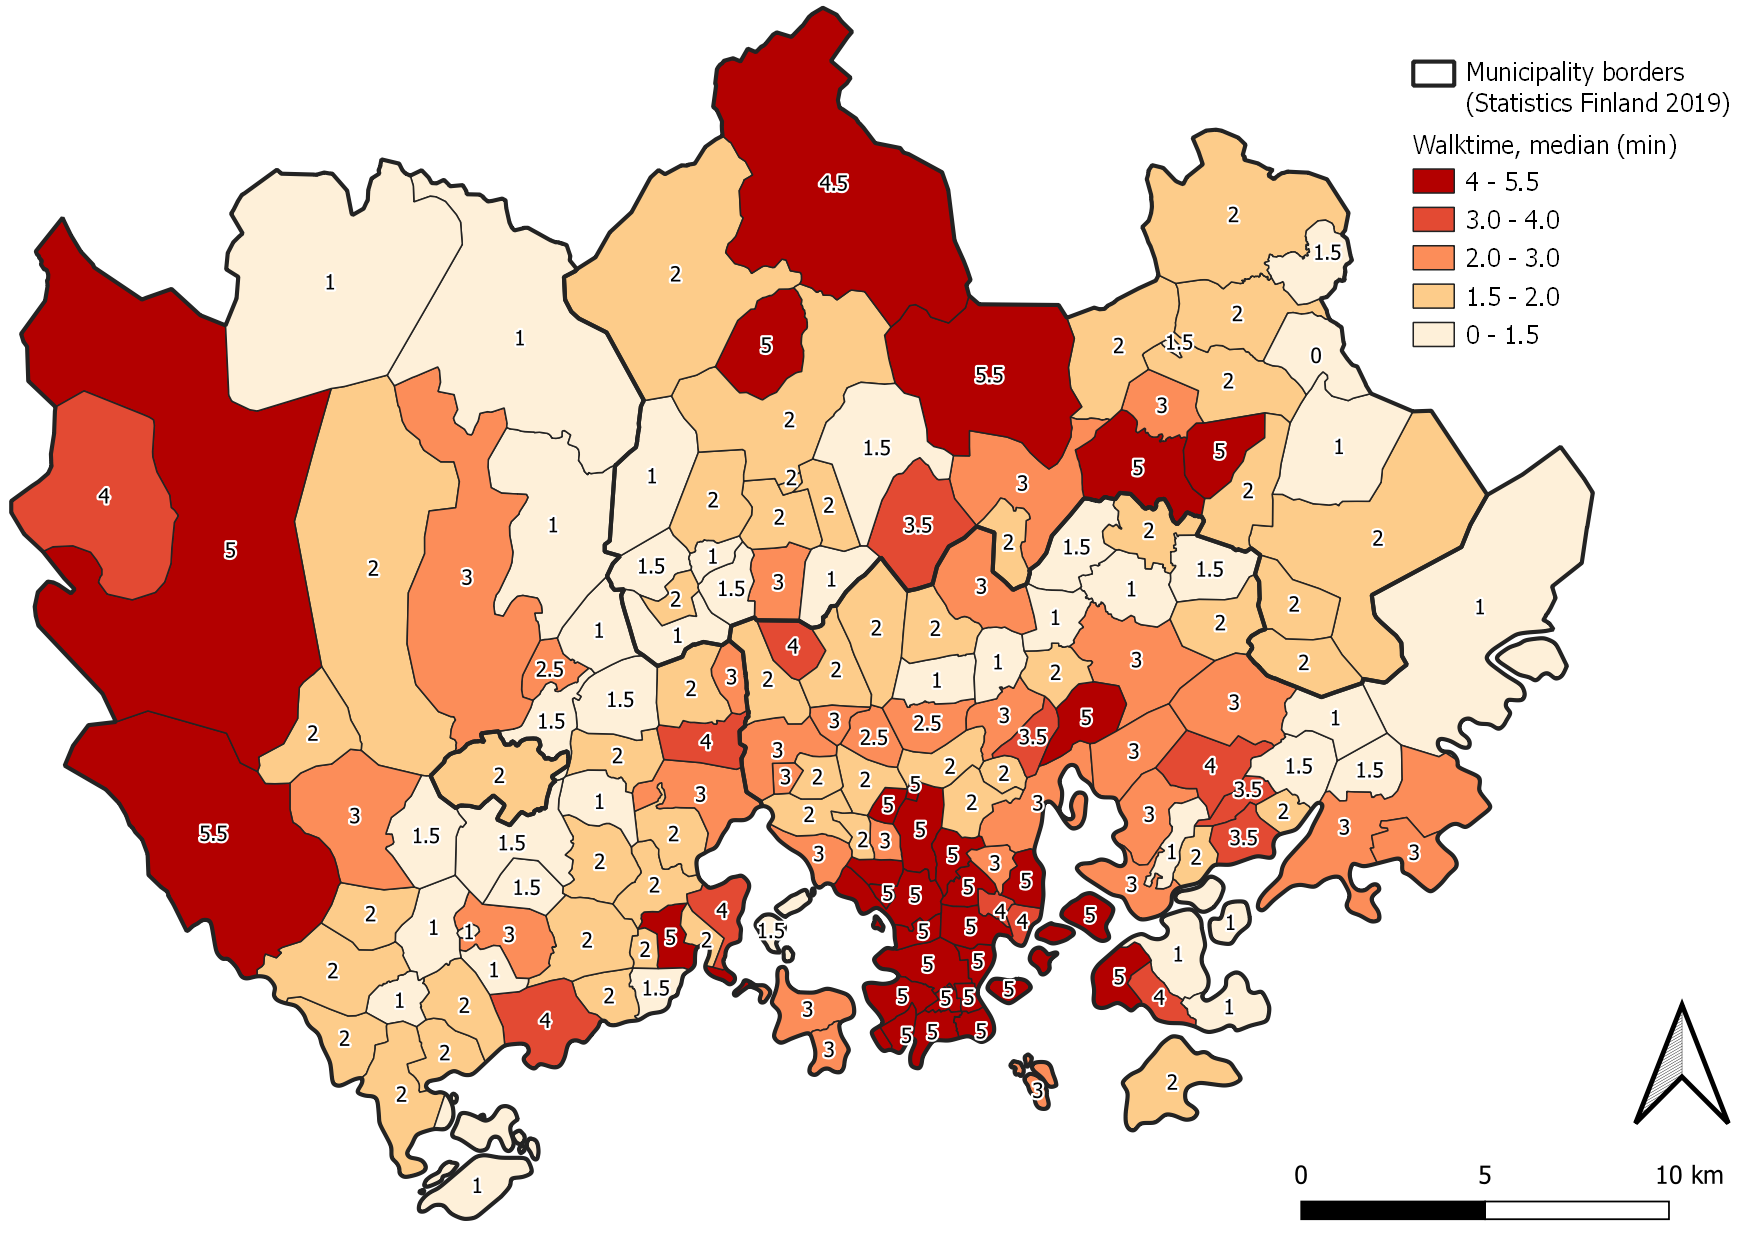
\includegraphics[width=\textwidth]{images/thesis_postalvis_walkmedian.png}
    \caption[Walktime, median, in the research area]{This figure illustrates the median duration of walking from one's parked car to the final destination in each postal code area.}%
    \label{fig:postalvis_walkmedian}%
\end{figure}

\newpage
\subsection{Explanatory data analysis}
\justify

%https://www.thoughtco.com/population-vs-sample-standard-deviations-3126372
%--- ilmeisesti sample standard deviation on yleisesti parempi kuin population! ja ehkäpä mun aineisto on useammin sample kuin koko population, joten voinen unohtaa tuon!
%https://towardsdatascience.com/understanding-descriptive-statistics-c9c2b0641291
%https://towardsdatascience.com/understanding-boxplots-5e2df7bcbd51
%https://towardsdatascience.com/analysis-of-variance-and-its-variations-6ef3f8fbeb05

% tärkeää, lisää f statisticit!
% https://www.statisticshowto.com/probability-and-statistics/f-statistic-value-test/#FandP
\textcolor{red}{ANOVA normality assumed through central limit theorem, expand on this} \\
The thesis survey data reveals that there are spatial differences between municipalities and regions of Helsinki Capital Region (table~\ref{tab:park_walk_subdiv}) in the durations to find a parking spot (\code{parktime}), and walking from one's parked car to the final destination (\code{walktime}). This is shown by the one-way \acrfull{anova} that for \code{parktime} and \code{walktime} there are statistically significant differences ($p < 0.05$) between the 23 groups (municipality subdivisions, figure~\ref{fig:subdiv_placement}). In the vast majority of subdivision groups, the group sizes were sufficiently large for \acrshort{anova} analysis to be highly significant ($p < 0.001$). An exception to this is the \acrshort{anova} test for Espoo's subdivisions using \code{parktime}. This test finishes with a less significant $p = 0.015$.

The spatial differences between subdivisions were wide-ranging, with a 5.2 minutes mean (median 4.0 minutes) \code{parktime} in Helsinki, 3.8 minutes in Vantaa (2.0 min), 3.2 minutes in Espoo (2.0 min) and lastly, 2.1 minutes (2.0 min) in Kauniainen. Durations to find a parking spot varied inside municipalities; in Espoo, in the subdivision of Pohjois-Espoo mean \code{parktime} was 1.7 minutes (1.0 min) while the same value for Suur-Matinkylä was 4.3 minutes (3.0 min). From all the subdivisions in the research area, the subdivision representing the center of Helsinki, Helsinki Southern, had the the longest mean \code{parktime}, 7.3 minutes (5.0 min). Kauniainen ranked as fourth with a \code{parktime} values 2.1 minutes mean (2.0 min).

Viewing \code{walktime} through subdivisions, longest \code{walktime} was found from Espoo's Suur-Kauklahti (mean 6.3 min, median 5.5 min). In Helsinki, the Southern subdivision's durations were the second longest (mean 6.3 min, median 5.0 min) with Vantaa's top values reaching 5.8 minutes mean and 5.0 median in Tikkurila. Kauniainen's \code{walktime} values were more moderate with 2.2 minutes mean and 2.0 minutes median.

When comparing specific subdivisions, we can observe finer details in the survey dataset. For example, comparing \code{parktime} in Espoo's Suur-Tapiola and Vantaa's Aviapolis gives no statistical significance with \acrshort{anova} ($p = 0.121$). However, a test with Suur-Tapiola and Helsinki's Southern subdivision is statistically significant ($p < 0.001$). It is interesting, that an \acrshort{anova} \code{parktime} comparison of Espoo's Suur-Leppävaara and Helsinki's Northeastern subdivisions -- both important subcenters of their respective cities -- produces no statistical significance ($p = 0.850$). 

Differences of Espoo's Vanha-Espoo and Helsinki's Östersundom subdivisions viewed with \code{walktime} gives a faint statistical significance with \acrshort{anova} ('.', $p = 0.054$). Testing areas with contrasting features, Vanha-Espoo and Vantaa's Tikkurila proved statistically significant ('**', $p = 0.004$). It is interesting that important city centers receive different results from the \acrshort{anova} test. For example, differences in \code{walktime} are statistically significant (’***’, $p \leq 0.001$) between Vantaa's Myyrmäki and Tikkurila subdivisions. \code{walktime} differences of Espoo's Suur-Matinkylä and Suur-Leppävaara are not ('$ns$', $p = 0.132$). The same case stands for Helsinki's Southeastern and Western subdivisions of which differences were not identified as statistically significant ('$ns$', $p = 0.762$). However, varying degrees of significance is found for the same subdivision comparison pairs when using \code{parktime} as the explanatory variable: Myyrmäki--Tikkurila achieves high statistical significance (’***’, $p \leq 0.001$), while Suur-Matinkylä--Suur-Leppävaara ('**', $p = 0.007$), and Southeastern--Western ('**', $p = 0.007$) get moderate significance.

% 290720 kun verrataan kahta subdiviä (2 ryhmää), käytetään anovaa ja katsotaan merkitsevyys. Suur-Tapiola ja Aviapolis oli " ", ei-merkitsevä, Suur-Tapiola ja Helsinki Southern ***. Kirjoita muutamasta parista, joissa ***. Vois mainita yhden kiinnostavan, missä parkkiaikojen ero on kohinaa (Tapiola ja Aviapolis). Muista tää sama walktimelle. \\
% 290720 katso muut muuttujat niin, että mukana kaikki subdivit, onko merkitsevyyttä anovassa \\
% 290720 parktime: verrataan arki-viikonloppu, **, walktime: ei ole ollenkaan! \\
% voi tutkii myös kaupunkien erot pareina, mutta tämä taitaa tarvita koodia \\
% parktime Espoossa ja Helsingissä (eri tarkastelut), espoossa ei niin väliä milloin pysäköi, kun taas helsingissä merkittävämmät erot \\
% 290720 vantaan timeofday arkiruuhka ja arkiei-ruuhka oudot tulokset, arkiruuhka nopeampi. Mutta tämä on ei-merkitsevä anovan mukaan!
% 290720 espoon timeofdayn pienet erot ovat kohinaa anovan mukaan (ei-merkitsevä), can't specify ei mukana
% 290720 anova kertoo että onks vähintään JOKU 1 ryhmä merkitsevästi eri kuin muut, sitten seuraavaksi pitäis tutkii lisää, vaikka pareittain

%https://www.researchgate.net/post/Is_there_a_minimum_number_per_group_neccessary_for_an_ANOVA
%anova - ryhmän koko anovassa
% interpret anova table in r
%http://www.understandingdata.net/2017/05/11/anova-tables-in-r/
%https://www.statisticssolutions.com/sample-size-calculation-for-one-way-anovas-in-dissertations-and-theses/

% levene näyttää vain vähän eri, niin ei oo välii, sitten pitäis kattoo keskihajontaa
%anova pitäis olla ok koska 20 tapausta jo riittävä tuloksen löytymiseen 
%voin todeta, että on tilastolliseti merkitsevä ero, sitten vaan raportoi mikä on ero, esim espoo vs helsinki
%anova todistaa, että kaikilla esim "subdiveillä" ei ole samoja arvoja
%-- parittaiset t-testit jos haluaa kahden paikan välillä testailla
%-- viikonloppuaikojen sisällä varianssi ja viikonpäivän varianssi, kuinka paljon varianssista se selittää
%-- power-analyysi?? Eta-squared (eta2)

%https://statistics.laerd.com/spss-tutorials/one-way-anova-using-spss-statistics-2.php
%LINKISTÄ: therefore, there is a statistically significant difference in the
%mean length of time to complete the spreadsheet problem between the different 
%courses taken.
\begin{hyphenrules}{nohyphenation}
    \begin{table}[H]
        \centering
        \caption[Parktime and walktime descriptive statistics with explanatory variable subdiv]{Parking times and walking times descriptive statistics displayed by municipalities and subdivisions (the explanatory variable \code{subdiv}). The unit of median, mean, and standard deviation is minutes. The f value and p value presented are calculated in One-way \acrfull{anova}. P value significance codes: '***' $p \leq 0.001$, '**' $p \leq 0.01$, '*' $p \leq 0.05$, '.' $p \leq 0.1$, 'ns' $p \leq 1$.}
        \label{tab:park_walk_subdiv}
        \scalebox{0.66}
        % Column type C is a custom column which adds space to its position. Used to separate important features of this table. L aligns left.
        {\begin{tabular}{clLccccCcccccc}
            \toprule
		    & & &                                       \multicolumn{5}{c}{parktime} &          \multicolumn{5}{c}{walktime} \\
														\cmidrule(lr{\tbspace}){4-8}            \cmidrule(lr){9-13}
            \multirow{2}{*}{} & \multirow{2}{*}{} & \multirow{2}{*}{n} & \multirow{2}{*}{Median} & \multirow{2}{*}{Mean} & \multirow{2}{*}{Std.dev} & \multirow{2}{*}{Std.err} & f value, & \multirow{2}{*}{Median} & \multirow{2}{*}{Mean} & \multirow{2}{*}{Std.dev} & \multirow{2}{*}{Std.err} & f value, \\
            & & & & & & & p value & & & & & p value \\
            
            \midrule
            \multirow{7}{*}{Espoo} & Pohjois-Espoo &    29 & 1 & 1.69 & 2.12 & 0.39 & &         1 & 1.86 & 1.55 & 0.29 & \\
            & Suur-Espoonlahti &                        99 & 2 & 2.88 & 3.27 & 0.33 & &         2 & 2.83 & 2.67 & 0.27 & \\
            & Suur-Kauklahti &                          10 & 2 & 3.50 & 3.69 & 1.17 & &         5.5 & 6.30 & 4.81 & 1.52 & \\
            & Suur-Leppävaara &                         176 & 2 & 3.12 & 2.94 & 0.22 & &        3 & 3.27 & 2.41 & 0.18 & \\
            & Suur-Matinkylä &                          95 & 3 & 4.28 & 4.05 & 0.42 & &         3 & 3.76 & 2.81 & 0.29 & \\
            & Suur-Tapiola &                            257 & 2 & 3.33 & 3.94 & 0.25 & &        2 & 3.84 & 3.41 & 0.21 & \\
            & Vanha-Espoo &                             80 & 2 & 2.81 & 4.00 & 0.45 & &         3 & 3.89 & 3.81 & 0.43 & \\
            % Use \arrayrulecolor to get a grey cmidrule, then revert \midrule color back to black
            \arrayrulecolor{black!30}\cmidrule(lr){2-13}
            \multirow{2}{*}{} & \multirow{2}{*}{\textbf{Total}} & \multirow{2}{*}{746} & \multirow{2}{*}{2} & \multirow{2}{*}{3.23} & \multirow{2}{*}{3.63} & \multirow{2}{*}{0.13} & value, & \multirow{2}{*}{2} & \multirow{2}{*}{3.52} & \multirow{2}{*}{3.09} & \multirow{2}{*}{0.11} & value, \\
            & & & & & & & 0.015 (*) & & & & & < 0.001 (***) \\
            \arrayrulecolor{black}\midrule
            
            \multirow{8}{*}{Helsinki} & Central &       704 & 5 & 5.54 & 5.72 & 0.22 & &        5 & 4.91 & 3.92 & 0.15 & \\
            & Eastern &                                 360 & 2 & 3.61 & 3.41 & 0.18 & &        3 & 3.91 & 3.51 & 0.18 & \\
            & Northeastern &                            308 & 2 & 3.19 & 3.83 & 0.22 & &        3 & 3.63 & 3.47 & 0.20 & \\
            & Northern &                                162 & 1 & 2.38 & 2.73 & 0.21 & &        2 & 3.16 & 3.21 & 0.25 & \\
            & Southeastern &                            315 & 2 & 3.42 & 3.72 & 0.21 & &        2 & 3.70 & 3.79 & 0.21 & \\
            & Southern &	                            1310 & 5 & 7.26 & 6.47 & 0.18 & &       5 & 6.23 & 4.56 & 0.13 & \\
            & Western &                                 612 & 2 & 4.28 & 5.04 & 0.20 & &        3 & 3.63 & 3.15 & 0.13 & \\
            & Östersundom &                             6 & 0.5 & 0.67 & 0.82 & 0.33 & &        1 & 0.83 & 0.75 & 0.31 & \\
            \arrayrulecolor{black!30}\cmidrule(lr){2-13}
            \multirow{2}{*}{} & \multirow{2}{*}{\textbf{Total}} & \multirow{2}{*}{3777} & \multirow{2}{*}{4} & \multirow{2}{*}{5.24} & \multirow{2}{*}{5.60} & \multirow{2}{*}{0.09} & value, & \multirow{2}{*}{4} & \multirow{2}{*}{4.78} & \multirow{2}{*}{4.10} & \multirow{2}{*}{0.07} & value, \\
            & & & & & & & < 0.001 (***) & & & & & < 0.001 (***) \\
            \arrayrulecolor{black}\midrule
            
            Kauniainen & Kauniainen &                   23 & 2 & 2.13 & 1.60 & 0.33 & --- &     2 & 2.22 & 1.28 & 0.27 & --- \\
            \midrule
            
            \multirow{7}{*}{Vantaa} & Aviapolis &       184 & 3 & 3.93 & 4.09 & 0.30 & &        3 & 4.51 & 4.27 & 0.31 & \\
            & Hakunila &                                44 & 1.5 & 2.41 & 2.89 & 0.44 & &       2 & 2.59 & 2.47 & 0.37 & \\
            & Kivistö &                                 48 & 1 & 4.69 & 6.37 & 0.92 & &         3 & 4.88 & 4.99 & 0.72 & \\
            & Koivukylä &                               40 & 1 & 2.80 & 3.74 & 0.59 & &         2 & 3.33 & 3.69 & 0.58 & \\
            & Korso &                                   50 & 2 & 2.92 & 4.43 & 0.63 & &         2 & 2.50 & 1.59 & 0.23 & \\
            & Myyrmäki &                                161 & 2 & 2.98 & 4.13 & 0.33 & &        2 & 2.83 & 3.08 & 0.24 & \\
            & Tikkurila &                               110 & 5 & 5.84 & 5.60 & 0.53 & &        5 & 5.85 & 5.15 & 0.49 & \\
            \arrayrulecolor{black!30}\cmidrule(lr){2-13}
            \multirow{2}{*}{} & \multirow{2}{*}{\textbf{Total}} & \multirow{2}{*}{637} & \multirow{2}{*}{2} & \multirow{2}{*}{3.82} & \multirow{2}{*}{4.65} & \multirow{2}{*}{0.18} & value, & \multirow{2}{*}{3} & \multirow{2}{*}{3.98} & \multirow{2}{*}{4.11} & \multirow{2}{*}{0.16} & < value, \\
            & & & & & & & < 0.001 (***) & & & & & < 0.001 (***) \\
            \arrayrulecolor{black}\midrule
            
            \multirow{2}{*}{All} & \multirow{2}{*}{\textbf{Total}} & \multirow{2}{*}{5183} & \multirow{2}{*}{3} & \multirow{2}{*}{4.76} & \multirow{2}{*}{5.29} & \multirow{2}{*}{0.07} & value, & \multirow{2}{*}{3} & \multirow{2}{*}{4.49} & \multirow{2}{*}{3.99} & \multirow{2}{*}{0.06} & value, \\
            & & & & & & & < 0.001 (***) & & & & & < 0.001 (***) \\
            \bottomrule
        \end{tabular}}
    \end{table}
\end{hyphenrules}

The municipalities of Helsinki Capital Region show varying results when \code{parktime} and \code{walktime} were viewed against the thesis survey variable \code{timeofday}, the time of day for parking one's car (table~\ref{tab:park_walk_timeofday}). Highest values for each choice were found in Helsinki, where \code{parktime} mean was highest for \textit{Weekday, rush hour} (mean 5.7 min, median 5.0 min). Interestingly, none of the other municipalities had \textit{Weekday, rush hour} as the longest choice. In Espoo the choice \textit{Can't specify, no usual time} was the longest (3.8 min, 2.0 min), while in Vantaa the choice \textit{Weekday, other than rush hour} took the top position (4.2 min, 2.0 min). In Kauniainen survey participants reported the longest \code{parktime} values during the weekend (3.0 min, 3.0 min).

Furthermore, Helsinki also had the longest \code{walktime} values when viewed against \code{timeofday}. In the capital it took the longest to walk from one's car to the final destination on weekend (mean 5.1 min, median 5.0 min). For Espoo, survey participants again reported the highest \code{walktime} value for the choice \textit{Can't specify, no usual time} (4.0 min, 3.0 min). In Vantaa one had to walk the longest from the car to the final destination during weekday's rush hour (4.7 min, 3.0 min), while in Kauniainen weekend private car users spent the longest time walking from their car to their destination (2.6 min, 2.0 min).

The one-way \acrshort{anova} test yielded varying results when comparing choices of \code{timeofday} inside municipalities of Helsinki Capital Region. Highly significant differences between the time of day of parking and walking from one's car to the final destination were only detected in Helsinki, where both \code{parktime} and \code{walktime} received significance of $p \leq 0.001$. The corresponding test for Espoo produced a weaker statistical significance with \code{parktime} ('*', $p = 0.04$) and \code{walktime} ('*', $p = 0.02$). The \acrshort{anova} tests were entirely non-significant while Vantaa's \acrshort{anova} test testing \code{timeofday} produced a non-significant result for \code{parktime} and a weak significance for \code{walktime} ('.', $p = 0.07$).

Groups were excluded from the variable \code{timeofday} in a test to see if it would enhance statistical significance of differences between the rest of the groups. This proved unsuccessful. For example, statistically significant differences could not be found for \code{timeofday} groups when concentrating on Vantaa and \code{parktime}. Each group was successively excluded from the test and additionally hypothetically different times of day were compared to each other (\textit{Weekday, rush hour}--\textit{Weekend}).

\begin{hyphenrules}{nohyphenation}
    \begin{table}[H]
        \centering
        \caption[timeofday descriptives]{Parking times and walking times descriptive statistics with explanatory variable \code{timeofday}. The unit of median, mean, and standard deviation is minutes. The f value and p value presented are calculated in One-way \acrfull{anova}. P value significance codes: '***' $p \leq 0.001$, '**' $p \leq 0.01$, '*' $p \leq 0.05$, '.' $p \leq 0.1$, 'ns' $p \leq 1$.}
        \label{tab:park_walk_timeofday}
        \scalebox{0.6}
        {\begin{tabular}{clLccccCcccccc}
            \toprule
            & & &                                           \multicolumn{5}{c}{parktime} &          \multicolumn{5}{c}{walktime} \\
                                                            \cmidrule(lr{\tbspace}){4-8}            \cmidrule(lr){9-13}
            \multirow{2}{*}{} & \multirow{2}{*}{} & \multirow{2}{*}{n} & \multirow{2}{*}{Median} & \multirow{2}{*}{Mean} & \multirow{2}{*}{Std.dev} & \multirow{2}{*}{Std.err} & f value, & \multirow{2}{*}{Median} & \multirow{2}{*}{Mean} & \multirow{2}{*}{Std.dev} & \multirow{2}{*}{Std.err} & f value, \\
            & & & & & & & p value & & & & & p value \\
            
            \midrule
            \multirow{5}{*}{Espoo} & Weekday, rush hour &   174 & 2 & 3.26 & 3.91 & 0.30 & &        2 & 3.60 & 3.18 & 0.24 & \\
            & Weekday, other than rush hour &               227 & 2 & 2.79 & 3.00 & 0.20 & &        2 & 3.05 & 2.59 & 0.17 & \\
            & Weekend &                                     155 & 2 & 3.11 & 2.81 & 0.23 & &        3 & 3.57 & 2.88 & 0.23 & \\
            & Can't specify, no usual time &                190 & 2 & 3.82 & 4.48 & 0.33 & &        3 & 3.96 & 3.62 & 0.26 & \\
            \arrayrulecolor{black!30}\cmidrule(lr){2-13}
            \multirow{2}{*}{} & \multirow{2}{*}{\textbf{Total}} & \multirow{2}{*}{746} & \multirow{2}{*}{2} & \multirow{2}{*}{3.23} & \multirow{2}{*}{3.63} & \multirow{2}{*}{0.13} & value, & \multirow{2}{*}{2} & \multirow{2}{*}{3.52} & \multirow{2}{*}{3.09} & \multirow{2}{*}{0.11} & value, \\
            & & & & & & & 0.036 (*) & & & & & 0.025 (*) \\
            \arrayrulecolor{black}\midrule
            
            \multirow{5}{*}{Helsinki} & Weekday, rush hour & 900 & 5 & 5.71 & 6.38 & 0.21 & &       5 & 4.99 & 4.29 & 0.14 & \\
            & Weekday, other than rush hour &               1360 & 4 & 5.41 & 5.42 & 0.15 & &       4 & 4.83 & 3.97 & 0.11 & \\
            & Weekend &                                     698 & 3.5 & 4.94 & 4.76 & 0.18 & &      5 & 5.06 & 4.28 & 0.16 & \\
            & Can't specify, no usual time &                819 & 3 & 4.68 & 5.58 & 0.19 & &        3 & 4.23 & 3.90 & 0.14 & \\
            \arrayrulecolor{black!30}\cmidrule(lr){2-13}
            \multirow{2}{*}{} & \multirow{2}{*}{\textbf{Total}} & \multirow{2}{*}{3777} & \multirow{2}{*}{4} & \multirow{2}{*}{5.24} & \multirow{2}{*}{5.60} & \multirow{2}{*}{0.09} & value, & \multirow{2}{*}{4} & \multirow{2}{*}{4.78} & \multirow{2}{*}{4.10} & \multirow{2}{*}{0.07} & value, \\
            & & & & & & & < 0.001 (***) & & & & & < 0.001 (***) \\
            \arrayrulecolor{black}\midrule
            
            \multirow{5}{*}{Kauniainen} & Weekday, rush hour & 5 & 1 & 1.80 & 1.79 & 0.80 & &       2 & 2.40 & 1.67 & 0.75 & \\
            & Weekday, other than rush hour &               8 & 2 & 2.50 & 1.85 & 0.65 & &          2 & 2.38 & 1.19 & 0.42 & \\
            & Weekend &                                     5 & 3 & 3.00 & 1.22 & 0.55 & &          2 & 2.60 & 1.52 & 0.68 & \\
            & Can't specify, no usual time &                5 & 1 & 1.00 & 0.71 & 0.32 & &          1 & 1.40 & 0.55 & 0.24 & \\
            \arrayrulecolor{black!30}\cmidrule(lr){2-13}
            \multirow{2}{*}{} & \multirow{2}{*}{\textbf{Total}} & \multirow{2}{*}{23} & \multirow{2}{*}{2} & \multirow{2}{*}{2.13} & \multirow{2}{*}{1.60} & \multirow{2}{*}{0.33} & value, & \multirow{2}{*}{2} & \multirow{2}{*}{2.22} & \multirow{2}{*}{1.28} & \multirow{2}{*}{0.27} & value, \\
            & & & & & & & 0.207 ($ns$) & & & & & 0.463 ($ns$) \\
            \arrayrulecolor{black}\midrule
            
            \multirow{5}{*}{Vantaa} & Weekday, rush hour &  152 & 2 & 3.84 & 4.95 & 0.40 & &        3 & 4.71 & 5.32 & 0.43 & \\
            & Weekday, other than rush hour &               188 & 2 & 4.25 & 5.39 & 0.39 & &        3 & 3.75 & 3.41 & 0.25 & \\
            & Weekend &                                     141 & 2 & 3.65 & 3.44 & 0.29 & &        3 & 3.97 & 3.94 & 0.33 & \\
            & Can't specify, no usual time &                156 & 2 & 3.45 & 4.32 & 0.35 & &        2 & 3.54 & 3.58 & 0.29 & \\
            \arrayrulecolor{black!30}\cmidrule(lr){2-13}
            \multirow{2}{*}{} & \multirow{2}{*}{\textbf{Total}} & \multirow{2}{*}{637} & \multirow{2}{*}{2} & \multirow{2}{*}{3.82} & \multirow{2}{*}{4.65} & \multirow{2}{*}{0.18} & value, & \multirow{2}{*}{3} & \multirow{2}{*}{3.98} & \multirow{2}{*}{4.11} & \multirow{2}{*}{0.16} & value, \\
            & & & & & & & < 0.426 ($ns$) & & & & & < 0.067 (.) \\
            \arrayrulecolor{black}\midrule
            
            \multirow{2}{*}{All} & \multirow{2}{*}{\textbf{Total}} & \multirow{2}{*}{5183} & \multirow{2}{*}{3} & \multirow{2}{*}{4.76} & \multirow{2}{*}{5.29} & \multirow{2}{*}{0.07} & value, & \multirow{2}{*}{3} & \multirow{2}{*}{4.49} & \multirow{2}{*}{3.99} & \multirow{2}{*}{0.06} & value, \\
            & & & & & & & < 0.001 (***) & & & & & < 0.001 (***) \\
            \bottomrule
        \end{tabular}}
    \end{table}
\end{hyphenrules}

The thesis survey data showed marked differences between parking place types in the research area (table~\ref{tab:park_walk_parkspot}). Viewing \code{parktime} and \code{walktime} through \code{parkspot} reveals that in all research area municipalities, excluding Kauniainen, parking on the side of the street took the most time. In Helsinki, street parking parking took a mean 6.3 minutes (5.0 min median) while in Vantaa the corresponding value was 5.8 minutes (4.0 min). In Espoo street parking was slightly shorter with a mean of 4.1 minutes (3.0 min). In Kauniainen, street parking took a mean duration of 2.33 minutes (1.0 min), with parking in a parking lot narrowly surpassing street parking with a mean 2.35 minutes (2.0 min). In all research area municipalities parking in parking garages took more time than parking on parking lots. For Helsinki, these values were overall highest with a small margin, 4.0 minutes to 3.9 minutes mean (3.0--2.0 min) for \textit{Parking garage} and \textit{Parking lot}, respectively. Corresponding values in Vantaa were 4.0-3.5 minutes mean (3.0--2.0 min) and in Espoo 3.6 minutes compared to 2.9 minutes mean (3.0--2.0 min). In Kauniainen no parking garage responses were recorded, with the value \textit{Parking lot} receiving a mean duration of 2.3 minutes (2.0 min).

Walking to one's destination from the parked car also was the longest when participants had parked on the side of the street, again excepting Kauniainen. \code{walktime} was highest in Vantaa, with a mean duration of 5.15 minutes (4.5 min median). Helsinki's values came in second at 5.12 minutes mean (5.0 min). Espoo and Kauniainen's figures were at 4.0 (3.0 min) and 2.3 minutes mean (1.0 min), respectively. As with \code{parktime}, the hierarchy of values being greater when parking in a parking garage compared to a parking lot was also demonstrated in \code{walktime}. The longest durations were recorded in Helsinki with 5.0 to 4.3 minutes mean (5.0--3.0 min) for \textit{Parking garage} and \textit{Parking lot}, respectively. In Vantaa the values were 4.8--3.6 minutes mean (4.0--2.0 min) and in Espoo 3.9--3.3 minutes mean (3.0--2.0 min). 

The thesis survey data shows that \code{parktime} and \code{walktime} in private parking lots or non-personal reserved parking spots was under two minutes mean ($\leq$ 1.0 min median) in all municipalities, with the exception of Vantaa's \code{walktime}, where the group \textit{Private or reserved} received a mean duration of 2.2 minutes (1.0 min).

The one-way \acrshort{anova} test for the explanatory variable \code{parkspot} and response variables \code{parktime} and \code{walktime} showed strong statistical significance for differences between parking spot types and study area municipalities. However, while the three largest research area municipalities had this state (Helsinki, Espoo, and Vantaa), Kauniainen received non-significant results from the \acrshort{anova} test for both \code{parktime} and \code{walktime}. In the cases of all research area municipalities, a better significance for differences between \code{parkspot} groups could be attained by excluding the group \textit{Other}, if only slightly. When testing with a more limited set of \textit{parkspot} groups, such as only testing differences of \textit{Parking lot} and \textit{Parking garage}, all statistical significance would be lost with the exception of Espoo, where statistical significance for the differences would position at $p = 0.02$ ('*'). All municipalities except Kauniainen would also receive substantial statistical significance when testing for differences between the group \textit{On the side of street} and \textit{Private or reserved} ('***', $p \leq 0.001$).

\begin{hyphenrules}{nohyphenation}
    \begin{table}[H]
        \centering
        \caption[parkspot descriptives]{Parking times and walking times descriptive statistics with explanatory variable \code{parkspot}. The unit of median, mean, and standard deviation is minutes. The f value and p value presented are calculated in One-way \acrfull{anova}. P value significance codes: '***' $p \leq 0.001$, '**' $p \leq 0.01$, '*' $p \leq 0.05$, '.' $p \leq 0.1$, 'ns' $p \leq 1$.}
        \label{tab:park_walk_parkspot}
        \scalebox{0.64}
        {\begin{tabular}{clLccccCcccccc}
            \toprule
			& & &                                           \multicolumn{5}{c}{parktime} &          \multicolumn{5}{c}{walktime} \\
															\cmidrule(lr{\tbspace}){4-8}            \cmidrule(lr){9-13}
            \multirow{2}{*}{} & \multirow{2}{*}{} & \multirow{2}{*}{n} & \multirow{2}{*}{Median} & \multirow{2}{*}{Mean} & \multirow{2}{*}{Std.dev} & \multirow{2}{*}{Std.err} & f value, & \multirow{2}{*}{Median} & \multirow{2}{*}{Mean} & \multirow{2}{*}{Std.dev} & \multirow{2}{*}{Std.err} & f value, \\
            & & & & & & & p value & & & & & p value \\
            
            \midrule
            \multirow{6}{*}{Espoo} & On the side of street & 150 & 3 & 4.15 & 3.91 & 0.32 & &       3 & 3.97 & 3.01 & 0.25 & \\
            & Parking lot &                                 363 & 2 & 2.91 & 3.66 & 0.19 & &        2 & 3.33 & 3.28 & 0.17 & \\
            & Parking garage &                              171 & 3 & 3.64 & 2.90 & 0.22 & &        3 & 3.95 & 2.53 & 0.19 & \\
            & Private or reserved &                         49 & 1 & 1.12 & 1.24 & 0.18 & &         1 & 1.88 & 1.82 & 0.26 & \\
            & Other &                                       13 & 2 & 4.08 & 7.89 & 2.19 & &         2 & 4.23 & 5.66 & 1.57 & \\
            \arrayrulecolor{black!30}\cmidrule(lr){2-13}
            \multirow{2}{*}{} & \multirow{2}{*}{\textbf{Total}} & \multirow{2}{*}{746} & \multirow{2}{*}{2} & \multirow{2}{*}{3.23} & \multirow{2}{*}{3.63} & \multirow{2}{*}{0.13} & value, & \multirow{2}{*}{2} & \multirow{2}{*}{3.52} & \multirow{2}{*}{3.09} & \multirow{2}{*}{0.11} & value, \\
            & & & & & & & < 0.001 (***) & & & & & < 0.001 (***) \\
            \arrayrulecolor{black}\midrule
            
            \multirow{6}{*}{Helsinki} & On the side of street & 2241 & 5 & 6.35 & 6.08 & 0.13 & &   5 & 5.12 & 4.06 & 0.09 & \\
            & Parking lot &                                 817 & 2 & 3.91 & 4.78 & 0.17 & &        3 & 4.35 & 4.34 & 0.15 & \\
            & Parking garage &                              522 & 3 & 4.01 & 3.85 & 0.17 & &        5 & 5.01 & 3.94 & 0.17 & \\
            & Private or reserved &                         178 & 1 & 1.19 & 2.12 & 0.16 & &        1 & 1.98 & 2.39 & 0.18 & \\
            & Other &                                       19 & 2 & 3.00 & 3.51 & 0.81 & &         1 & 2.95 & 3.41 & 0.78 & \\
            \arrayrulecolor{black!30}\cmidrule(lr){2-13}
            \multirow{2}{*}{} & \multirow{2}{*}{\textbf{Total}} & \multirow{2}{*}{3777} & \multirow{2}{*}{4} & \multirow{2}{*}{5.24} & \multirow{2}{*}{5.60} & \multirow{2}{*}{0.09} & value, & \multirow{2}{*}{4} & \multirow{2}{*}{4.78} & \multirow{2}{*}{4.10} & \multirow{2}{*}{0.07} & value, \\
            & & & & & & & < 0.001 (***) & & & & & < 0.001 (***) \\
            \arrayrulecolor{black}\midrule
            
            \multirow{6}{*}{Kauniainen} & On the side of street & 3 & 1 & 2.33 & 2.31 & 1.33 & &    1 & 2.33 & 2.31 & 1.33 & \\
            & Parking lot &                                 17 & 2 & 2.35 & 1.54 & 0.37 & &         2 & 2.41 & 1.12 & 0.27 & \\
            & Parking garage &                              --- & --- & --- & --- & --- & &         --- & --- & --- & --- & \\
            & Private or reserved &                         2 & 0.5 & 0.50 & 0.71 & 0.50 & &        1 & 1.00 & 0.00 & 0.00 & \\
            & Other &                                       1 & 1 & 1.00 & --- & --- & &            1 & 1.00 & --- & --- & \\
            \arrayrulecolor{black!30}\cmidrule(lr){2-13}
            \multirow{2}{*}{} & \multirow{2}{*}{\textbf{Total}} & \multirow{2}{*}{23} & \multirow{2}{*}{2} & \multirow{2}{*}{2.13} & \multirow{2}{*}{1.60} & \multirow{2}{*}{0.33} & value, & \multirow{2}{*}{2} & \multirow{2}{*}{2.22} & \multirow{2}{*}{1.28} & \multirow{2}{*}{0.27} & value, \\
            & & & & & & & 0.425 ($ns$) & & & & & 0.391 ($ns$) \\
            \arrayrulecolor{black}\midrule
            
            \multirow{6}{*}{Vantaa} & On the side of street & 108 & 4 & 5.81 & 6.09 & 0.59 & &      4.5 & 5.15 & 4.98 & 0.48 & \\
            & Parking lot &                                 341 & 2 & 3.51 & 4.25 & 0.23 & &        2 & 3.62 & 3.76 & 0.20 & \\
            & Parking garage &                              127 & 3 & 4.06 & 4.33 & 0.38 & &        4 & 4.81 & 4.32 & 0.38 & \\
            & Private or reserved &                         55 & 1 & 1.49 & 2.76 & 0.37 & &         1 & 2.18 & 2.58 & 0.35 & \\
            & Other &                                       6 & 1 & 2.50 & 3.83 & 1.57 & &          1 & 2.17 & 3.87 & 1.58 & \\
            \arrayrulecolor{black!30}\cmidrule(lr){2-13}
            \multirow{2}{*}{} & \multirow{2}{*}{\textbf{Total}} & \multirow{2}{*}{637} & \multirow{2}{*}{2} & \multirow{2}{*}{3.82} & \multirow{2}{*}{4.65} & \multirow{2}{*}{0.18} & value, & \multirow{2}{*}{3} & \multirow{2}{*}{3.98} & \multirow{2}{*}{4.11} & \multirow{2}{*}{0.16} & value, \\
            & & & & & & & < 0.001 (***) & & & & & < 0.001 (***) \\
            \arrayrulecolor{black}\midrule
            
            \multirow{2}{*}{All} & \multirow{2}{*}{\textbf{Total}} & \multirow{2}{*}{5183} & \multirow{2}{*}{3} & \multirow{2}{*}{4.76} & \multirow{2}{*}{5.29} & \multirow{2}{*}{0.07} & value, & \multirow{2}{*}{3} & \multirow{2}{*}{4.49} & \multirow{2}{*}{3.99} & \multirow{2}{*}{0.06} & value, \\
            & & & & & & & < 0.001 (***) & & & & & < 0.001 (***) \\
            \bottomrule
        \end{tabular}}
    \end{table}
\end{hyphenrules}

A view to the thesis survey data variables \code{parktime} and \code{walktime} through explanatory variable \code{likert} point out that area familiarity does not translate into efficient searching for parking or short walks from one's car to the final destination of one's journey (table~\ref{tab:park_walk_likert}). In the survey data, respondents reported finding parking places as fast or faster if they didn't know the area of parking at all (\textit{Extremely familiar} versus \textit{Not at all familiar}, only excepting Kauniainen). These mean ranges were 4.1--4.8 min (2.5--3.0 min median), 2.1--3.5 min (2.0--1.0 min), 2.67--2.66 min (2.5--1.0 min), and 3.0--1.8 min (3.0--1.0 min) for Helsinki, Vantaa, Espoo, and Kauniainen, respectively. It is noteworthy, that there are major disparities in the mean and median of \code{parktime} in some of the \code{likert} values, such as Vantaa's \textit{Extremely familiar} group, where mean is 3.5 minutes and median 1.0 minutes.

Response variable \code{walktime} behaved similarly to \code{parktime} when viewed with explanatory variable \code{likert}. Values \textit{Extremely familiar} and \textit{Not at all familiar} tended to be lowest, with the total sequence of mean or median creating graphs approximately shaped like bells.

The statistical significance of differences between groups for the explanatory variable \code{likert} were varying. Helsinki and Espoo received a $p$ value under $0.01$ from the one-way \acrshort{anova} test, while this identical test for Vantaa and Kauniainen ended in a non-significant conclusion. Conducting \acrshort{anova} test for a contained set of \code{likert} groups did not markedly change the statistical significance result of the differences between groups inside municipalities. In most combinations removing \textit{Not at all familiar} would improve the $p$ value result but not as much as to change the significance code. Conversely, in most \code{parktime} and \code{walktime} combinations the absence of \textit{Extremely familiar} would worsen the $p$ value. For example, Helsinki's strong \code{walktime} results can be undone by stripping the group \textit{Extremely familiar} from the \acrshort{anova} test, providing a statistically non-significant output. From Vantaa's mostly non-significant \acrshort{anova} results, a low statistical significance for \code{parktime} could be gained from the differences of groups \textit{Moderately familiar} and \textit{Not at all familiar} ('.', $p = 0.09$). Using the same groups, an equivalent result was found with \code{walktime} ('.', $p = 0.06$).

\begin{hyphenrules}{nohyphenation}
    \begin{table}[H]
        \centering
        \caption[likert descriptives]{Parking times and walking times descriptive statistics with explanatory variable \code{likert}. The unit of median, mean, and standard deviation is minutes. The f value and p value presented are calculated in One-way \acrfull{anova}. P value significance codes: '***' $p \leq 0.001$, '**' $p \leq 0.01$, '*' $p \leq 0.05$, '.' $p \leq 0.1$, 'ns' $p \leq 1$.}
        \label{tab:park_walk_likert}
        \scalebox{0.64}
        {\begin{tabular}{clLccccCcccccc}
            \toprule
			& & &                                           \multicolumn{5}{c}{parktime} &          \multicolumn{5}{c}{walktime} \\
															\cmidrule(lr{\tbspace}){4-8}            \cmidrule(lr){9-13}
            \multirow{2}{*}{} & \multirow{2}{*}{} & \multirow{2}{*}{n} & \multirow{2}{*}{Median} & \multirow{2}{*}{Mean} & \multirow{2}{*}{Std.dev} & \multirow{2}{*}{Std.err} & f value, & \multirow{2}{*}{Median} & \multirow{2}{*}{Mean} & \multirow{2}{*}{Std.dev} & \multirow{2}{*}{Std.err} & f value, \\
            & & & & & & & p value & & & & & p value \\
            
            \midrule
            \multirow{6}{*}{Espoo} & Extremely familiar &   306 & 1 & 2.66 & 3.30 & 0.19 & &        2 & 3.12 & 3.07 & 0.18 & \\
            & Moderately familiar &                         224 & 3 & 3.68 & 3.51 & 0.23 & &        3 & 3.75 & 2.87 & 0.19 & \\
            & Somewhat familiar &                           130 & 2 & 3.35 & 3.52 & 0.31 & &        3 & 3.64 & 2.70 & 0.24 & \\
            & Slightly familiar &                           74 & 2 & 4.08 & 5.08 & 0.59 & &         3 & 4.39 & 4.20 & 0.49 & \\
            & Not at all familiar &                         12 & 2.5 & 2.67 & 1.61 & 0.47 & &       2 & 2.67 & 1.97 & 0.57 & \\
            \arrayrulecolor{black!30}\cmidrule(lr){2-13}
            \multirow{2}{*}{} & \multirow{2}{*}{\textbf{Total}} & \multirow{2}{*}{746} & \multirow{2}{*}{2} & \multirow{2}{*}{3.23} & \multirow{2}{*}{3.63} & \multirow{2}{*}{0.13} & value, & \multirow{2}{*}{2} & \multirow{2}{*}{3.52} & \multirow{2}{*}{3.09} & \multirow{2}{*}{0.11} & value, \\
            & & & & & & & 0.004 (**) & & & & & 0.009 (**) \\
            \arrayrulecolor{black}\midrule
            
            \multirow{6}{*}{Helsinki} & Extremely familiar & 1695 & 3 & 4.84 & 5.63 & 0.14 & &      3 & 4.17 & 3.85 & 0.09 & \\
            & Moderately familiar &                         1172 & 5 & 5.94 & 6.09 & 0.18 & &       5 & 5.35 & 4.26 & 0.12 & \\
            & Somewhat familiar &                           572 & 4 & 5.07 & 4.58 & 0.19 & &        5 & 5.06 & 3.77 &0.16 & \\
            & Slightly familiar &                           282 & 4 & 5.24 & 4.98 & 0.30 & &        5 & 5.59 & 4.99 & 0.30 & \\
            & Not at all familiar &                         56 & 2.5 & 4.12 & 4.96 & 0.66 & &       3.5 & 4.59 & 3.62 & 0.48 & \\
            \arrayrulecolor{black!30}\cmidrule(lr){2-13}
            \multirow{2}{*}{} & \multirow{2}{*}{\textbf{Total}} & \multirow{2}{*}{3777} & \multirow{2}{*}{4} & \multirow{2}{*}{5.24} & \multirow{2}{*}{5.60} & \multirow{2}{*}{0.09} & value, & \multirow{2}{*}{4} & \multirow{2}{*}{4.78} & \multirow{2}{*}{4.10} & \multirow{2}{*}{0.07} & value, \\
            & & & & & & & < 0.001 (***) & & & & & < 0.001 (***) \\
            \arrayrulecolor{black}\midrule
            
            \multirow{6}{*}{Kauniainen} & Extremely familiar & 14 & 1 & 1.79 & 1.58 & 0.42 & &      2 & 2.21 & 1.37 & 0.37 & \\
            & Moderately familiar &                         2 & 3.5 & 3.50 & 3.54 & 2.50 & &        3 & 3.00 & 2.83 & 2.00 & \\
            & Somewhat familiar &                           4 & 2 & 1.75 & 0.50 & 0.25 & &          2 & 1.75 & 0.50 & 0.25 & \\
            & Slightly familiar &                           2 & 3.5 & 3.50 & 0.71 & 0.50 & &        2.5 & 2.50 & 0.71 & 0.50 & \\
            & Not at all familiar &                         1 & 3 & 3.00 & --- & --- & &            2 & 2.00 & --- & --- & \\
            \arrayrulecolor{black!30}\cmidrule(lr){2-13}
            \multirow{2}{*}{} & \multirow{2}{*}{\textbf{Total}} & \multirow{2}{*}{23} & \multirow{2}{*}{2} & \multirow{2}{*}{2.13} & \multirow{2}{*}{1.60} & \multirow{2}{*}{0.33} & value, & \multirow{2}{*}{2} & \multirow{2}{*}{2.22} & \multirow{2}{*}{1.28} & \multirow{2}{*}{0.27} & value, \\
            & & & & & & & 0.421 ($ns$) & & & & & 0.868 ($ns$) \\
            \arrayrulecolor{black}\midrule
            
            \multirow{6}{*}{Vantaa} & Extremely familiar &  267 & 1 & 3.51 & 4.93 & 0.30 & &        2 & 3.68 & 4.05 & 0.25 & \\
            & Moderately familiar &                         198 & 3 & 4.19 & 4.28 & 0.30 & &        3 & 4.34 & 4.12 & 0.29 & \\
            & Somewhat familiar &                           99 & 2 & 4.10 & 4.79 & 0.48 & &         3 & 4.48 & 4.73 & 0.48 & \\
            & Slightly familiar &                           59 & 2 & 3.92 & 4.74 & 0.62 & &         2 & 3.64 & 3.47 & 0.45 & \\
            & Not at all familiar &                         14 & 2 & 2.21 & 1.42 & 0.38 & &         2 & 2.29 & 1.38 & 0.37 & \\
            \arrayrulecolor{black!30}\cmidrule(lr){2-13}
            \multirow{2}{*}{} & \multirow{2}{*}{\textbf{Total}} & \multirow{2}{*}{637} & \multirow{2}{*}{2} & \multirow{2}{*}{3.82} & \multirow{2}{*}{4.65} & \multirow{2}{*}{0.18} & value, & \multirow{2}{*}{3} & \multirow{2}{*}{3.98} & \multirow{2}{*}{4.11} & \multirow{2}{*}{0.16} & value, \\
            & & & & & & & 0.349 ($ns$) & & & & & 0.124 ($ns$) \\
            \arrayrulecolor{black}\midrule
            
            \multirow{2}{*}{All} & \multirow{2}{*}{\textbf{Total}} & \multirow{2}{*}{5183} & \multirow{2}{*}{3} & \multirow{2}{*}{4.76} & \multirow{2}{*}{5.29} & \multirow{2}{*}{0.07} & value, & \multirow{2}{*}{3} & \multirow{2}{*}{4.49} & \multirow{2}{*}{3.99} & \multirow{2}{*}{0.06} & value, \\
            & & & & & & & < 0.001 (***) & & & & & < 0.001 (***) \\
            \bottomrule
        \end{tabular}}
    \end{table}
\end{hyphenrules}

Viewing response variables \code{parktime} and \code{walktime} through the explanatory variable \code{artificial} shows that parking times and walking times are generally longer the more built the urban environment is (table~\ref{tab:park_walk_artificial}). This variable was calculated using spatial data in the data processing phase of this thesis. The \hyperref[sec:c3-processdata]{\fullref{sec:c3-processdata}} explains in detail the development procedure of \code{artificial}. Because each postal code area is assigned a singular \code{artificial} value, Kauniainen does not yield meaningful additional information in this context.

Explanatory variable \code{parktime} values follow a descending trend from the most intensively built group \textit{Fully built} to the group representing areas of most scattered urban features, \textit{Scarcely built}. In Helsinki, parking one's car took longest in the areas designated \textit{Predominantly built} (mean 5.4 minutes, median 5.0 minutes), with \textit{Fully built} following as the second longest (5.3, 4.0 min). In Espoo and Vantaa, the longest parking times could be found in fully built areas (Espoo's mean 3.6 minutes, median 2.0 minutes, while in Vantaa corresponding values were 5.1 minutes and 4.0 minutes).

The variable \code{walktime} does not offer such a clear downward trend as \code{parktime} does. In Helsinki, the longest walks from one's car to the final destination of one's journey was in the areas marked \textit{Fully built}, with a mean duration of 4.8 minutes (4.0 minutes median). However, the groups \code{Predominantly built}, \code{Moderately built}, and \code{Some built} were close runners-up. In Vantaa, longest walking times were recorded in the group \textit{Fully built} with 5.7 minutes mean and 5.0 minutes median, and in Espoo, the highest value recorded in \textit{Scarcely built}, with 4.3 minutes mean and 3.0 minutes median, is a detail worthy of attention.

As for the \acrshort{anova} test, \code{artificial} produces strong statistical significances for differences between groups in applicable municipalities, but not for all municipalities. For example, the p-value for Helsinki's \code{walktime} received a result of $p \leq 0.090$ (.), a weak result compared to other variables and municipalities. Comparing specific groups instead of all of them, statistically significant sections could be identified most frequently in Vantaa. For example, there is a $p \leq 0.001$ ('***') statistical significance between the differences of the groups \textit{Fully built} and \textit{Some built}. This was true for both \code{parktime} and \code{walktime}. In contrast, testing \textit{Fully built}--\textit{Scarcely built} gives non-significant results for both \code{parktime} and \code{walktime} in Vantaa.

\begin{hyphenrules}{nohyphenation}
    \begin{table}[H]
        \centering
        \caption[articifial descriptives]{Parking times and walking times descriptive statistics with explanatory variable \code{articifial}. The unit of median, mean, and standard deviation is minutes. The f value and p value presented are calculated in One-way \acrfull{anova}. P value significance codes: '***' $p \leq 0.001$, '**' $p \leq 0.01$, '*' $p \leq 0.05$, '.' $p \leq 0.1$, 'ns' $p \leq 1$.}
        \label{tab:park_walk_artificial}
        \scalebox{0.64}
        {\begin{tabular}{clLccccCcccccc}
            \toprule
			& & &                                           \multicolumn{5}{c}{parktime} &          \multicolumn{5}{c}{walktime} \\
															\cmidrule(lr{\tbspace}){4-8}            \cmidrule(lr){9-13}
            \multirow{2}{*}{} & \multirow{2}{*}{} & \multirow{2}{*}{n} & \multirow{2}{*}{Median} & \multirow{2}{*}{Mean} & \multirow{2}{*}{Std.dev} & \multirow{2}{*}{Std.err} & f value, & \multirow{2}{*}{Median} & \multirow{2}{*}{Mean} & \multirow{2}{*}{Std.dev} & \multirow{2}{*}{Std.err} & f value, \\
            & & & & & & & p value & & & & & p value \\
            
            \midrule
            \multirow{6}{*}{Espoo} & Fully built &          405 & 2 & 3.64 & 3.94 & 0.20 & &        3 & 3.81 & 3.16 & 0.16 & \\
            & Predominantly built &                         177 & 2 & 2.93 & 2.97 & 0.22 & &        2 & 3.11 & 2.63 & 0.20 & \\
            & Moderately built &                            55 & 1 & 2.27 & 2.64 & 0.36 & &         2 & 2.42 & 1.91 & 0.26 & \\
            & Some built &                                  61 & 1 & 2.59 & 2.91 & 0.37 & &         2 & 3.20 & 3.00 & 0.38 & \\
            & Scarcely built &                              48 & 2 & 2.77 & 4.44 & 0.64 & &         3 & 4.29 & 4.50 & 0.65 & \\
            \arrayrulecolor{black!30}\cmidrule(lr){2-13}
            \multirow{2}{*}{} & \multirow{2}{*}{\textbf{Total}} & \multirow{2}{*}{746} & \multirow{2}{*}{2} & \multirow{2}{*}{3.23} & \multirow{2}{*}{3.63} & \multirow{2}{*}{0.13} & value, & \multirow{2}{*}{2} & \multirow{2}{*}{3.52} & \multirow{2}{*}{3.09} & \multirow{2}{*}{0.11} & value,
            \\
            & & & & & & & 0.012 (*) & & & & & 0.001 (**) \\
            \arrayrulecolor{black}\midrule
            
            \multirow{6}{*}{Helsinki} & Fully built &       2519 & 4 & 5.31 & 5.77 & 0.11 & &       4 & 4.85 & 4.10 & 0.08 & \\
            & Predominantly built &                         1007 & 5 & 5.44 & 5.36 & 0.17 & &       4 & 4.67 & 3.93 & 0.12 & \\
            & Moderately built &                            190 & 2 & 3.89 & 4.63 & 0.34 & &        3 & 4.75 & 4.92 & 0.36 & \\
            & Some built &                                  55 & 2 & 3.16 & 3.95 & 0.53 & &         3 & 4.24 & 4.30 & 0.58 & \\
            & Scarcely built &                              6 & 0 & 0.67 & 0.82 & 0.33 & &          1 & 0.83 & 0.75 & 0.31 & \\
            \arrayrulecolor{black!30}\cmidrule(lr){2-13}
            \multirow{2}{*}{} & \multirow{2}{*}{\textbf{Total}} & \multirow{2}{*}{3777} & \multirow{2}{*}{4} & \multirow{2}{*}{5.24} & \multirow{2}{*}{5.60} & \multirow{2}{*}{0.09} & value, & \multirow{2}{*}{4} & \multirow{2}{*}{4.78} & \multirow{2}{*}{4.10} & \multirow{2}{*}{0.07} & value, \\
            & & & & & & & < 0.001 (***) & & & & & 0.090 (.) \\
            \arrayrulecolor{black}\midrule
            
            \multirow{6}{*}{Kauniainen} & Fully built &     23 & 2 & 2.13 & 1.60 & 0.33 & &         2 & 2.22 & 1.28 & 0.27 & \\
            & Predominantly built &                         --- & --- & --- & --- & --- & &         --- & --- & --- & --- & \\
            & Moderately built &                            --- & --- & --- & --- & --- & &         --- & --- & --- & --- & \\
            & Some built &                                  --- & --- & --- & --- & --- & &         --- & --- & --- & --- & \\
            & Scarcely built &                              --- & --- & --- & --- & --- & &         --- & --- & --- & --- & \\
            \arrayrulecolor{black!30}\cmidrule(lr){2-13}
            \multirow{2}{*}{} & \multirow{2}{*}{\textbf{Total}} & \multirow{2}{*}{23} & \multirow{2}{*}{2} & \multirow{2}{*}{2.13} & \multirow{2}{*}{1.60} & \multirow{2}{*}{0.33} & value, & \multirow{2}{*}{2} & \multirow{2}{*}{2.22} & \multirow{2}{*}{1.28} & \multirow{2}{*}{0.27} & value, \\
            & & & & & & & --- & & & & & --- \\
            \arrayrulecolor{black}\midrule
            
            \multirow{6}{*}{Vantaa} & Fully built &         204 & 4 & 5.11 & 5.23 & 0.37 & &        5 & 5.67 & 5.16 & 0.36 & \\
            & Predominantly built &                         180 & 2 & 3.28 & 3.57 & 0.27 & &        2 & 3.17 & 2.61 & 0.19 & \\
            & Moderately built &                            184 & 2 & 3.44 & 4.89 & 0.36 & &        2 & 3.37 & 3.78 & 0.28 & \\
            & Some built &                                  60 & 1 & 2.03 & 2.59 & 0.33 & &         2 & 2.32 & 2.00 & 0.26 & \\
            & Scarcely built &                              9 & 2 & 5.33 & 8.03 & 2.68 & &          3 & 5.33 & 6.16 & 2.05 & \\
            \arrayrulecolor{black!30}\cmidrule(lr){2-13}
            \multirow{2}{*}{} & \multirow{2}{*}{\textbf{Total}} & \multirow{2}{*}{637} & \multirow{2}{*}{2} & \multirow{2}{*}{3.82} & \multirow{2}{*}{4.65} & \multirow{2}{*}{0.18} & value, & \multirow{2}{*}{3} & \multirow{2}{*}{3.98} & \multirow{2}{*}{4.11} & \multirow{2}{*}{0.16} & value, \\
            & & & & & & & < 0.001 (***) & & & & & < 0.001 (***) \\
            \arrayrulecolor{black}\midrule
            
            \multirow{2}{*}{All} & \multirow{2}{*}{\textbf{Total}} & \multirow{2}{*}{5183} & \multirow{2}{*}{3} & \multirow{2}{*}{4.76} & \multirow{2}{*}{5.29} & \multirow{2}{*}{0.07} & value, & \multirow{2}{*}{3} & \multirow{2}{*}{4.49} & \multirow{2}{*}{3.99} & \multirow{2}{*}{0.06} & value, \\
            & & & & & & & < 0.001 (***) & & & & & < 0.001 (***) \\
            \bottomrule
        \end{tabular}}
    \end{table}
\end{hyphenrules}

\textcolor{red}{selitä auki muuttujanimet} \\
A persisting descending trend is observed in the values of \code{parktime} and \code{walktime} when the data is viewed with the explanatory variable of \code{ykr\_zone} (table~\ref{tab:park_walk_ykrzone}). This variable was calculated using spatial data in the data processing phase of this thesis. The \hyperref[sec:c3-processdata]{\fullref{sec:c3-processdata}} explains in detail this development process. As in the case of the variable \code{artificial}, \code{ykr\_zone} is a singular value assigned each postal code area in the reseach area, resulting in meager additional information gain from the municipality of Kauniainen. Additionally, due to their urban structure and the method of the original spatial data, not all \code{ykr\_zone} groups are present in Espoo and Vantaa.

Longest \code{parktime} values were recorded in the groups \textit{Keskustan jalankulkuvyöhyke} and \textit{Keskustan reunavyöhyke}, these groups can only be assigned to areas that are in the immediate vicinity of a regional center, Helsinki in this case. In the center of Helsinki, parking received a mean duration of 7.6 minutes (5.0 minutes median). In Espoo and Vantaa, the group with longest parking times was \textit{Alakeskuksen jalankulkuvyöhyke}, with 3.8 minutes mean (3.0 min) for Espoo and 4.5 minutes mean (3.0 min) for Vantaa. In all research area municipalities parking times steadily shortened with each consecutive group, excluding the group \textit{novalue}.

Longest walking times from one's parked car to the journey's end is observed in Helsinki's \textit{Keskustan jalankulkuvyöhyke} with a mean duration of 6.4 minutes (5.0 min median). Espoo's longest \code{walktime} value was in \textit{Alakeskuksen jalankulkuvyöhyke} with a 4.1 minutes mean duration (3.0 min). In Vantaa, some northern postal code areas received \code{walktime} values that can be considered aberrations, causing the longest walking times appear in the group \textit{novalue} with a mean duration of 4.9 minutes and 3.0 minutes median.

Strong statistical significances were found for the explanatory variable \code{ykr\_zone} in the \acrshort{anova} test. All test combinations with \textit{ykr\_zone} produced $p \leq 0.001$, with the exception of Vantaa's \code{parktime}. This result could be slightly improved by excluding the group \textit{novalue} from the \acrshort{anova} test. In other combinations the statistical significance was sufficiently strong so that this same removal had a negligible effect in test results. Carrying out the \acrshort{anova} test with a narrower set of groups produced, too, statistically strong results. Some exceptions, however, could be found. In Espoo, where an \acrshort{anova} test with the groups \textit{Alakeskuksen jalankulkuvyöhyke}, \textit{Intensiivinen joukkoliikennevyöhyke}, and \textit{novalue} resulted in a non-significant result ($p = 0.16$). The same non-significant results were achieved with the same groups in Vantaa, using \code{parktime} or \code{walktime} ($p = 0.30$, and $p = 0.44$, respectively).

\begin{hyphenrules}{nohyphenation}
    \begin{table}[H]
        \centering
        \caption[ykr\_zone descriptives]{Parking times and walking times descriptive statistics with explanatory variable \code{ykr\_zone}. The unit of median, mean, and standard deviation is minutes. The f value and p value presented are calculated in One-way \acrfull{anova}. P value significance codes: '***' $p \leq 0.001$, '**' $p \leq 0.01$, '*' $p \leq 0.05$, '.' $p \leq 0.1$, 'ns' $p \leq 1$.}
        \label{tab:park_walk_ykrzone}
        \scalebox{0.58}
        {\begin{tabular}{clLccccCcccccc}
            \toprule
        	& & &                                           \multicolumn{5}{c}{parktime} &              \multicolumn{5}{c}{walktime} \\
        													\cmidrule(lr{\tbspace}){4-8}                \cmidrule(lr){9-13}
            \multirow{2}{*}{} & \multirow{2}{*}{} & \multirow{2}{*}{n} & \multirow{2}{*}{Median} & \multirow{2}{*}{Mean} & \multirow{2}{*}{Std.dev} & \multirow{2}{*}{Std.err} & f value, & \multirow{2}{*}{Median} & \multirow{2}{*}{Mean} & \multirow{2}{*}{Std.dev} & \multirow{2}{*}{Std.err} & f value, \\
            & & & & & & & p value & & & & & p value \\
            
            \midrule
            \multirow{8}{*}{Espoo} & Keskustan jalankulkuvyöhyke &  --- & --- & --- & --- & --- & &     --- & --- & --- & --- & \\
            & Keskustan reunavyöhyke &                              --- & --- & --- & --- & --- & &     --- & --- & --- & --- & \\
            & Alakeskuksen jalankulkuvyöhyke &                      211 & 3 & 3.78 & 3.62 & 0.25 & &    3 & 4.12 & 2.98 & 0.20 & \\
            & Intensiivinen joukkoliikennevyöhyke &                 278 & 2 & 3.72 & 4.05 & 0.24 & &    3 & 3.58 & 3.02 & 0.18 & \\
            & Joukkoliikennevyöhyke &                               57 & 1 & 2.07 & 2.01 & 0.27 & &     2 & 2.07 & 1.57 & 0.21 & \\
            & Autovyöhyke &                                         99 & 1 & 1.93 & 2.23 & 0.22 & &     2 & 2.59 & 2.86 & 0.29 & \\
            & novalue &                                             101 & 2 & 2.65 & 3.71 & 0.37 & &    3 & 3.85 & 3.85 & 0.38 & \\
            \arrayrulecolor{black!30}\cmidrule(lr){2-13}
            \multirow{2}{*}{} & \multirow{2}{*}{\textbf{Total}} & \multirow{2}{*}{746} & \multirow{2}{*}{2} & \multirow{2}{*}{3.23} & \multirow{2}{*}{3.63} & \multirow{2}{*}{0.13} & value, & \multirow{2}{*}{2} & \multirow{2}{*}{3.52} & \multirow{2}{*}{3.09} & \multirow{2}{*}{0.11} & value, \\
            & & & & & & & < 0.001 (***) & & & & & < 0.001 (***) \\
            \arrayrulecolor{black}\midrule
            
            \multirow{8}{*}{Helsinki} & Keskustan jalankulkuvyöhyke & 1157 & 5 & 7.60 & 6.42 & 0.19	& & 5 & 6.36 & 4.42 & 0.13 & \\
            & Keskustan reunavyöhyke &                              1240 & 4 & 5.39 & 5.69 & 0.16 & &   4 & 4.88 & 4.14 & 0.12 & \\
            & Alakeskuksen jalankulkuvyöhyke &                      286 & 3 & 3.92 & 3.36 & 0.20 & &    3 & 4.10 & 3.25 & 0.19 & \\
            & Intensiivinen joukkoliikennevyöhyke &                 761 & 2 & 3.07 & 3.68 & 0.13 & &    2 & 3.22 & 3.19 & 0.12 & \\
            & Joukkoliikennevyöhyke &                               167 & 1 & 2.23 & 3.53 & 0.27 & &    2 & 2.72 & 2.84 & 0.22 & \\
            & Autovyöhyke &                                         18 & 1 & 1.56 & 1.54 & 0.36 & &     1 & 2.28 & 2.30 & 0.54 & \\
            & novalue &                                             148 & 2 & 3.01 & 3.57 & 0.29 & &    3 & 3.61 & 3.31 & 0.27 & \\
            \arrayrulecolor{black!30}\cmidrule(lr){2-13}
            \multirow{2}{*}{} & \multirow{2}{*}{\textbf{Total}} & \multirow{2}{*}{3777} & \multirow{2}{*}{4} & \multirow{2}{*}{5.24} & \multirow{2}{*}{5.60} & \multirow{2}{*}{0.09} & value, & \multirow{2}{*}{4} & \multirow{2}{*}{4.78} & \multirow{2}{*}{4.10} & \multirow{2}{*}{0.07} & value, \\
            & & & & & & & < 0.001 (***) & & & & & < 0.001 (***) \\
            \arrayrulecolor{black}\midrule
            
            \multirow{8}{*}{Kauniainen} & Keskustan jalankulkuvyöhyke & --- & --- & --- & --- & --- & & --- & --- & --- & --- & \\
            & Keskustan reunavyöhyke &                              --- & --- & --- & --- & --- & &     --- & --- & --- & --- & \\
            & Alakeskuksen jalankulkuvyöhyke &                      --- & --- & --- & --- & --- & &     --- & --- & --- & --- & \\
            & Intensiivinen joukkoliikennevyöhyke &                 --- & --- & --- & --- & --- & &     --- & --- & --- & --- & \\
            & Joukkoliikennevyöhyke &                               23 & 2 & 2.13 & 1.60 & 0.33 & &     2 & 2.22 & 1.28 & 0.27 & \\
            & Autovyöhyke &                                         --- & --- & --- & --- & --- & &     --- & --- & --- & --- & \\
            & novalue &                                             --- & --- & --- & --- & --- & &     --- & --- & --- & --- & \\
            \arrayrulecolor{black!30}\cmidrule(lr){2-13}
            \multirow{2}{*}{} & \multirow{2}{*}{\textbf{Total}} & \multirow{2}{*}{23} & \multirow{2}{*}{2} & \multirow{2}{*}{2.13} & \multirow{2}{*}{1.60} & \multirow{2}{*}{0.33} & value, & \multirow{2}{*}{2} & \multirow{2}{*}{2.22} & \multirow{2}{*}{1.28} & \multirow{2}{*}{0.27} & value, \\
            & & & & & & & --- & & & & & --- \\
            \arrayrulecolor{black}\midrule
            
            \multirow{8}{*}{Vantaa} & Keskustan jalankulkuvyöhyke & --- & --- & --- & --- & --- & &     --- & --- & --- & --- & \\
            & Keskustan reunavyöhyke &                              --- & --- & --- & --- & --- & &     --- & --- & --- & --- & \\
            & Alakeskuksen jalankulkuvyöhyke &                      260 & 3 & 4.46 & 4.72 & 0.29 & &    3 & 4.34 & 3.91 & 0.24 & \\
            & Intensiivinen joukkoliikennevyöhyke &                 88 & 2 & 4.23 & 5.38 & 0.57 & &     2 & 4.26 & 5.00 & 0.53 & \\
            & Joukkoliikennevyöhyke &                               68 & 2 & 3.21 & 4.58 & 0.55 & &     2 & 2.78 & 2.70 & 0.33 & \\
            & Autovyöhyke &                                         98 & 1 & 2.43 & 3.62 & 0.37 & &     2 & 2.42 & 2.43 & 0.25 & \\
            & novalue &                                             123 & 2 & 3.64 & 4.49 & 0.40 & &    3 & 4.91 & 4.99 & 0.45 & \\
            \arrayrulecolor{black!30}\cmidrule(lr){2-13}
            \multirow{2}{*}{} & \multirow{2}{*}{\textbf{Total}} & \multirow{2}{*}{637} & \multirow{2}{*}{2} & \multirow{2}{*}{3.82} & \multirow{2}{*}{4.65} & \multirow{2}{*}{0.18} & value, & \multirow{2}{*}{3} & \multirow{2}{*}{3.98} & \multirow{2}{*}{4.11} & \multirow{2}{*}{0.16} & value, \\
            & & & & & & & 0.003 (**) & & & & & < 0.001 (***) \\
            \arrayrulecolor{black}\midrule
            
            \multirow{2}{*}{All} & \multirow{2}{*}{\textbf{Total}} & \multirow{2}{*}{5183} & \multirow{2}{*}{3} & \multirow{2}{*}{4.76} & \multirow{2}{*}{5.29} & \multirow{2}{*}{0.07} & value, & \multirow{2}{*}{3} & \multirow{2}{*}{4.49} & \multirow{2}{*}{3.99} & \multirow{2}{*}{0.06} & value, \\
            & & & & & & & < 0.001 (***) & & & & & < 0.001 (***) \\
            \bottomrule
        \end{tabular}}
    \end{table}
\end{hyphenrules}

\textcolor{red}{huom, vain subdivissä on huomioitu pienempiä alueita kuin kuntia: mieti, josko likertiä, parkspotia ja kaikkia muita voisi anovassa katsoa tarkemmin kuin kunnan mukaan: poistele tarpeen mukaan käytössä olevia subdivejä appissa!}

\newpage
\subsection{Travel time comparison application findings}
\justify

\textcolor{red}{itäpasila, pohjois-lepuski, maununneva, ylästö pictures to appendix?}\\
Utilising the travel time comparison application, we can find results pertaining to the third research question of this thesis: \textit{What is the significance of the parking process to the overall travel time?} In the application, the data of interest is denoted as \code{pct}. This is a percentual depiction of how much the parking process is of an entire travel chain from an origin postal code area to a destination postal code area (figure~\ref{fig:shinyapps_comparison_detail}). We will approach these results by selecting examples -- specific origin postal code areas -- using the explanatory variable \code{ykr\_zone} groups to examine urban areas different from each other (figure~\ref{fig:postalvis_ykrzone}). One postal code area was selected from each \code{ykr\_zone} group by finding the group mean population in the entire research area and the postal code area closest to that value (table~\ref{tab:ykrzone_selections_for_results}, figure~\ref{fig:ykrzone_selections_map}). In this subsection the thesis data \code{pct} is of interest. The calculation method for \code{ykr\_zone} is explained in table~\ref{tab:comparison_tooltip_content}.

\begin{hyphenrules}{nohyphenation}
    \begin{table}[H]
        \centering
        \def\arraystretch{1.2}
        \setlength\tabcolsep{1.2ex}
        \caption[YKR zones example selections for results]{Zones of urban structure and postal code area example selections. Population data is from PAAVO dataset (\cite{StatisticsFinland2019a}).}
        \label{tab:ykrzone_selections_for_results}
        \scalebox{0.9}
        {\begin{tabular}{ @{} >{\raggedright\arraybackslash}p{4cm} >{\raggedright\arraybackslash}p{2cm} >{\raggedright\arraybackslash}p{4cm} >{\raggedright\arraybackslash}p{2cm} @{} }
            \toprule
            Zone of urban structure (YKR zone) & YKR zone population mean & Selected postal code area & Postal code area population \\
            \midrule
            Center walking zone & 9556.80 & 00150 Eira - Hernesaari & 9496 \\
            \greyrule
            Center periphery zone & 6835.83 & 00520 Itä-Pasila & 7306 \\
            \greyrule
            Subcenter walking zone & 10335.75 & 02650 Pohjois-Leppävaara & 10595 \\
            \greyrule
            Intensive transit zone & 8157.93 & 00640 Oulunkylä-Patola & 8171 \\
            \greyrule
            Transit zone & 5506.68 & 00430 Maununneva & 5454 \\ 
            \greyrule
            Automobile zone & 5309.24 & 02920 Niipperi & 5347 \\
            \greyrule
            novalue & 4760.67 & 01690 Ylästö & 4787 \\
            \bottomrule
        \end{tabular}}
    \end{table} 
\end{hyphenrules}

\begin{figure}[H]%
    \centering
    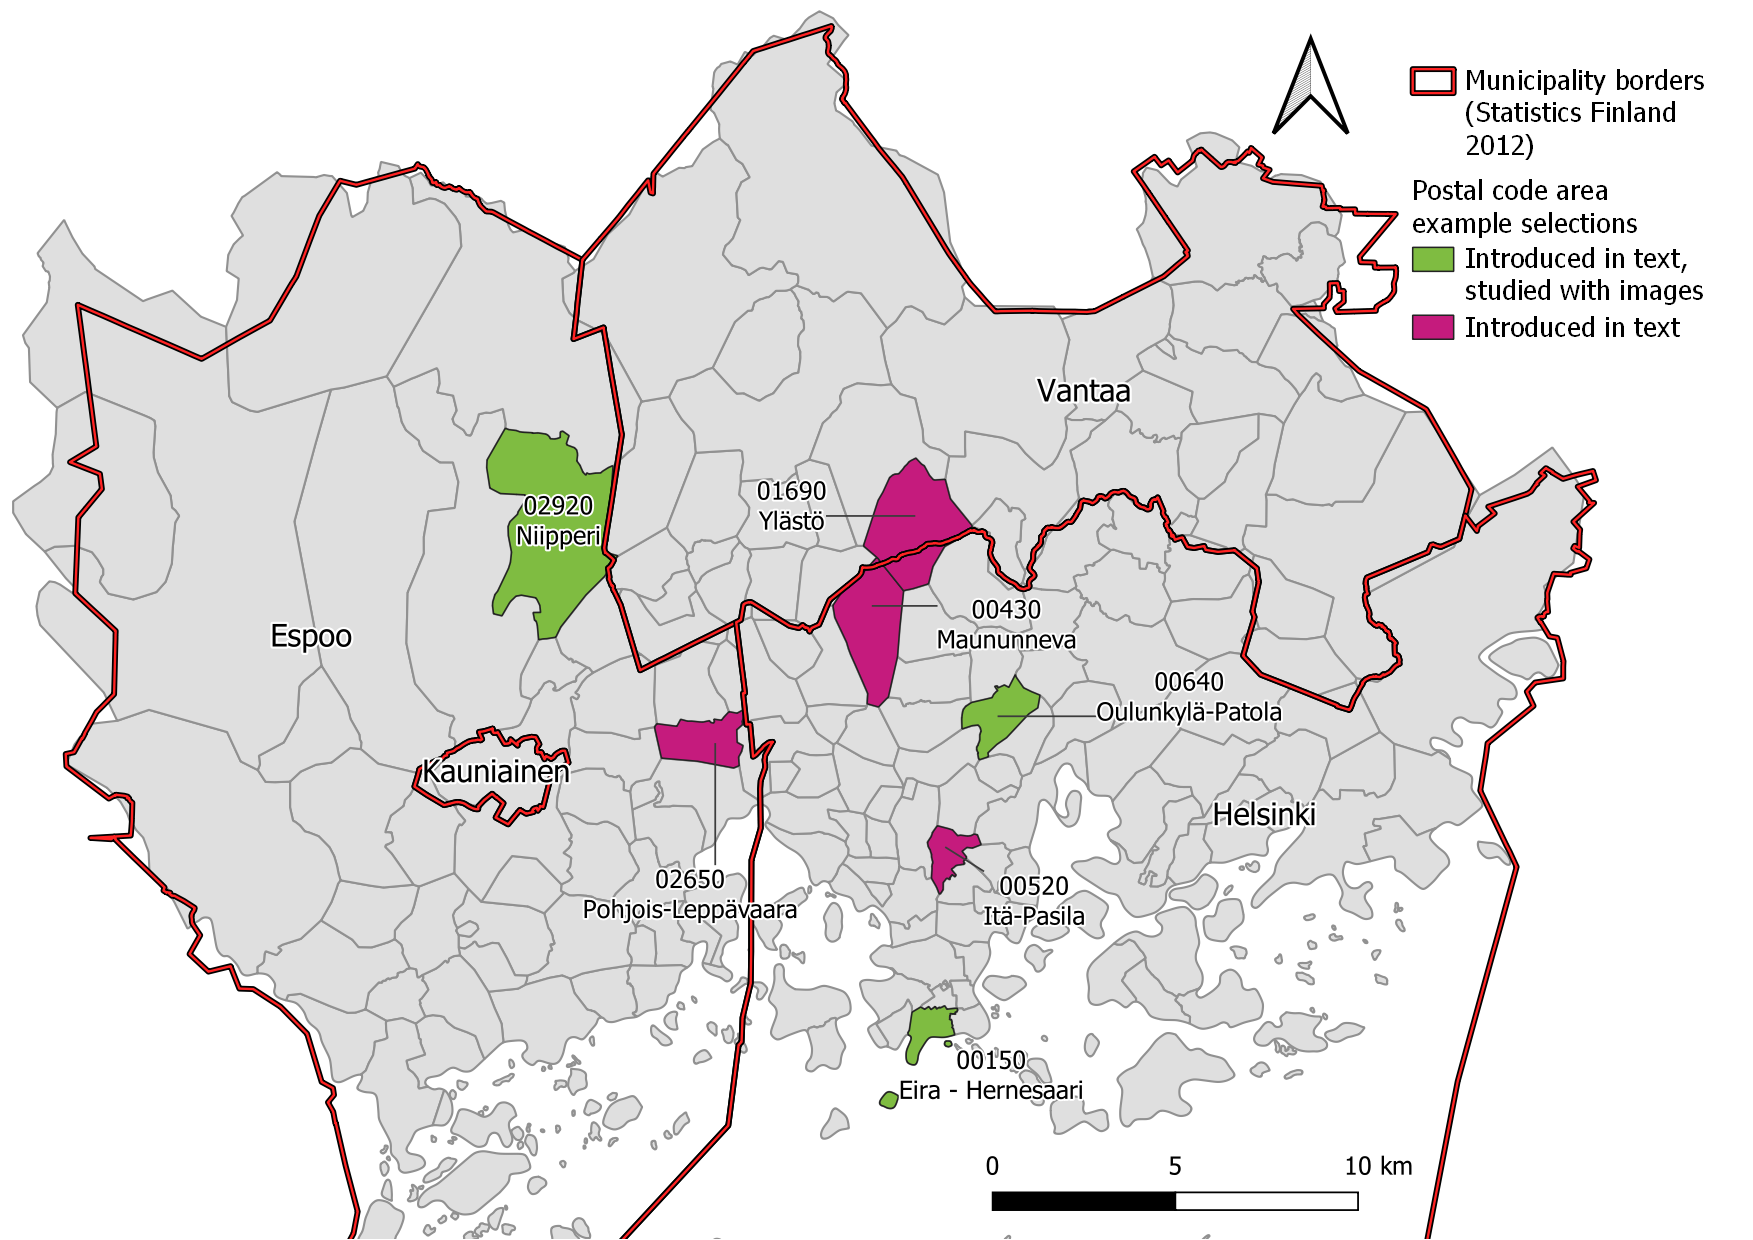
\includegraphics[trim={0 0.2cm 0 0},clip,width=\textwidth]{images/results_comparison_examplezips.png}
    \caption[Postal code areas selected for in-depth results review]{Postal code areas selected for in-depth results review.}%
    \label{fig:ykrzone_selections_map}%
\end{figure}

The selected postal code areas represent functionally different parts of the research area. 00150 Eira-Hernesaari (Center walking zone) is located at the southern tip of Helsinginniemi where all possible travel options for private car are time intensive. 00520 Itä-Pasila (Center periphery zone) is in the immediate vicinity of the center of Helsinki, is densely built, and is equipped with better travel options for the private car than Eira-Hernesaari. 02650 Pohjois-Leppävaara (Subcenter walking zone) represents an important subcenter in the research area with large amounts of office space, a major shopping mall, and a large population. It is a major residential area in Espoo, and it has a good access to major roads. 00640 Oulunkylä-Patola (Intensive transit zone) is also mostly a residential area with extensive public transport connections as well as access to major road infrastructure of Helsinki Capital Region, namely the Ring I beltway and the Finnish national road 3 to Tampere. 00430 Maununneva (Transit zone) is a residential area situated just next to the Finnish national highway 3, but with limited motorway interchanges. Its eastern side hugs the Central Park of Helsinki and is littered with small neighborhood roads. 02920 Niipperi (Automobile zone) is characterised as an area of detached housing where public transport coverage is scarce. 01690 Ylästö (novalue) was selected to represent postal code areas which were outside of the YKR zones classification according to the thesis calculation method. These areas can be centers of local activity, but lack a combination of population, commercial interaction and public transport connections to belong in any of the proper \code{ykr\_zone} groups (\textcolor{red}{cite ykrvyöhykkeet}). It is then indicative to use these areas as representatives of the whole research area, as the breadth of the data available in the travel time comparison application is much too plentiful to be presented in full in tables or individual images. The results will delve further into the proportion of the parking process in the cases of 00150 Eira-Hernesaari, 00640 Oulunkylä-Patola, and 02920 Niipperi.

Table~\ref{tab:comparison_parkingprocess_signif} presents the driving segments and parking process segments of several different example travel chains. In these examples, the parking process is a significant part of the travel chains. In most cases the parking process share diminishes the longer the travel chain is in duration and kilometers, but driving to the center of Helsinki is an exception of this because of the long mean \code{parktime} and \code{walktime} values. When comparing the parking process length between thesis survey and the durations used in \textit{TTM}, thesis parking process can be up to six times longer than that of in \textit{TTM}.

\begin{hyphenrules}{nohyphenation}
    \begin{table}[H]
        \centering
        \caption[Parking process significance]{Proportion of the parking process in example travel chains utilising thesis survey data. Mean parking process duration is static data and does not change for individual destination postal code areas.}
        \label{tab:comparison_parkingprocess_signif}
        \scalebox{0.75}
        {\begin{tabular}{>{\raggedleft\arraybackslash}p{4cm} lccCccCccc}
            \toprule
        	& & \multicolumn{3}{>{\centering}p{3cm}}{Mean driving time duration, \textit{TTM} data (min)} & \multicolumn{3}{>{\centering}p{3cm}}{Mean parking process duration, survey data (min)} & \multicolumn{3}{>{\centering}p{3cm}}{Parking process share of the total travel chain (\%)} \\
        	\cmidrule(lr{\tbspace}){3-5} \cmidrule(lr{\tbspace}){6-8} \cmidrule(lr){9-11}
        	Origin & Destination &          rush & mid & all &          rush & mid & all &      rush & mid & all \\
            \midrule
            \multirow{7}{4cm}{00150 Eira - Hernesaari (Center walking zone)} & 00150 & 5.12 & 4.68 & 4.48 & 11.25 & 17.40 & 14.16 & 2.20* & 3.72* & 3.16*
 \\
            & 00520 &                       24.21 & 20.25 & 18.53 &     13.59 & 11.67 & 13.58 & 0.56 & 0.58 & 0.73 \\
            & 02650 &                       33.50 & 29.16 & 26.20 &     4.11 & 7.47 & 7.08 &    0.12 & 0.26 & 0.27 \\
            & 00640 &                       34.18 & 29.11 & 26.48 &     5.00 & 7.33 & 6.09 &    0.15 & 0.25 & 0.23 \\
            & 00430 &                       37.53 & 32.49 & 29.27 &     6.34 & 8.33 & 4.47 &    0.17 & 0.26 & 0.15 \\
            & 02920 &                       52.02 & 43.61 & 40.94 &     4.00 & 6.00 & 4.33 &    0.08 & 0.14 & 0.11 \\
            & 01690 &                       48.06 & 41.74 & 37.90 &     0.00 & 7.00 & 3.75 &    0.00 & 0.17 & 0.10 \\
            \arrayrulecolor{black}\midrule
            
            \multirow{7}{4cm}{00520 Itä-Pasila (Center periphery zone)} & 00150 & 22.89 & 18.87 & 17.38 & 11.25 & 17.40 & 14.16 & 0.49 & 0.92 & 0.81 \\
            & 00520 &                       6.77 & 5.47 & 5.11 &        13.59 & 11.67 & 13.58 & 2.01* & 2.13* & 2.66* \\
            & 02650 &                       25.85 & 21.90 & 19.76 &     4.11 & 7.47 & 7.08 &    0.16 & 0.34 & 0.36 \\
            & 00640 &                       16.00 & 13.06 & 12.20 &     5.00 & 7.33 & 6.09 &    0.31 & 0.56 & 0.50 \\
            & 00430 &                       23.73 & 19.76 & 18.25 &     6.34 & 8.33 & 4.47 &    0.27 & 0.42 & 0.24 \\
            & 02920 &                       41.87 & 34.71 & 32.36 &     4.00 & 6.00 & 4.33 &    0.10 & 0.17 & 0.13 \\
            & 01690 &                       31.06 & 26.57 & 24.61 &     0.00 & 7.00 & 3.75 &    0.00 & 0.26 & 0.15 \\
            \arrayrulecolor{black}\midrule
            
            \multirow{7}{4cm}{02650 Pohjois-Leppävaara (Subcenter walking zone)} & 00150 & 34.28 & 29.42 & 26.46 & 11.25 & 17.40 & 14.16 & 0.33 & 0.59 & 0.54 \\
            & 00520 &                       26.62 & 22.10 & 20.23 &     13.59 & 11.67 & 13.58 & 0.51 & 0.53 & 0.67 \\
            & 02650 &                       5.53 & 4.92 & 4.53 &        4.11 & 7.47 & 7.08 &    0.74 & 1.52* & 1.56* \\
            & 00640 &                       20.82 & 18.52 & 16.70 &     5.00 & 7.33 & 6.09 &    0.24 & 0.40 & 0.36 \\
            & 00430 &                       19.06 & 17.30 & 15.52 &     6.34 & 8.33 & 4.47 &    0.33 & 0.48 & 0.29 \\
            & 02920 &                       27.51 & 23.78 & 22.19 &     4.00 & 6.00 & 4.33 &    0.15 & 0.25 & 0.20 \\
            & 01690 &                       29.80 & 26.52 & 24.15 &     0.00 & 7.00 & 3.75 &    0.00 & 0.26 & 0.16 \\
            \arrayrulecolor{black}\midrule
            
            \multirow{7}{4cm}{00640 Oulunkylä-Patola (Intensive transit zone)} & 00150 & 35.33 & 29.62 & 27.06 & 11.25 & 17.40 & 14.16 & 0.32 & 0.59 & 0.52 \\
            & 00520 &                       17.20 & 14.24 & 13.11 &     13.59 & 11.67 & 13.58 & 0.79 & 0.82 & 1.04* \\
            & 02650 &                       20.83 & 18.17 & 16.50 &     4.11 & 7.47 & 7.08 &    0.20 & 0.41 & 0.43 \\
            & 00640 &                       4.44 & 3.87 & 3.71 &        5.00 & 7.33 & 6.09 &    1.13* & 1.89* & 1.64* \\
            & 00430 &                       17.04 & 14.54 & 13.59 &     6.34 & 8.33 & 4.47 &    0.37 & 0.57 & 0.33 \\
            & 02920 &                       35.87 & 30.31 & 28.39 &     4.00 & 6.00 & 4.33 &    0.11 & 0.20 & 0.15 \\
            & 01690 &                       23.76 & 20.42 & 19.24 &     0.00 & 7.00 & 3.75 &    0.00 & 0.34 & 0.19 \\
            \arrayrulecolor{black}\midrule
            
            \multirow{7}{4cm}{00430 Maununneva (Transit zone)} & 00150 & 38.60 & 32.89 & 29.82 & 11.25 & 17.40 & 14.16 & 0.29 & 0.53 & 0.47 \\
            & 00520 &                       24.58 & 21.01 & 19.05 &     13.59 & 11.67 & 13.58 & 0.55 & 0.56 & 0.71 \\
            & 02650 &                       17.32 & 15.60 & 14.07 &     4.11 & 7.47 & 7.08 &    0.24 & 0.48 & 0.50 \\
            & 00640 &                       17.13 & 14.94 & 13.91 &     5.00 & 7.33 & 6.09 &    0.29 & 0.49 & 0.44 \\
            & 00430 &                       8.72 & 7.71 & 7.28 &        6.34 & 8.33 & 4.47 &    0.73 & 1.08* & 0.61 \\
            & 02920 &                       29.62 & 25.98 & 23.87 &     4.00 & 6.00 & 4.33 &    0.14 & 0.23 & 0.18 \\
            & 01690 &                       17.51 & 15.74 & 14.77 &     0.00 & 7.00 & 3.75 &    0.00 & 0.44 & 0.25 \\
            \arrayrulecolor{black}\midrule
            
            \multirow{7}{4cm}{02920 Niipperi (Automobile zone)} & 00150 & 54.19 & 44.85 & 41.98 & 11.25 & 17.40 & 14.16 & 0.21 & 0.39 & 0.34 \\
            & 00520 &                       42.85 & 35.41 & 33.00 &     13.59 & 11.67 & 13.58 & 0.32 & 0.33 & 0.41 \\
            & 02650 &                       26.80 & 23.17 & 21.61 &     4.11 & 7.47 & 7.08 &    0.15 & 0.32 & 0.33 \\
            & 00640 &                       36.58 & 30.88 & 28.90 &     5.00 & 7.33 & 6.09 &    0.14 & 0.24 & 0.21 \\
            & 00430 &                       29.15 & 25.82 & 23.73 &     6.34 & 8.33 & 4.47 &    0.22 & 0.32 & 0.19 \\
            & 02920 &                       9.75 & 8.97 & 8.49 &        4.00 & 6.00 & 4.33 &    0.41 & 0.67 & 0.51 \\
            & 01690 &                       29.31 & 25.95 & 24.08 &     0.00 & 7.00 & 3.75 &    0.00 & 0.27 & 0.16 \\
            \arrayrulecolor{black}\midrule
            
            \multirow{7}{4cm}{01690 Ylästö (novalue)} & 00150 & 48.65 & 41.47 & 37.90 & 11.25 & 17.40 & 14.16 & 0.23 & 0.42 & 0.37 \\
            & 00520 &                       32.15 & 27.31 & 25.21 &     13.59 & 11.67 & 13.58 & 0.42 & 0.43 & 0.54 \\
            & 02650 &                       27.73 & 24.48 & 22.38 &     4.11 & 7.47 & 7.08 &    0.15 & 0.31 & 0.32 \\
            & 00640 &                       23.95 & 20.28 & 19.23 &     5.00 & 7.33 & 6.09 &    0.21 & 0.36 & 0.32 \\
            & 00430 &                       18.39 & 16.31 & 15.36 &     6.34 & 8.33 & 4.47 &    0.34 & 0.51 & 0.29 \\
            & 02920 &                       29.88 & 26.41 & 24.35 &     4.00 & 6.00 & 4.33 &    0.13 & 0.23 & 0.18 \\
            & 01690 &                       8.45 & 7.87 & 7.56 &        0.00 & 7.00 & 3.75 &    0.00 & 0.89 & 0.50 \\
            \bottomrule
            
            % A multicolumn pretending to be a footnote, works well for this cause
            \multicolumn{11}{ p{18cm} }{\textsuperscript{*}\footnotesize{Thesis research survey data parking process is longer than the entire driving time segment calculated from Helsinki Region Travel Time Matrix 2018.}}
        \end{tabular}}
    \end{table}
\end{hyphenrules}

The proportion of the parking process from the starting postal code area of 00150 Eira-Hernesaari appears relatively even when viewing the survey data with equal intervals. The southern part of Helsinginniemi accumulates the largest parking process shares. In the \code{pct} data, additionally, it is quite commonplace to end up in a situation where the calculated parking process duration is longer than the calculated \textit{TTM} mean driving time to a destination postal code area.

During rush hour traffic, the proportion of the parking process in travel chains starting from 00150 Eira-Hernesaari is highest in the center of Helsinki (figure~\ref{fig:compare_msc_r_pct_00150}). Outside the center, 00670 Paloheinä, Helsinki (parking process 39 \% of the total travel chain duration), 00870 Etelä-Laajasalo, Helsinki (43 \%), and 01400 Rekola, Vantaa (66 \%) stand out with lengthy parking processes compared to \code{drivetime}. In addition to the occasionally alarmingly long parking processes, some postal code areas report parking process proportions of zero percent, according to the survey data. Some of these are, for example, 00830 Tammisalo in Helsinki, 02940 Lippajärvi-Järvenperä in Espoo, and 01690 Ylästö in Vantaa.

During midday traffic, the general outline of the parking process durations starting from 00150 Eira-Hernesaari stays similar compared to rush hour traffic (figure~\ref{fig:compare_msc_m_pct_00150}). Some particularly long parking processes may be found from 01750 Keimola, Vantaa (parking process 95 \% of the total travel chain duration, an anomalous survey result), 00590 Kaitalahti, Helsinki (42 \%), and 02100 Tapiola, Espoo (43 \%). A midday parking process share of 0 \% is only present in 02820 Nupuri-Nuuksio, Espoo.

Using all available survey data and the full \textit{TTM} data, all postal code areas can be represented (figure~\ref{fig:compare_msc_all_pct_00150}). This data largely follows the trend of rush hour and midday data of the origin postal code area 00150 Eira-Hernesaari. Utilising this aggregated variable, long parking processes are found from 02100 Tapiola in Espoo (55 \%), Kulosaari in Helsinki (58 \%), and 00590 Kaitalahti in Helsinki (44 \%). The parking process proportions of subcenters of the Helsinki Capital Region slightly stand out from the data, but this is an inconclusive observation as sparsely populated locations such as 01750 Keimola may also receive large parking process shares.

% trim={<left> <lower> <right> <upper>}
\begin{figure}[H]%
    \centering
    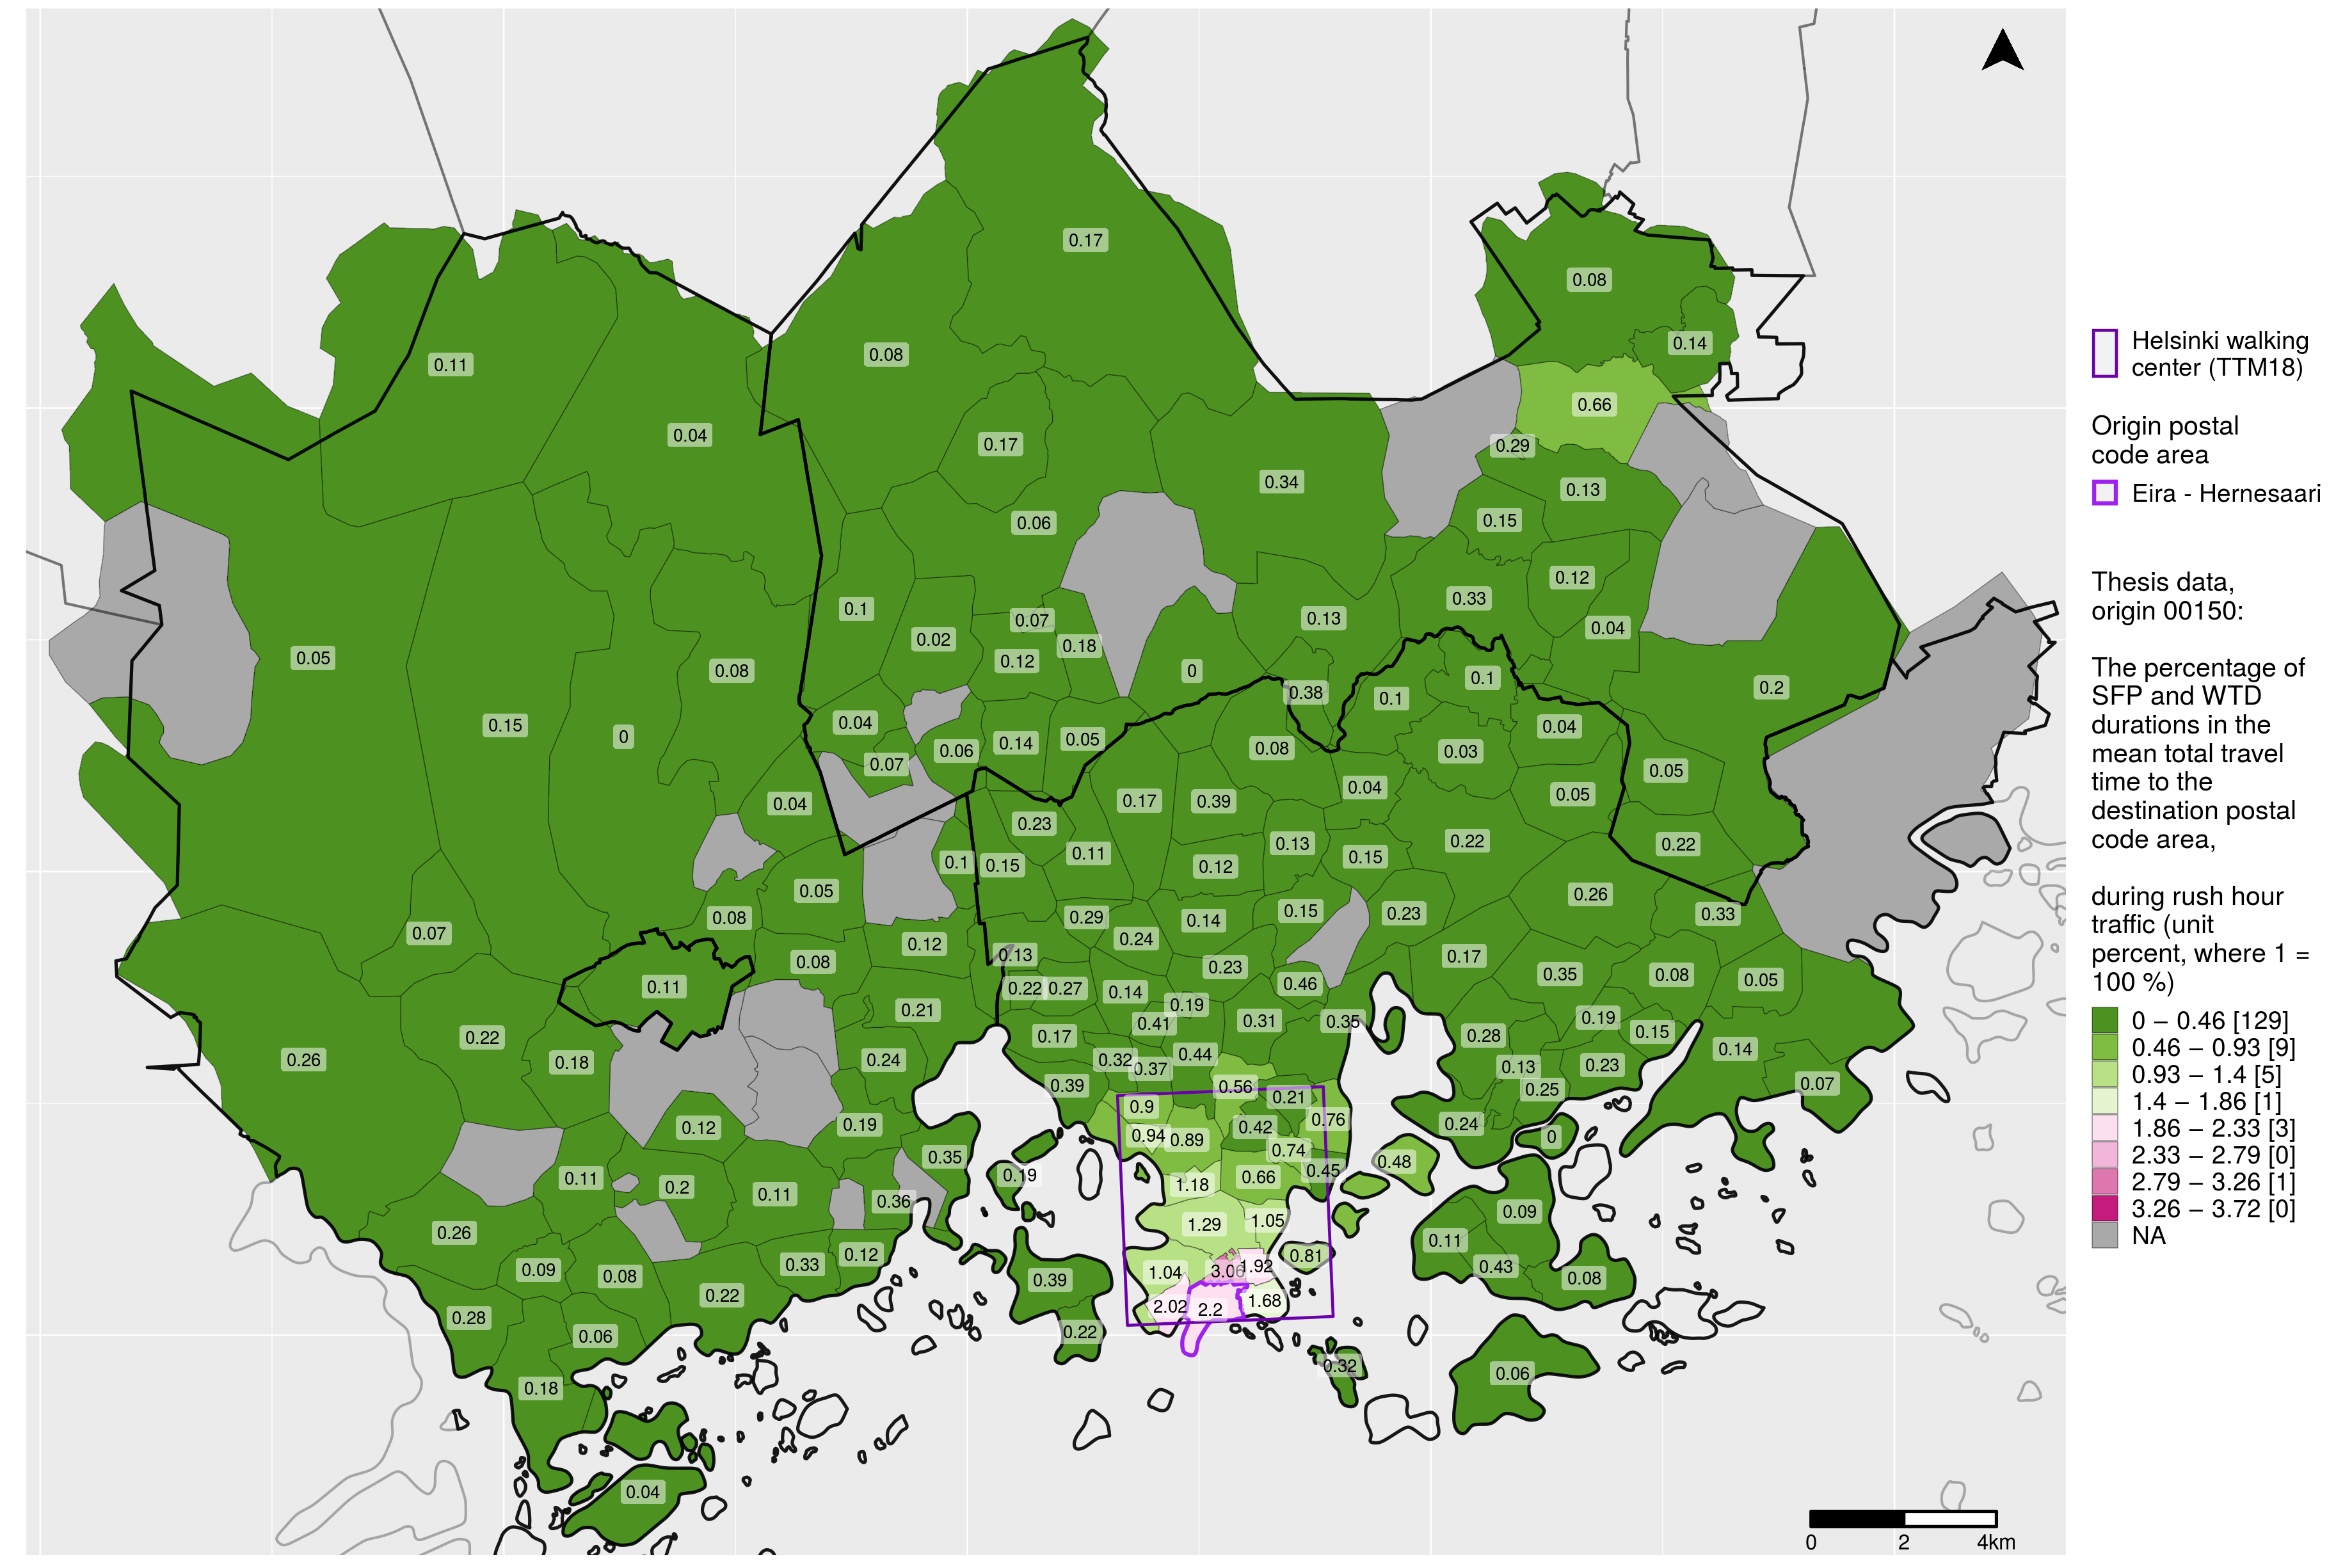
\includegraphics[trim={0.9cm 0.3cm 0.25cm 0.3cm},clip,width=\textwidth]{images/compare_traveltimes_mapfill-msc_r_pct_fromzip-00150_28-09-2020.png}
    \caption[Parking process proportion from Eira-Hernesaari, rush hour traffic]{The parking process proportion in the total travel chain, in rush hour traffic, starting from 00150 Eira-Hernesaari.}%
    \label{fig:compare_msc_r_pct_00150}%
\end{figure}

\begin{figure}[H]%
    \centering
    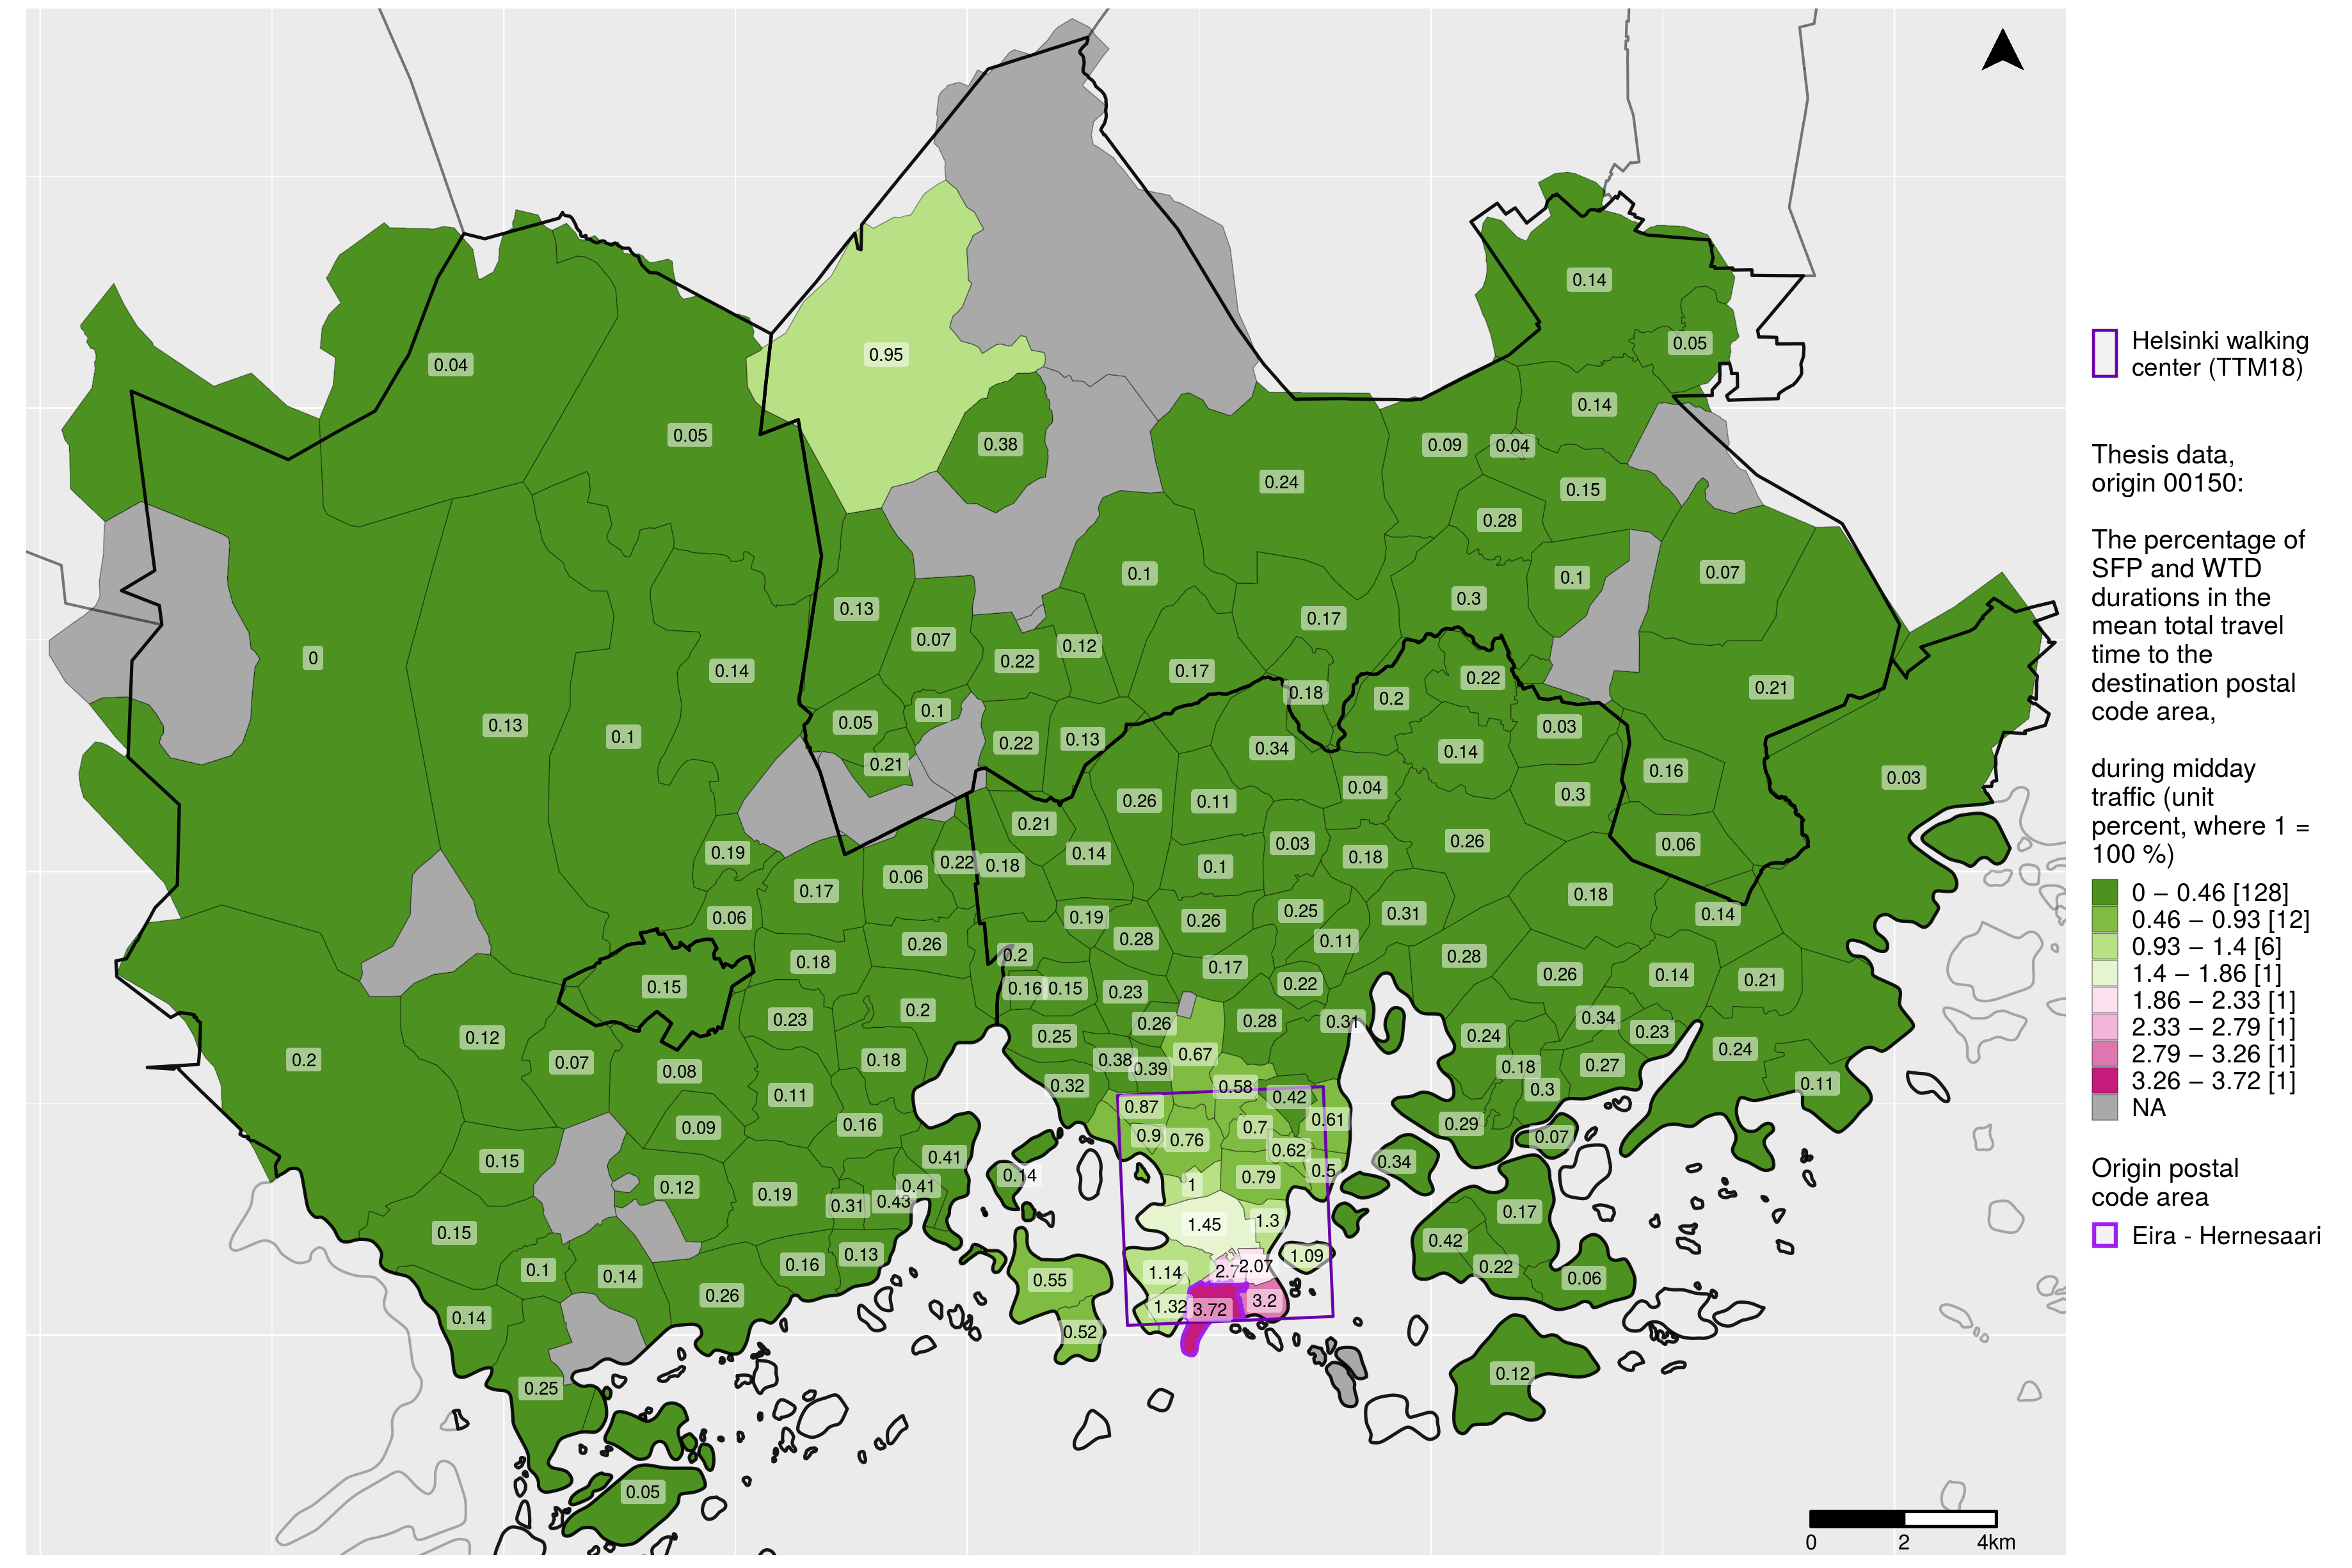
\includegraphics[trim={0.9cm 0.3cm 0.25cm 0.3cm},clip,width=\textwidth]{images/compare_traveltimes_mapfill-msc_m_pct_fromzip-00150_28-09-2020.png}
    \caption[Parking process proportion from Eira-Hernesaari, midday traffic]{The parking process proportion in the total travel chain, in midday traffic, starting from 00150 Eira-Hernesaari.}%
    \label{fig:compare_msc_m_pct_00150}%
\end{figure}

\begin{figure}[H]%
    \centering
    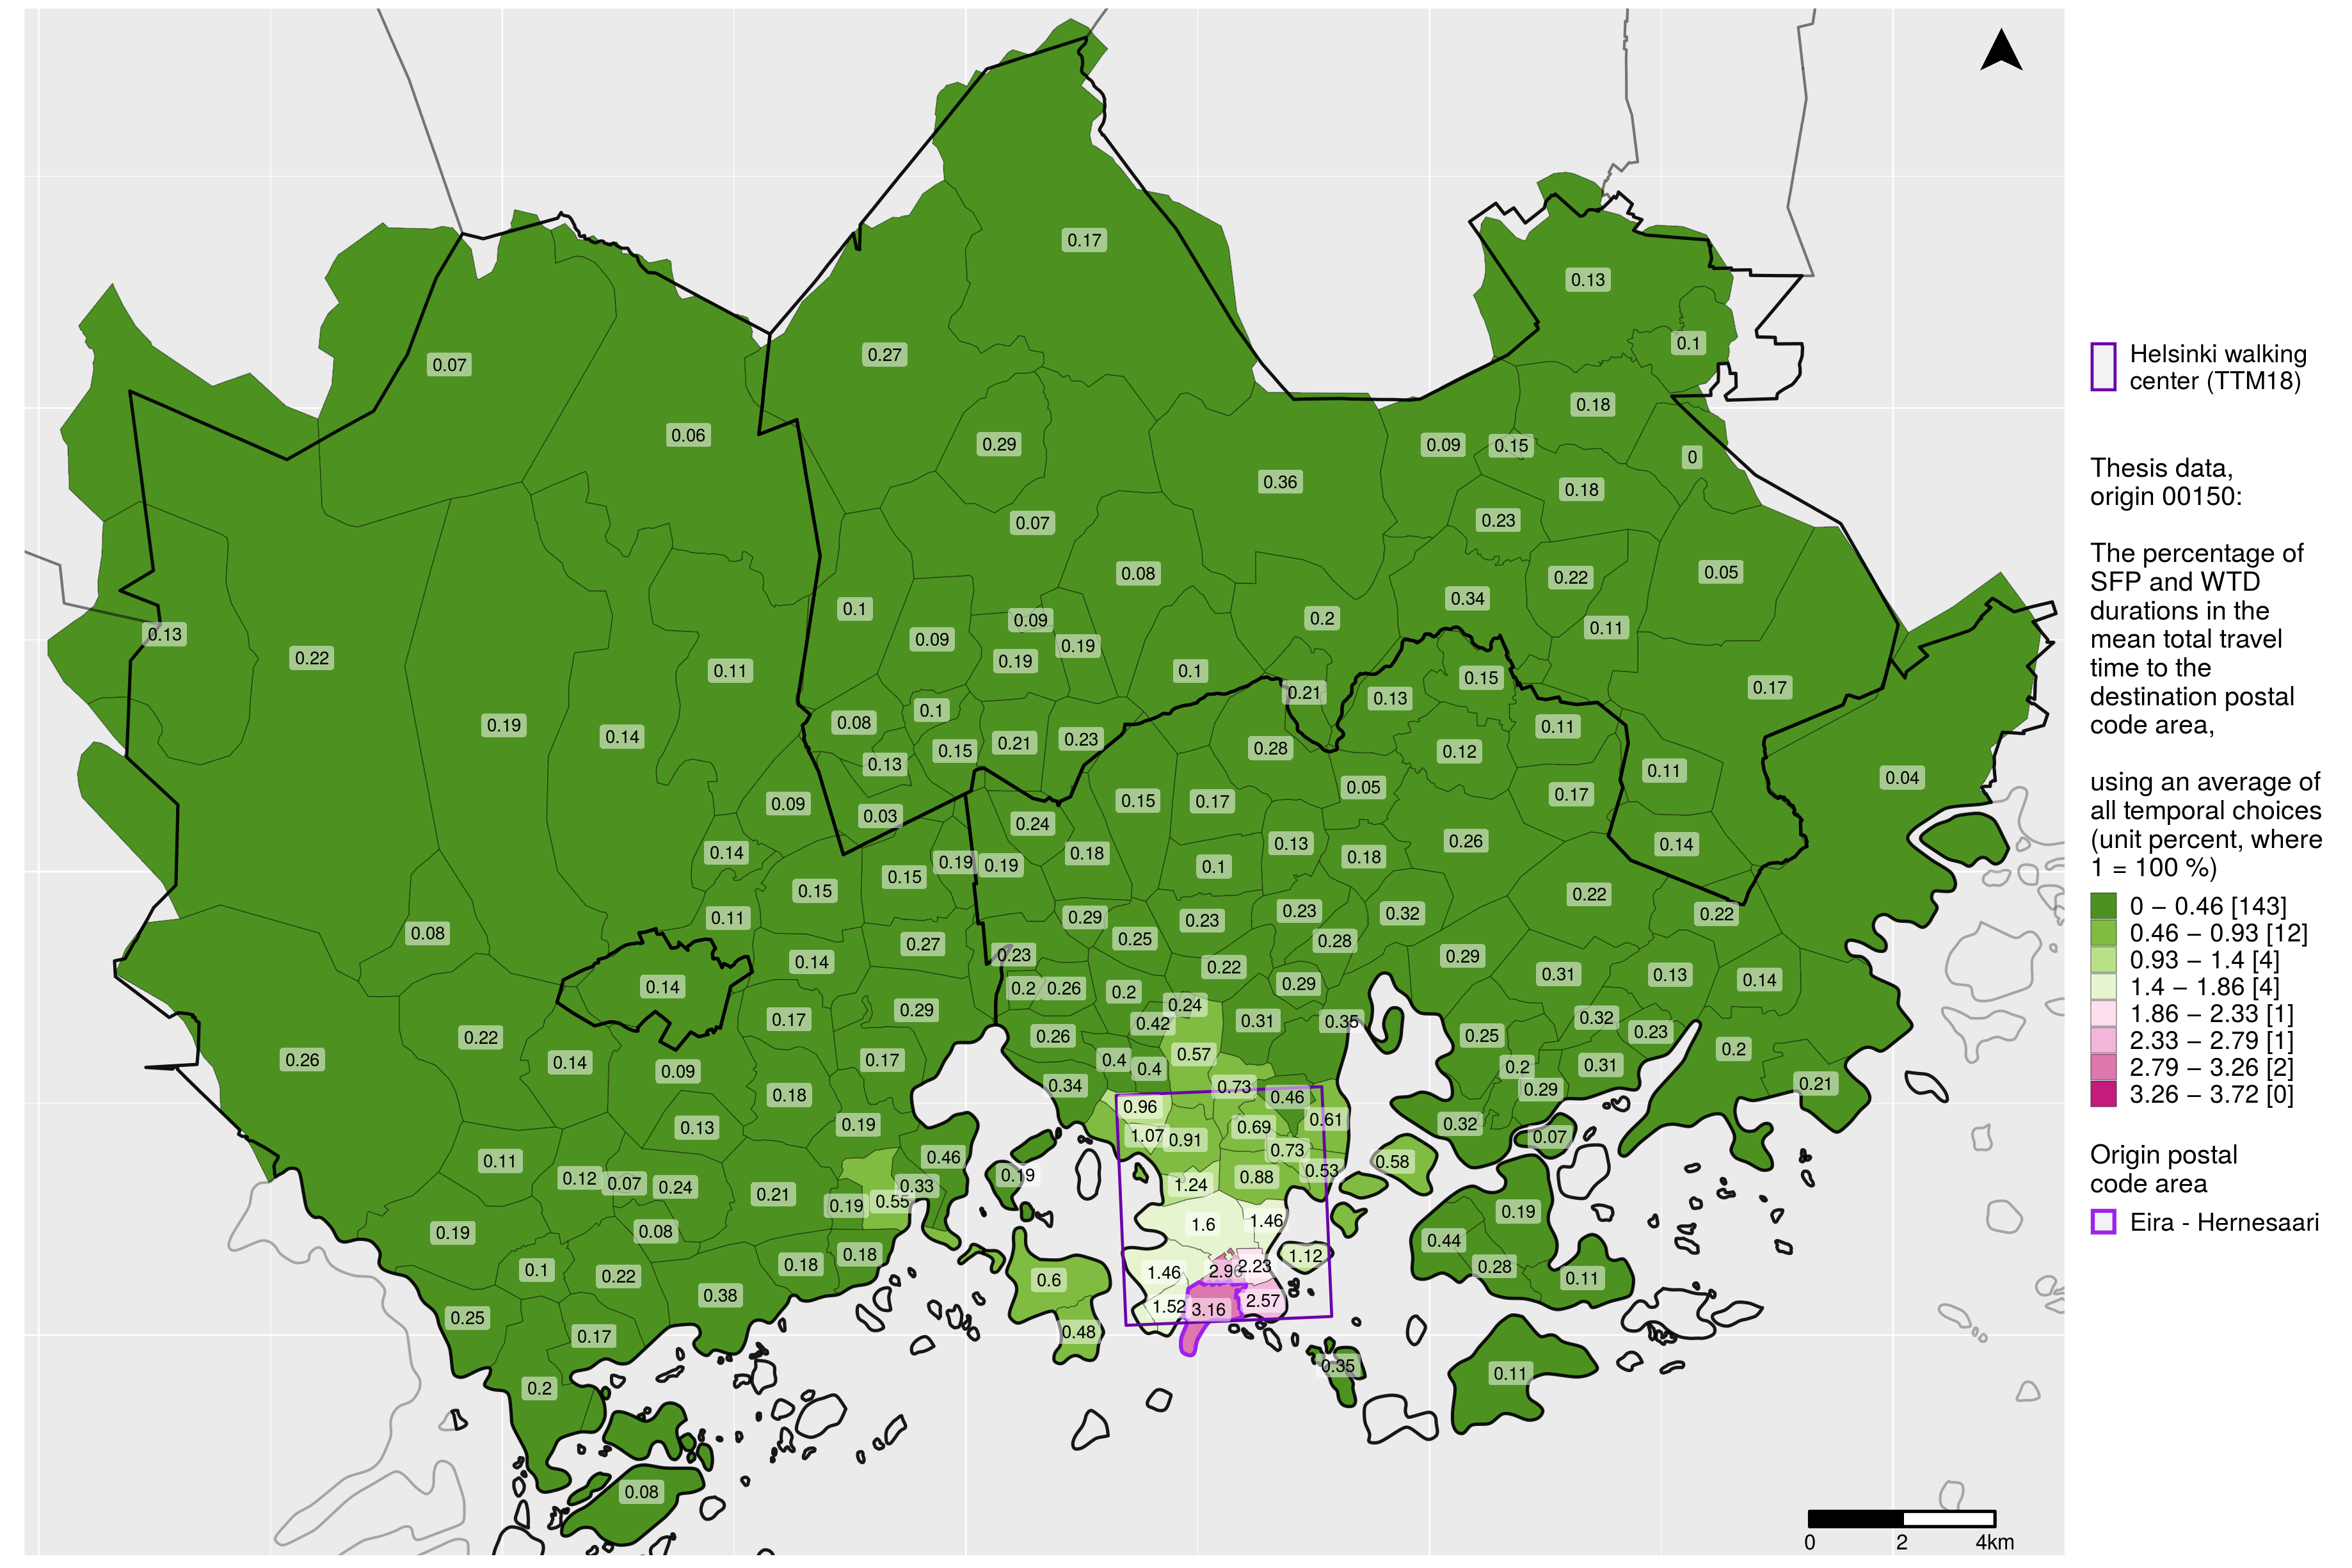
\includegraphics[trim={0.9cm 0.3cm 0.25cm 0.3cm},clip,width=\textwidth]{images/compare_traveltimes_mapfill-msc_all_pct_fromzip-00150_28-09-2020.png}
    \caption[Parking process proportion from Eira-Hernesaari, all temporal values]{The parking process proportion in the total travel chain, using all available temporal values, starting from 00150 Eira-Hernesaari.}%
    \label{fig:compare_msc_all_pct_00150}%
\end{figure}

The proportion of the parking process fluctuates spatially when viewing the percentual data with 00640 Oulunkylä-Patola as the origin postal code area. For rush hour traffic, the largest shares of the total travel chains can be found in the general vicinity of the origin postal code area, with prongs extending to the center of Helsinki and to eastern Helsinki (figure~\ref{fig:compare_msc_r_pct_00640}). Excluding the destination postal code areas where the parking process is longer than the calculated \code{drivetime}, long parking process shares may be located at 00270 Pohjois-Meilahti in Helsinki (87 \% of the total travel chain duration), 00920 Myllypuro in Helsinki (72 \%), and 01530 Veromiehenkylä in Vantaa (68 \%). It is notable that 00640 Oulunkylä-Patola has generally more valid percentual values (parking process share is less than the total driving segment of the travel chain) than 00150 Eira-Hernesaari as fewer postal code areas have their parking process durations exceed that of their \code{drivetime} values.

In midday traffic, the proportion of the parking process in travel chains from the origin 00640 Oulunkylä-Patola shows long parking process shares for the most parts of Helsinki and for a branch reaching northeast to Vantaa (figure~\ref{fig:compare_msc_m_pct_00640}). For midday traffic, long parking process shares are calculated for 01300 Tikkurila in Vantaa (68 \%), and 00510 Etu-Vallila--Alppila in Helsinki (83 \%). In most of Espoo parking process shares are less than 30 percent, with the longest found from 02650 Pohjois-Leppävaara in Espoo (41 \%).

If all available temporal data is employed in thesis survey data and \textit{TTM}, extreme values recorded in \code{parktime} and \code{walktime} are honed away and a rough circular shape of long parking process shares may be observed around 00640 Oulunkylä-Patola (figure~\ref{fig:compare_msc_all_pct_00640}). Using this variable the majority of the center of Helsinki receives parking process shares of more than 60 percent. In general, most of the largest parking process shares are located inside the Ring I beltway with the exception of Vantaa's 01300 Tikkurila (76 \%) and 01530 Veromiehenkylä (71 \%).

\begin{figure}[H]%
    \centering
    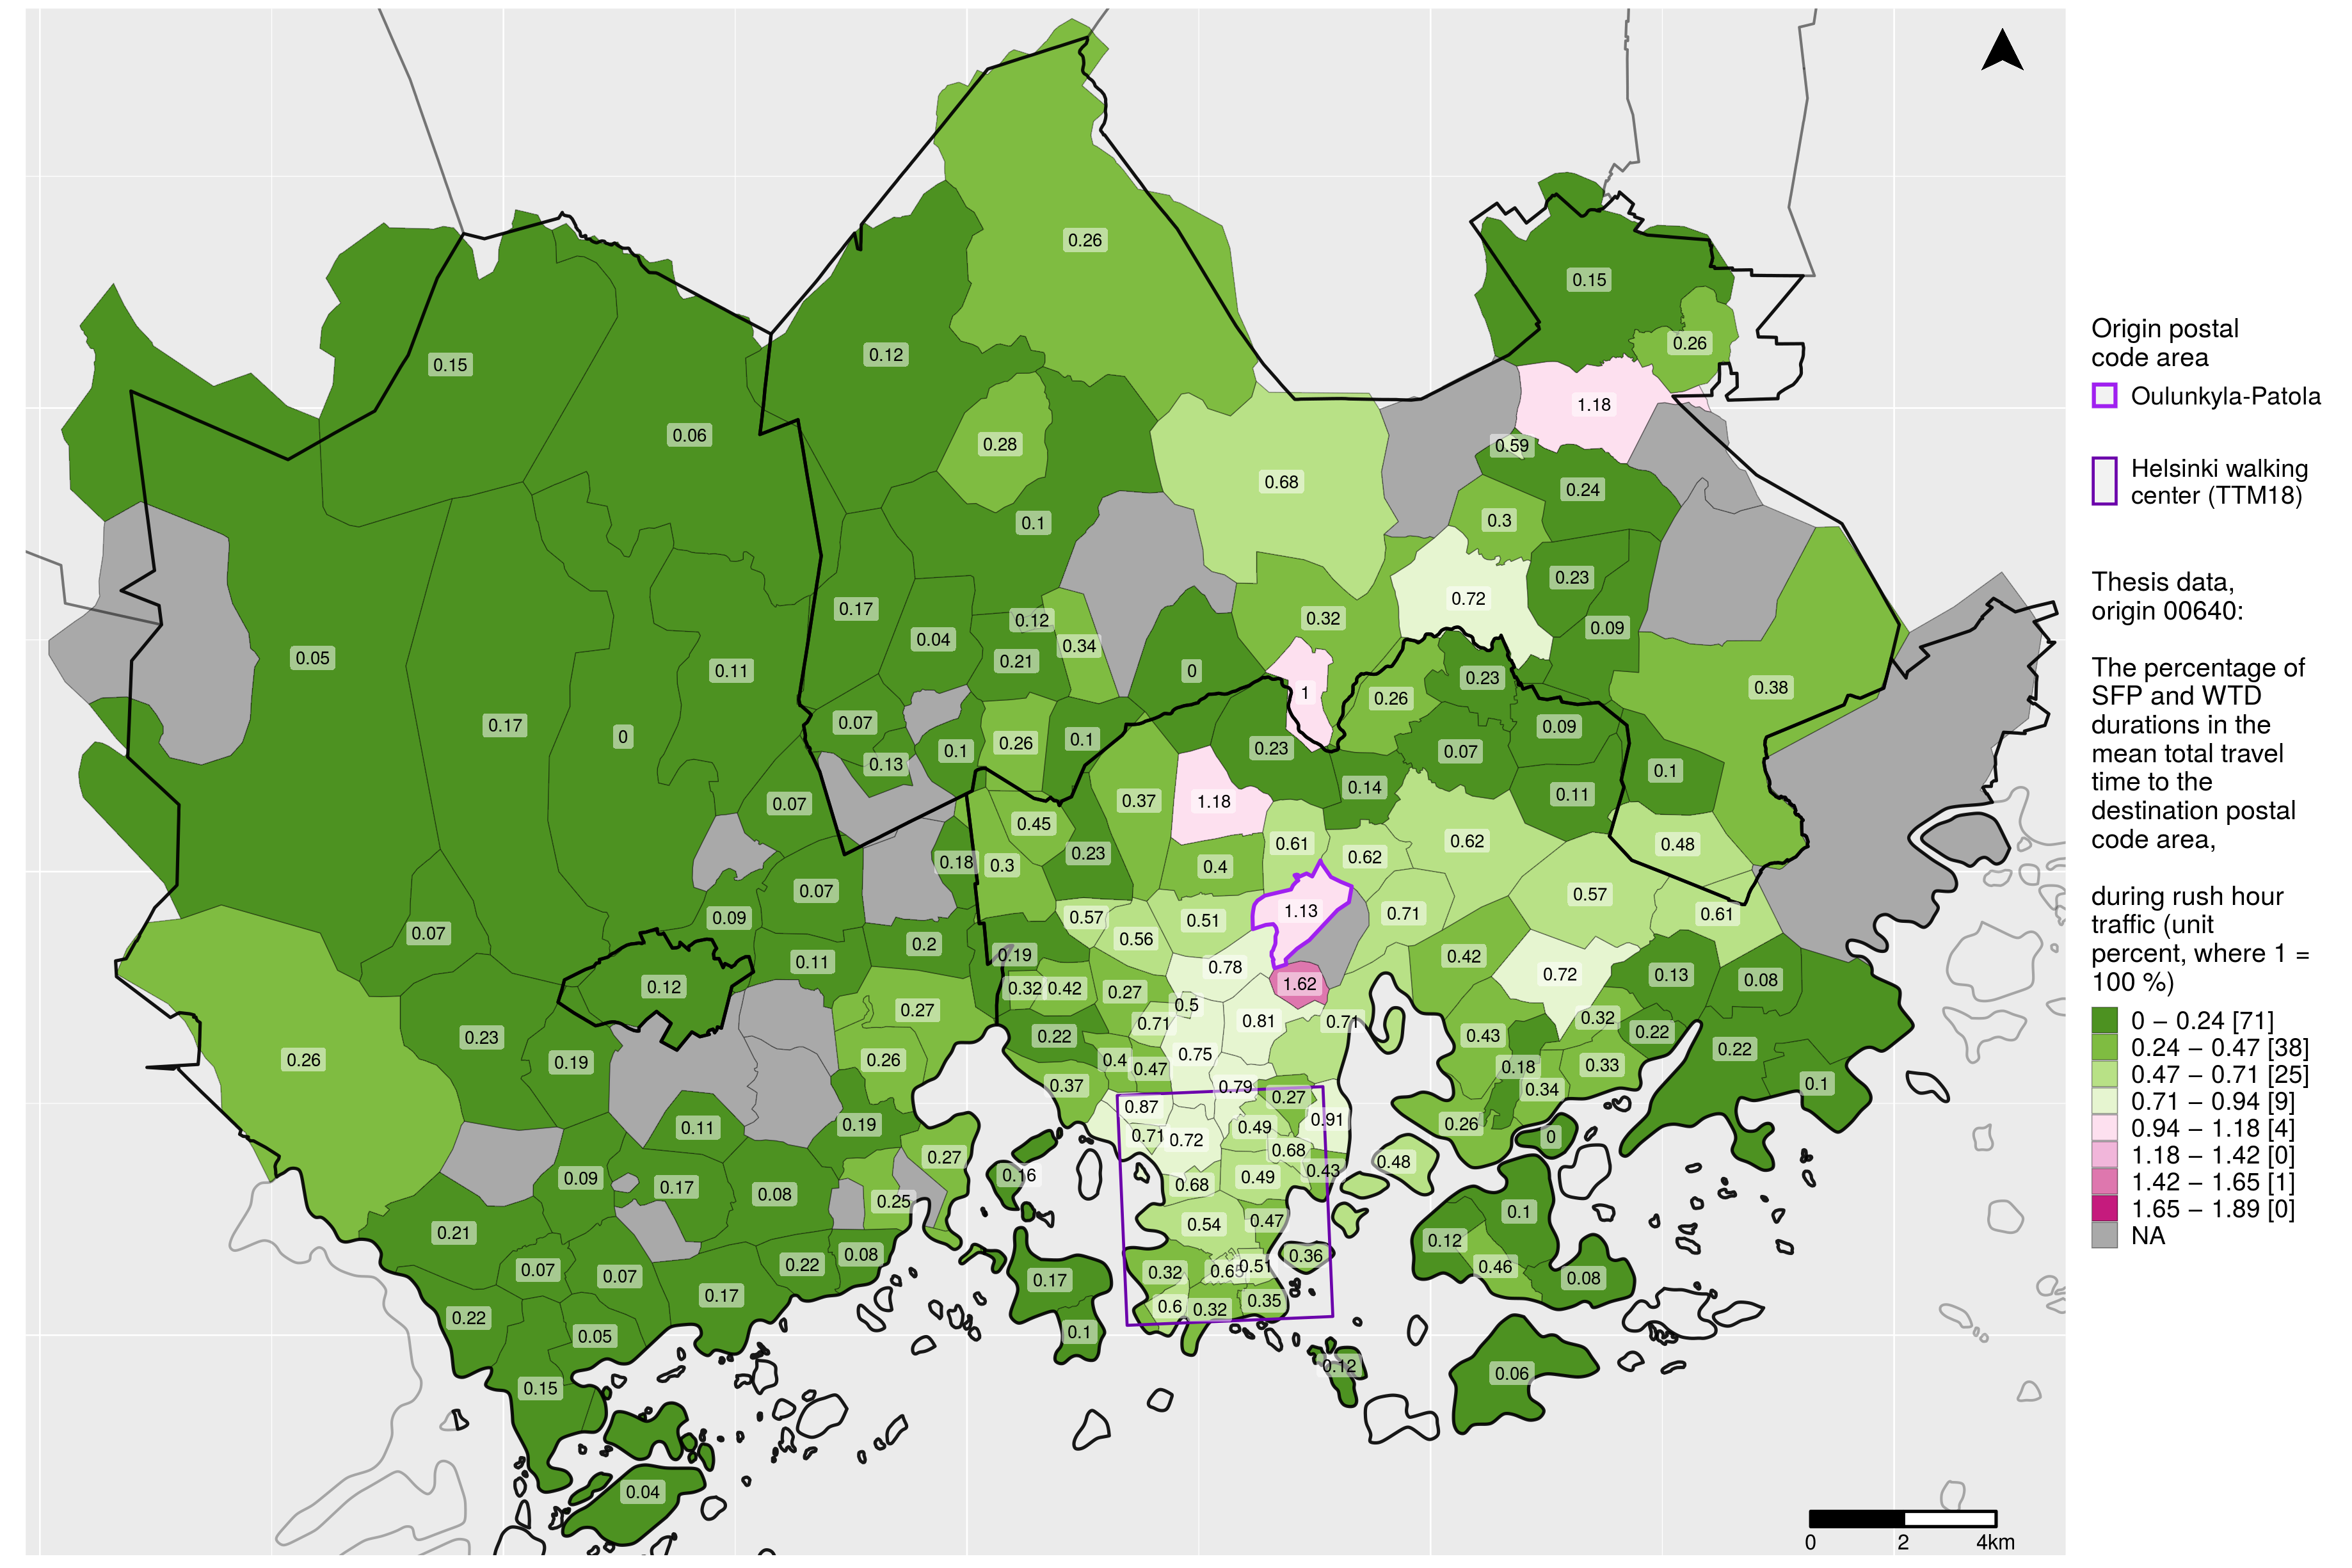
\includegraphics[trim={0.9cm 0.3cm 0.25cm 0.3cm},clip,width=\textwidth]{images/compare_traveltimes_mapfill-msc_r_pct_fromzip-00640_28-09-2020.png}
    \caption[Parking process proportion from Oulunkylä-Patola, rush hour traffic]{The parking process proportion in the total travel chain, in rush hour traffic, starting from 00640 Oulunkylä-Patola.}%
    \label{fig:compare_msc_r_pct_00640}%
\end{figure}

\begin{figure}[H]%
    \centering
    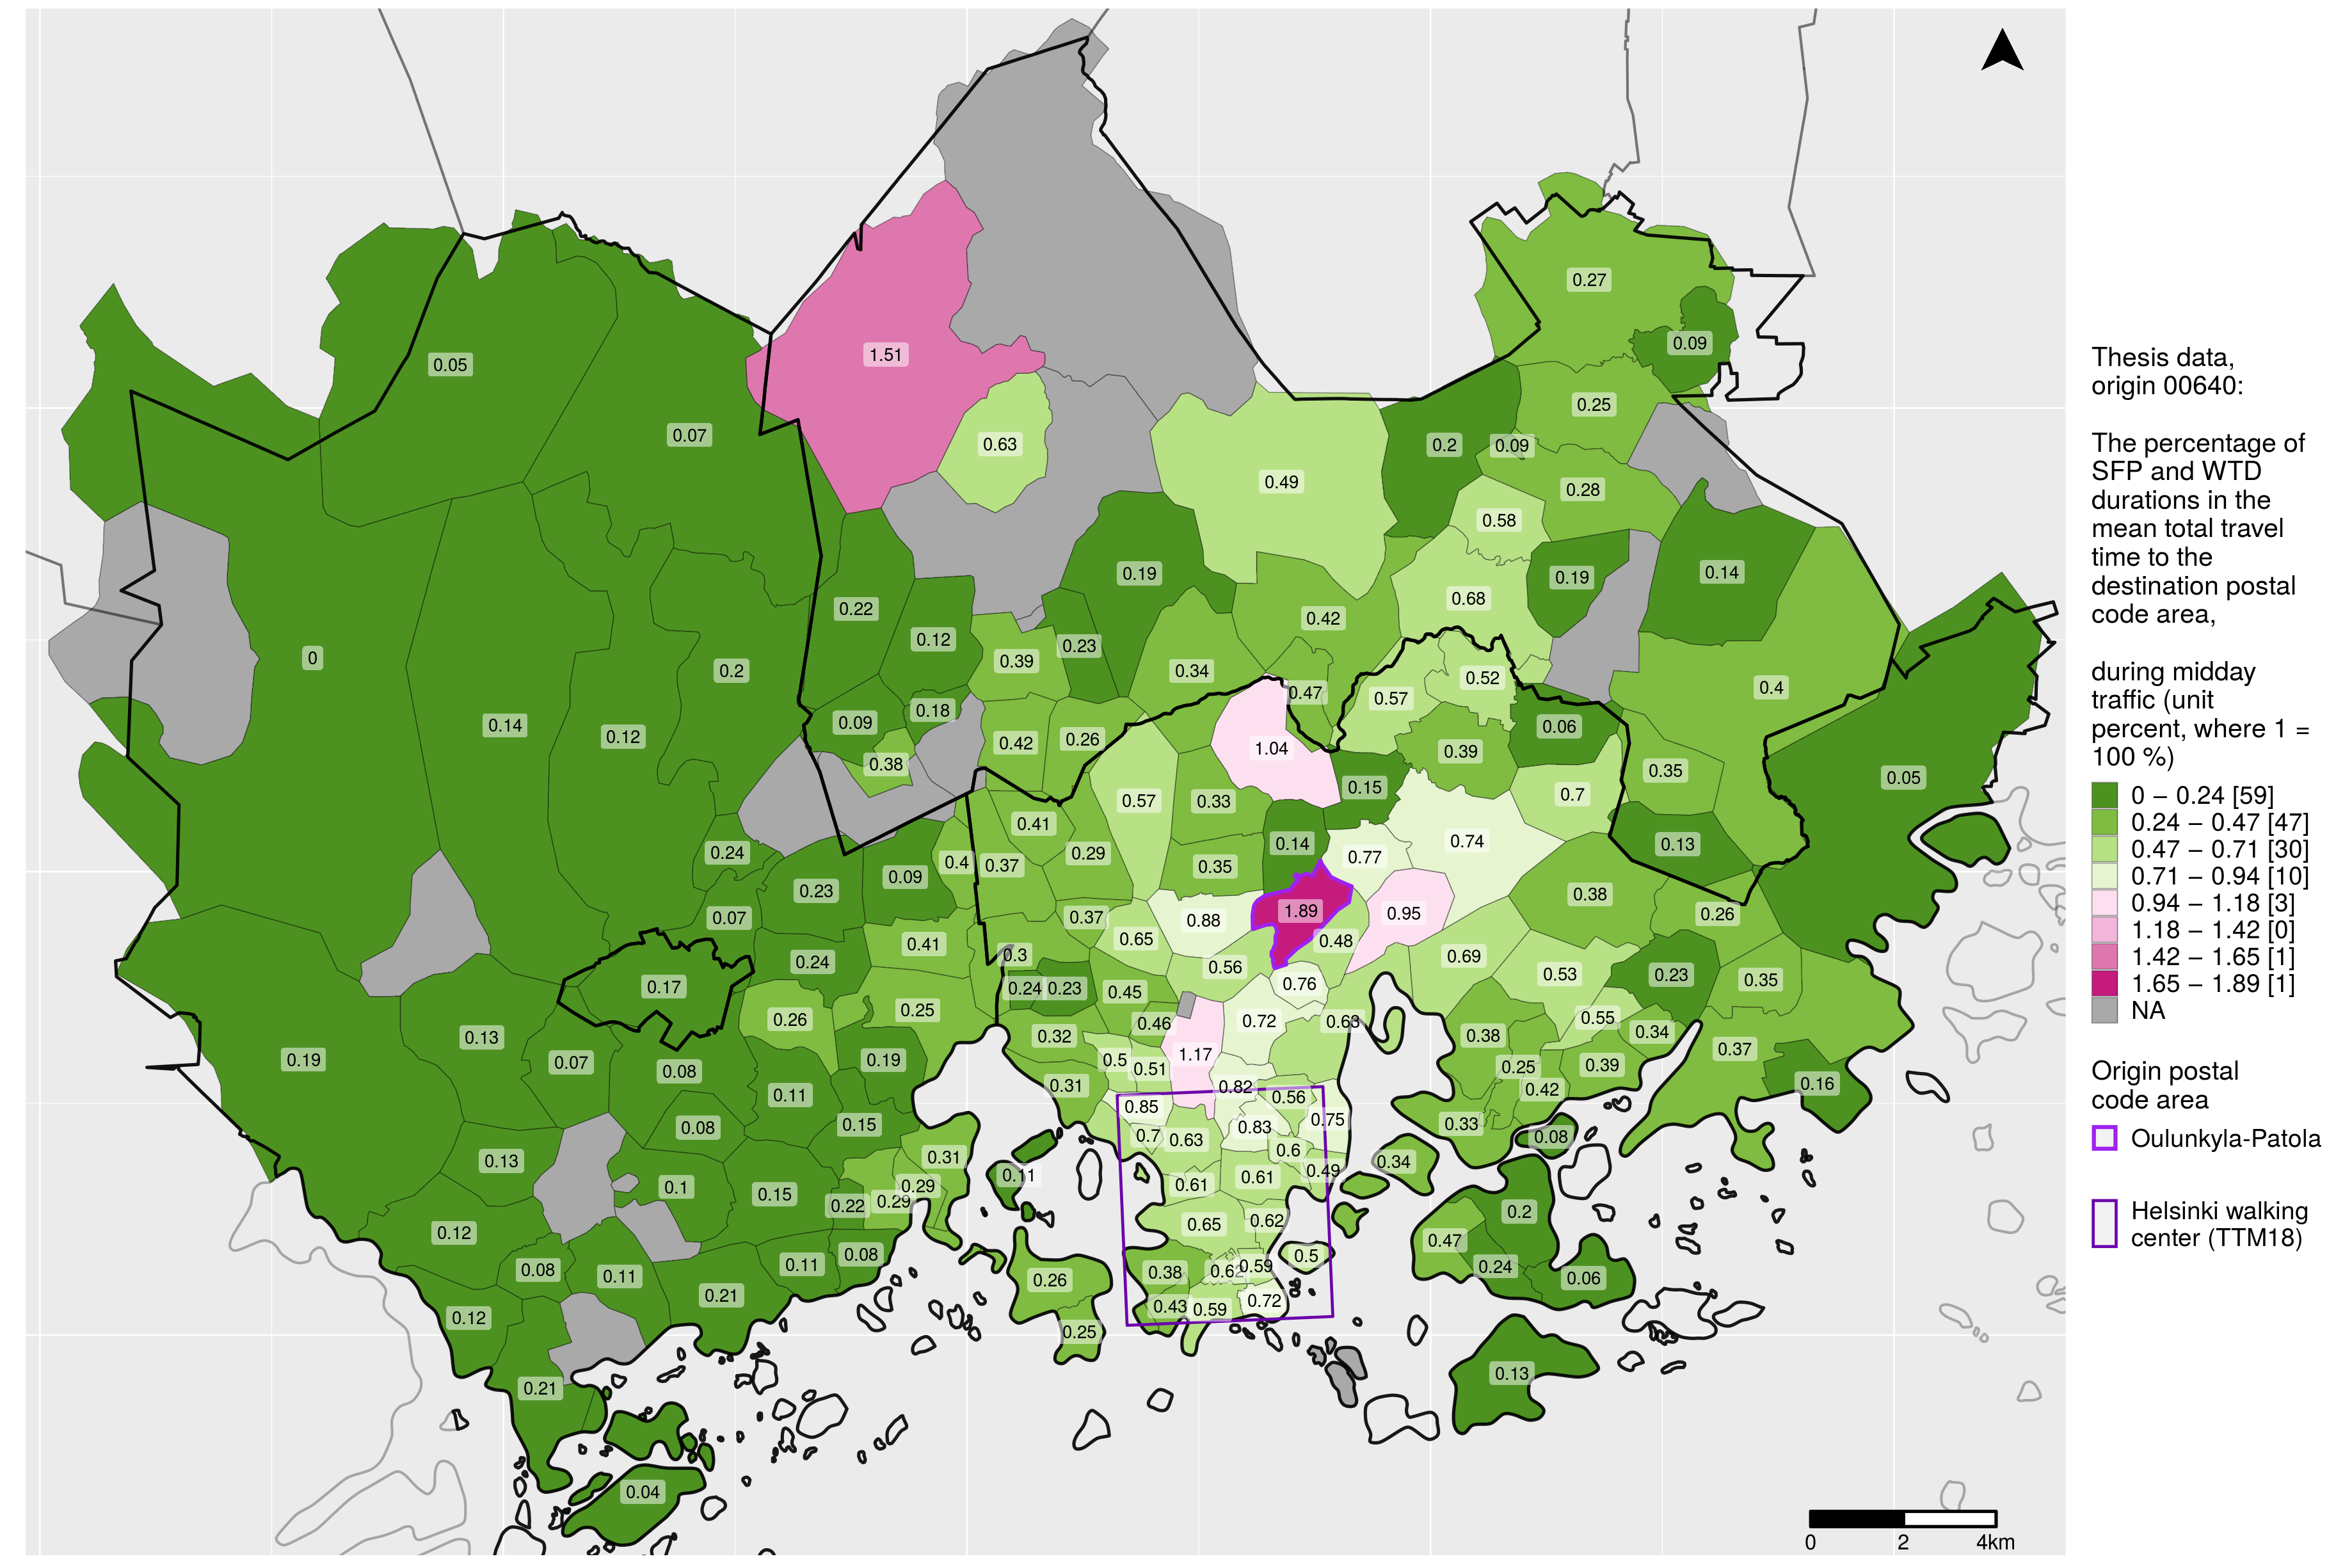
\includegraphics[trim={0.9cm 0.3cm 0.25cm 0.3cm},clip,width=\textwidth]{images/compare_traveltimes_mapfill-msc_m_pct_fromzip-00640_28-09-2020.png}
    \caption[Parking process proportion from Oulunkylä-Patola, midday traffic]{The parking process proportion in the total travel chain, in midday traffic, starting from 00640 Oulunkylä-Patola.}%
    \label{fig:compare_msc_m_pct_00640}%
\end{figure}

\begin{figure}[H]%
    \centering
    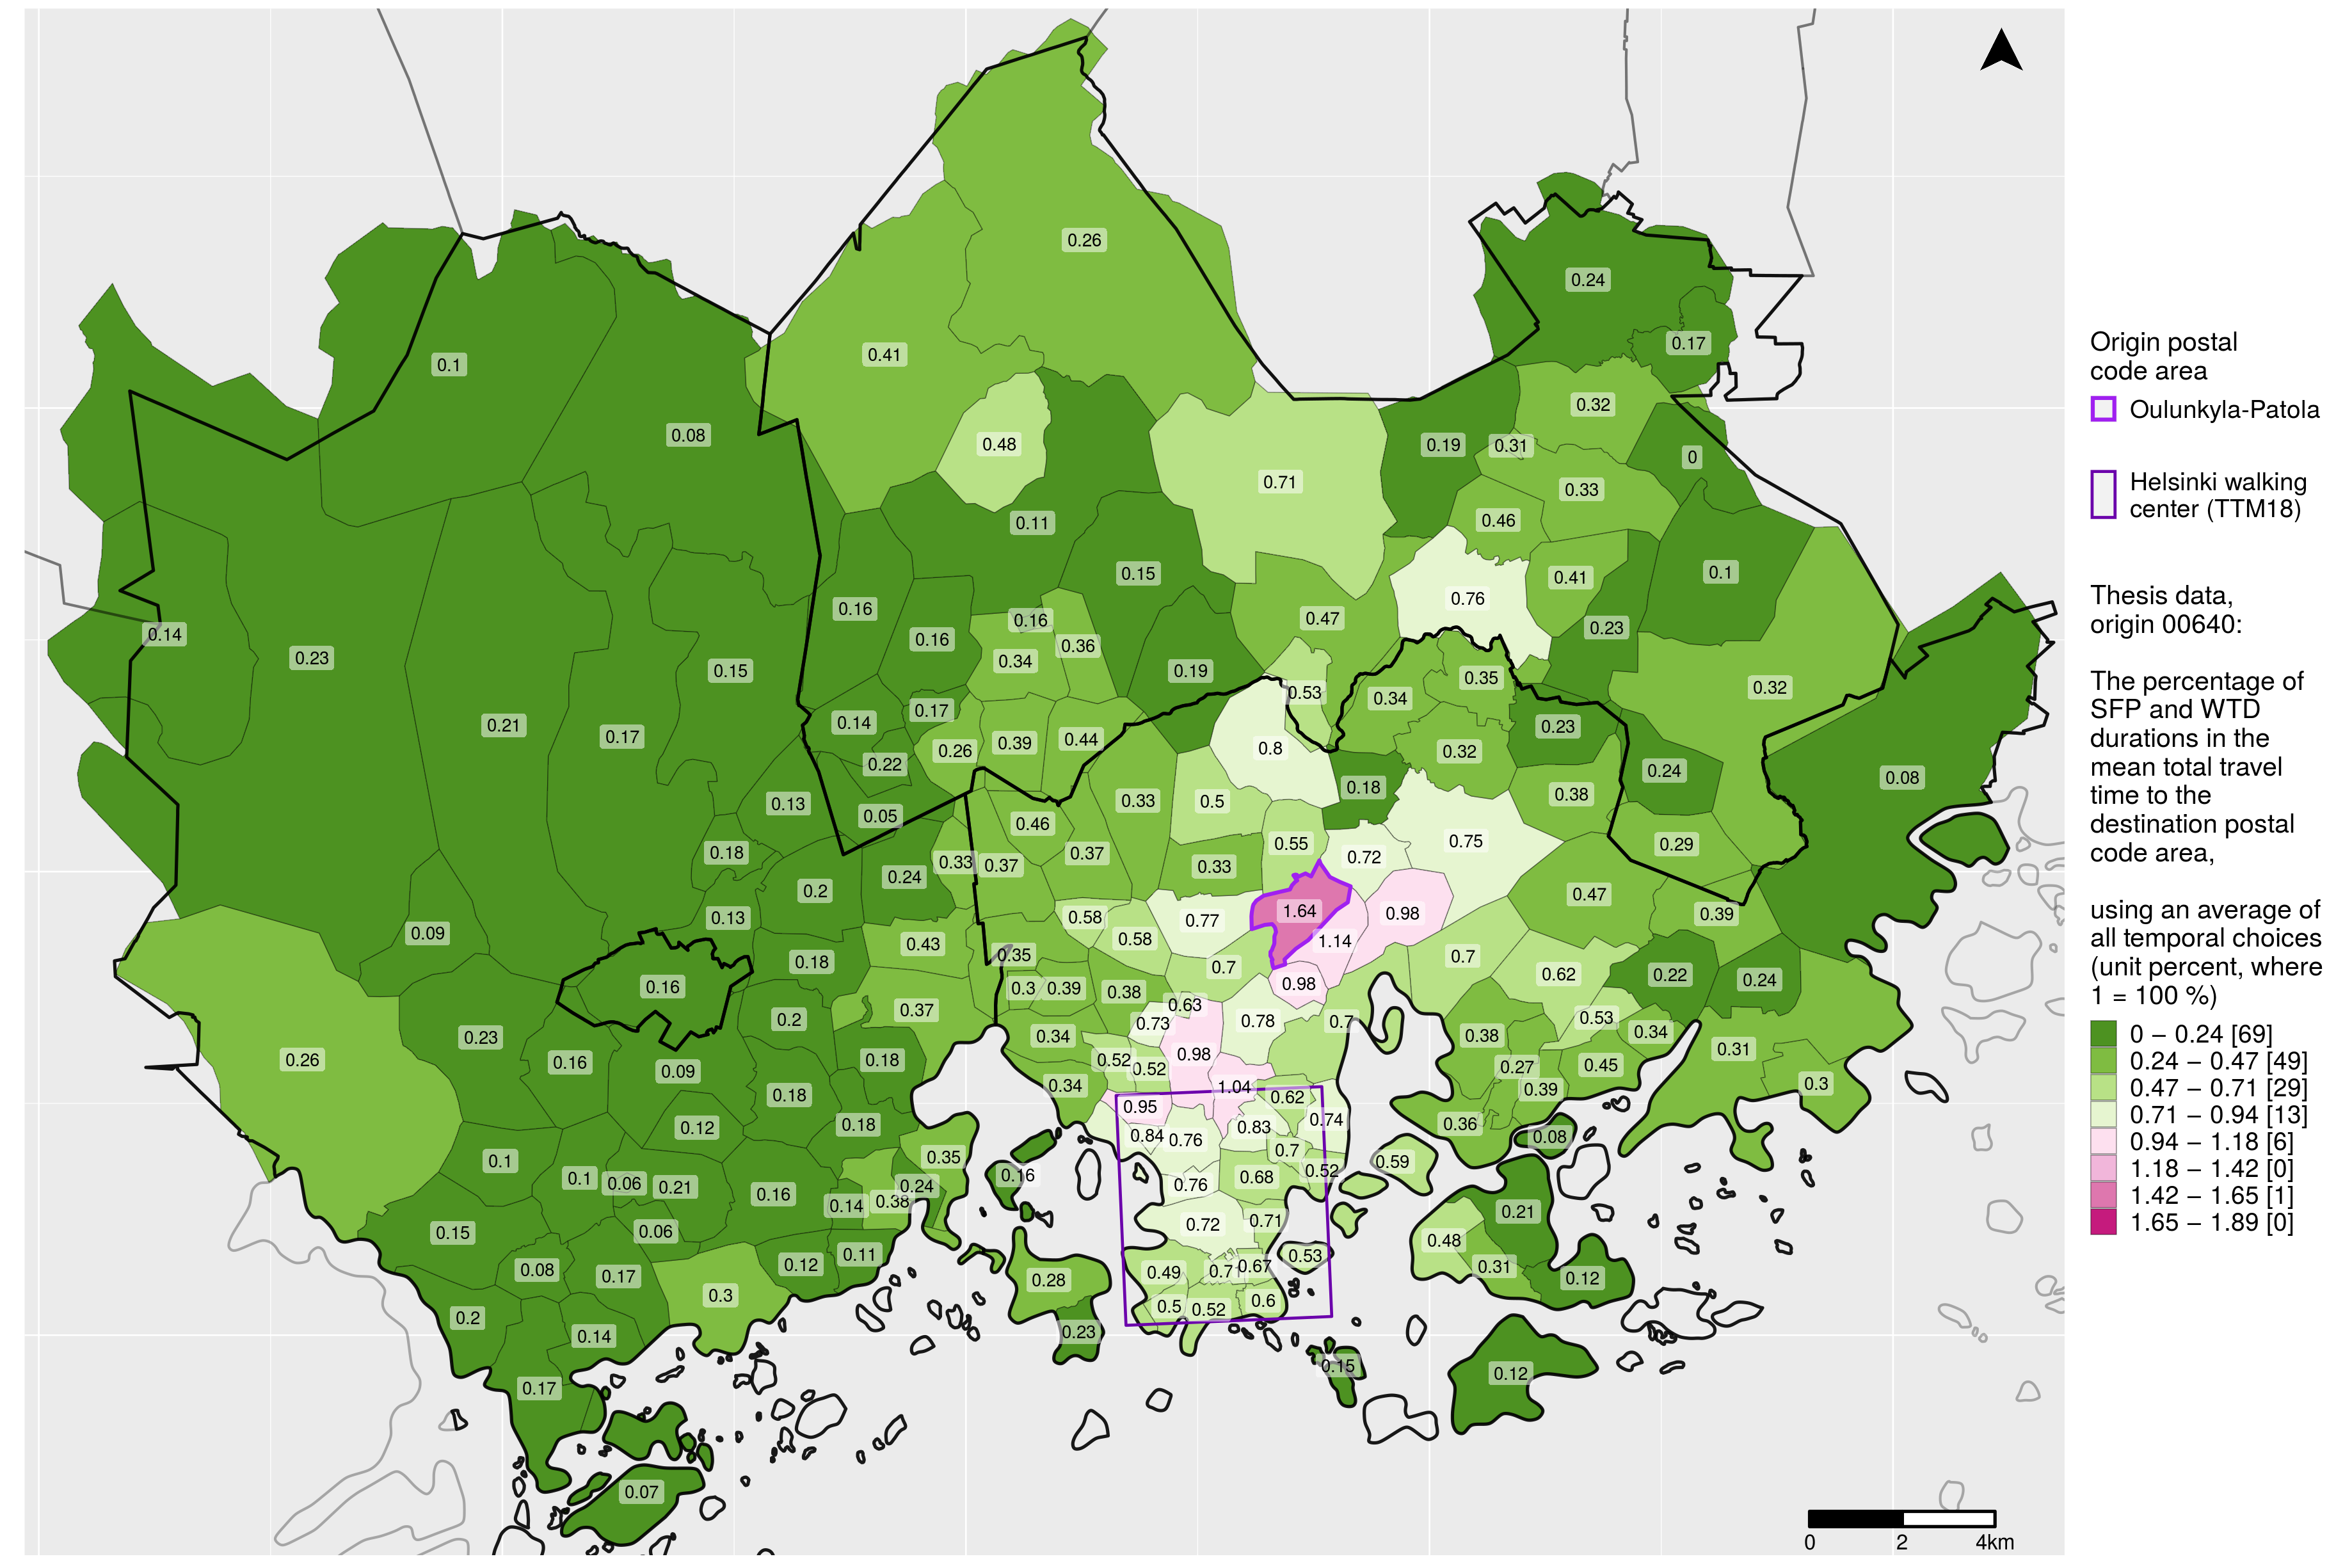
\includegraphics[trim={0.9cm 0.3cm 0.25cm 0.3cm},clip,width=\textwidth]{images/compare_traveltimes_mapfill-msc_all_pct_fromzip-00640_28-09-2020.png}
    \caption[Parking process proportion from Oulunkylä-Patola, all temporal values]{The parking process proportion in the total travel chain, using all temporal values, starting from 00640 Oulunkylä-Patola.}%
    \label{fig:compare_msc_all_pct_00640}%
\end{figure}

The proportion of the parking process in total travel chains starting from 02920 Niipperi, during rush hour traffic, is generally large in all parts of Helsinki Capital Region (figure~\ref{fig:compare_msc_r_pct_02920}). In Espoo, long parking process shares are found from the beltway Ring III postal code areas such as 02780 Kauklahti (42~\%), 02770 Espoon keskus (40 \%), and 02740 Bemböle-Pakankylä (37 \%). In Vantaa, largest shares are found from 01400 Rekola (73 \%), 01530 Veromiehenkylä (54 \%), and 01520 Tammisto (49 \%). Helsinki's largest parking process share is located in 00270 Pohjois-Meilahti (49~\%) with all of the postal code areas of the center of Helsinki reaching lower shares. According to the survey and \textit{TTM} data, the parking process share in a rush hour traffic travel chain from Niipperi to 00160 Katajanokka is a proportionally low 19 percent.

During midday traffic the proportion of the parking process in travel chains starting from the origin postal code area of 02920 Niipperi shows relatively low values (figure~\ref{fig:compare_msc_m_pct_02920}). In fact, the largest parking process share in Espoo is found from the travel chain that starts and ends in Niipperi (67 \%). All other values are equal or below 40 percent. In Helsinki, largest midday traffic parking process shares are found from 00270 Pohjois-Meilahti (47 \%) and 00340 Länsi-Pasila (46 \%) with the center of Helsinki again exhibiting lower parking process values across the board. In Vantaa, large parking process shares were located in 01700 Kivistö (70 \%), 01710 Pähkinärinne (52 \%), and 01680 Askisto (48 \%).

When utilising all available data from the survey and \textit{TTM}, a wholesome picture of the parking process proportion in travel chains from 02920 Niipperi can be gathered (figure~\ref{fig:compare_msc_all_pct_02920}). Many hotspots for large parking process shares may be studied in the different municipalities of Helsinki Capital Region, and no parking process duration is anomalously longer than the total driving segment in any particular travel chain. In Espoo, largest parking process shares are located west from Niipperi, with 02940 Lippajärvi-Järvenperä (44 \%) and 02740 Bemböle-Pakankylä (42 \%) at the top. In Helsinki, northwestern part of the center of Helsinki stands out. Largest shares are located in 00270 Pohjois-Meilahti (52 \%) and in 00290 Meilahden sairaala-alue (48 \%). Vantaa's largest parking process shares were located in 01530 Veromiehenkylä (54 \%) and 01700 Kivistö (52 \%). 

\begin{figure}[H]%
    \centering
    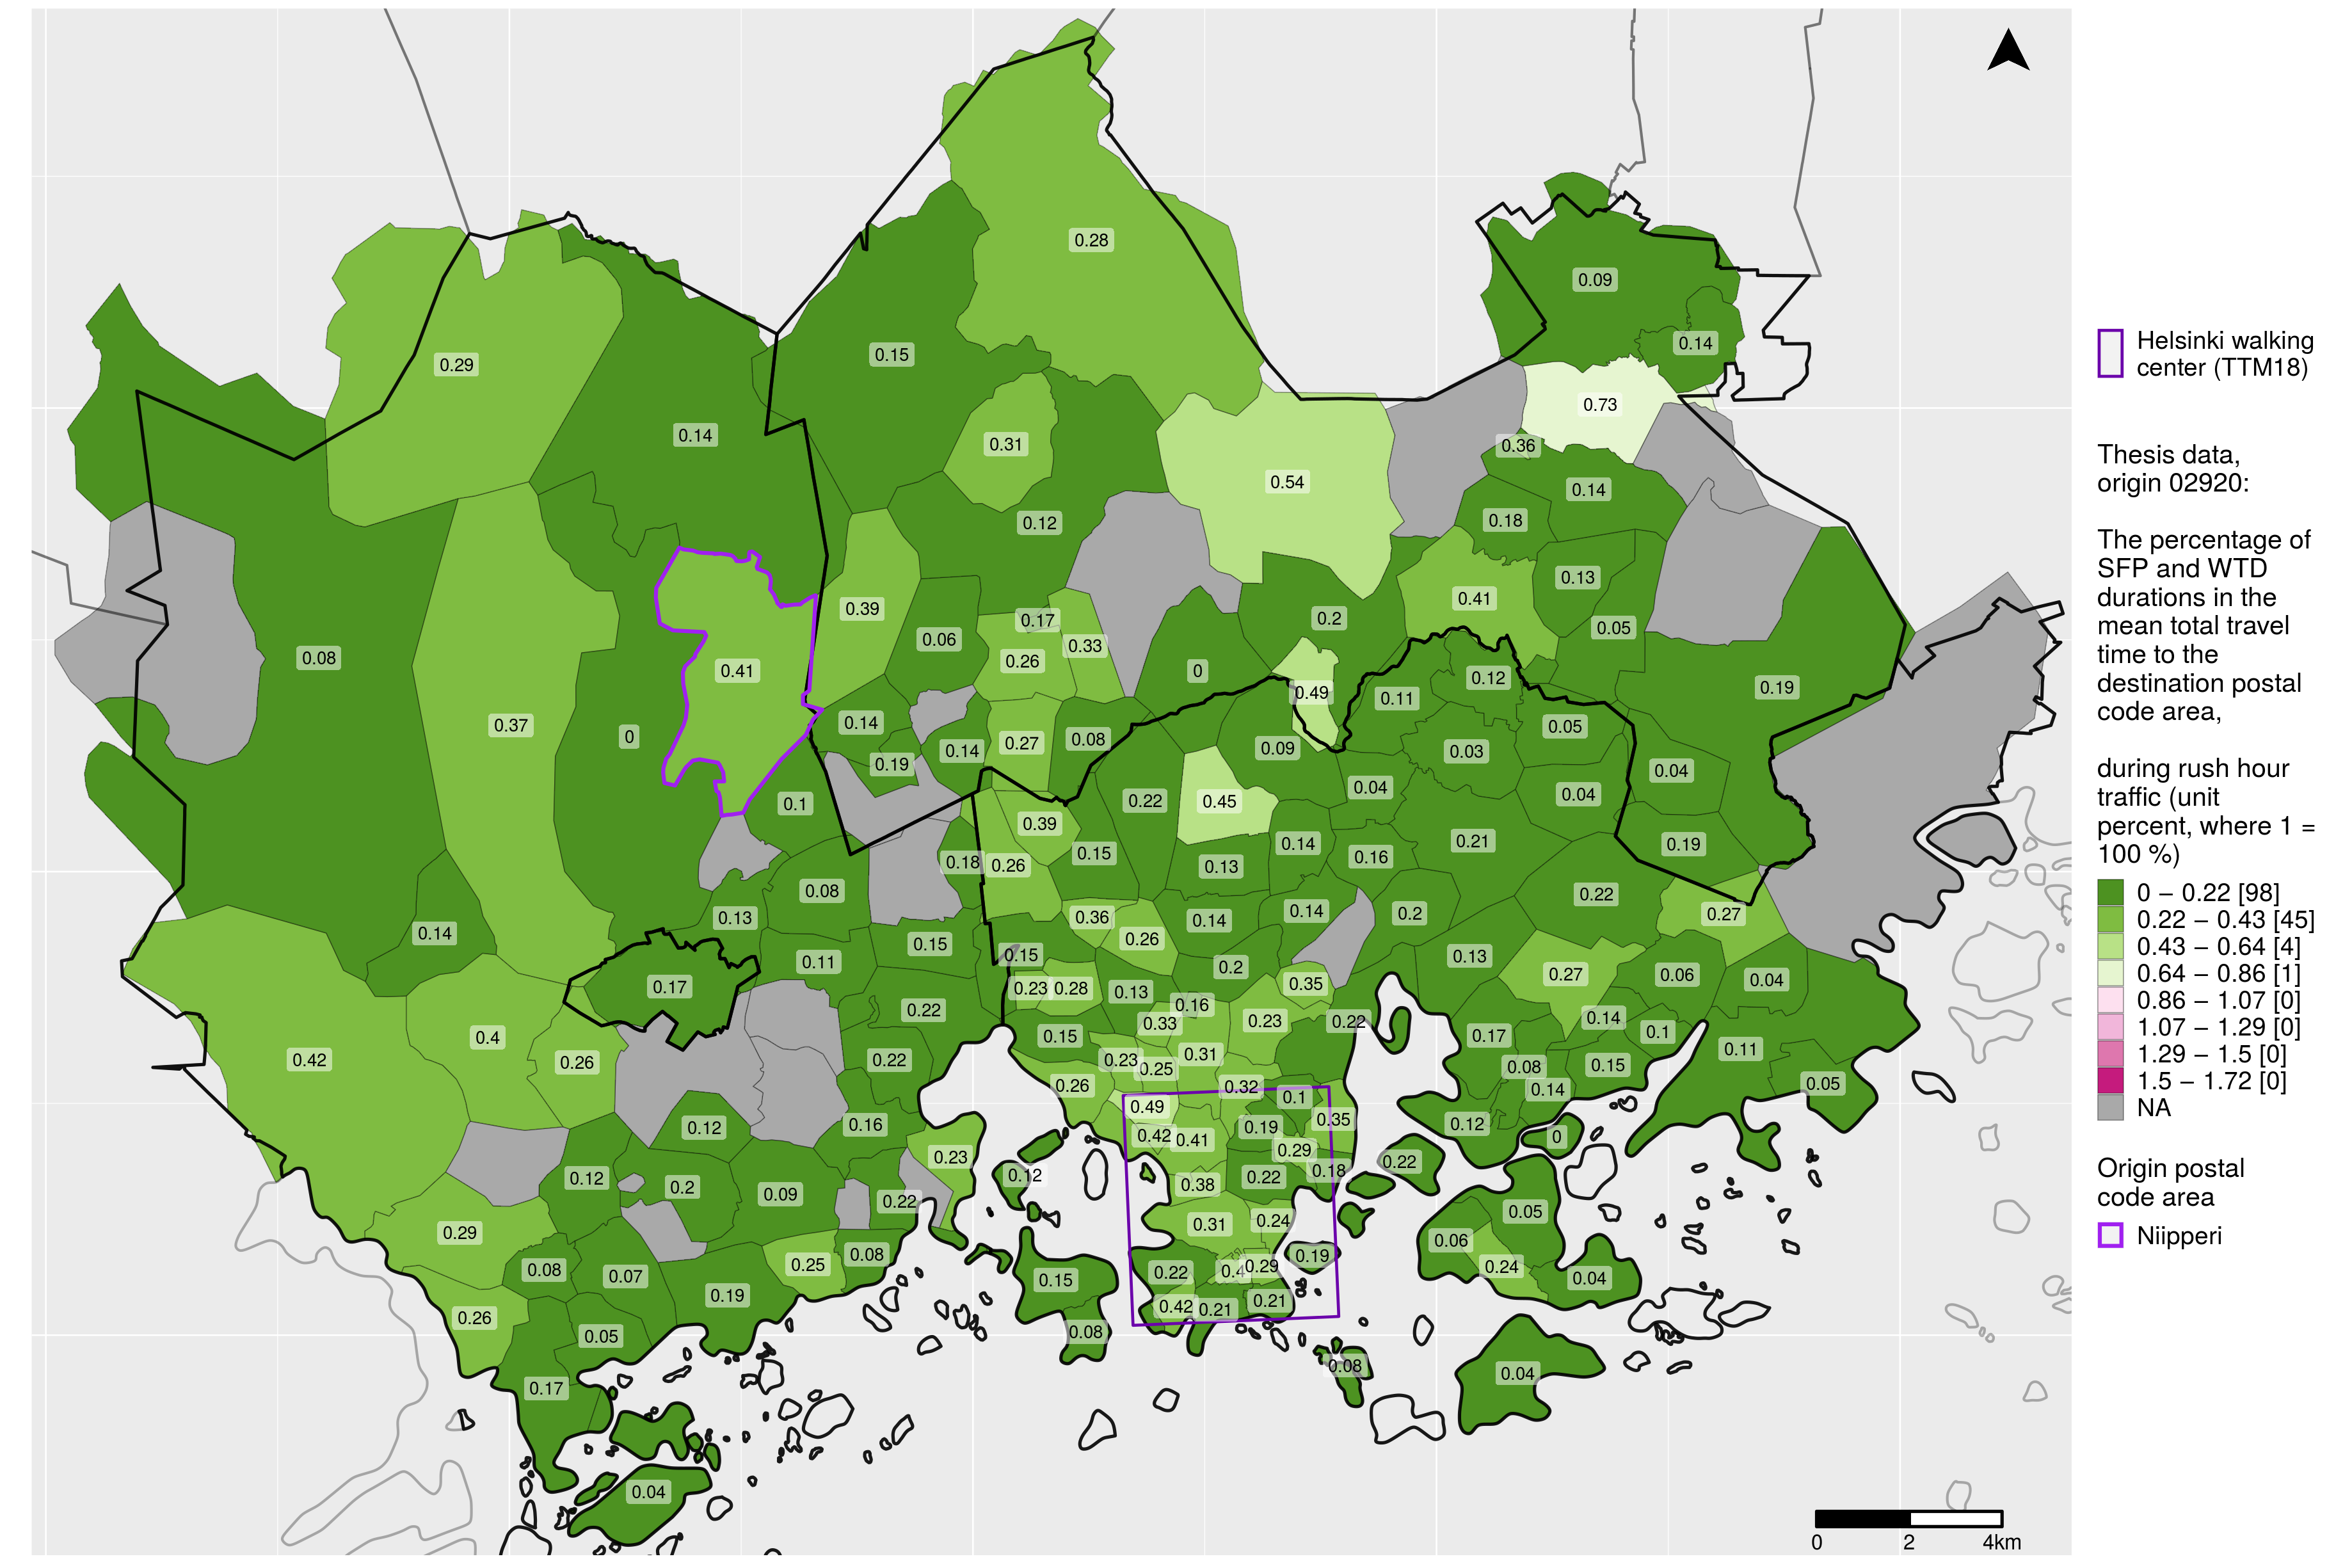
\includegraphics[trim={0.9cm 0.3cm 0.25cm 0.3cm},clip,width=\textwidth]{images/compare_traveltimes_mapfill-msc_r_pct_fromzip-02920_28-09-2020.png}
    \caption[Parking process proportion from Niipperi, rush hour traffic]{The parking process proportion in the total travel chain, in rush hour traffic, starting from 02920 Niipperi.}%
    \label{fig:compare_msc_r_pct_02920}%
\end{figure}

\begin{figure}[H]%
    \centering
    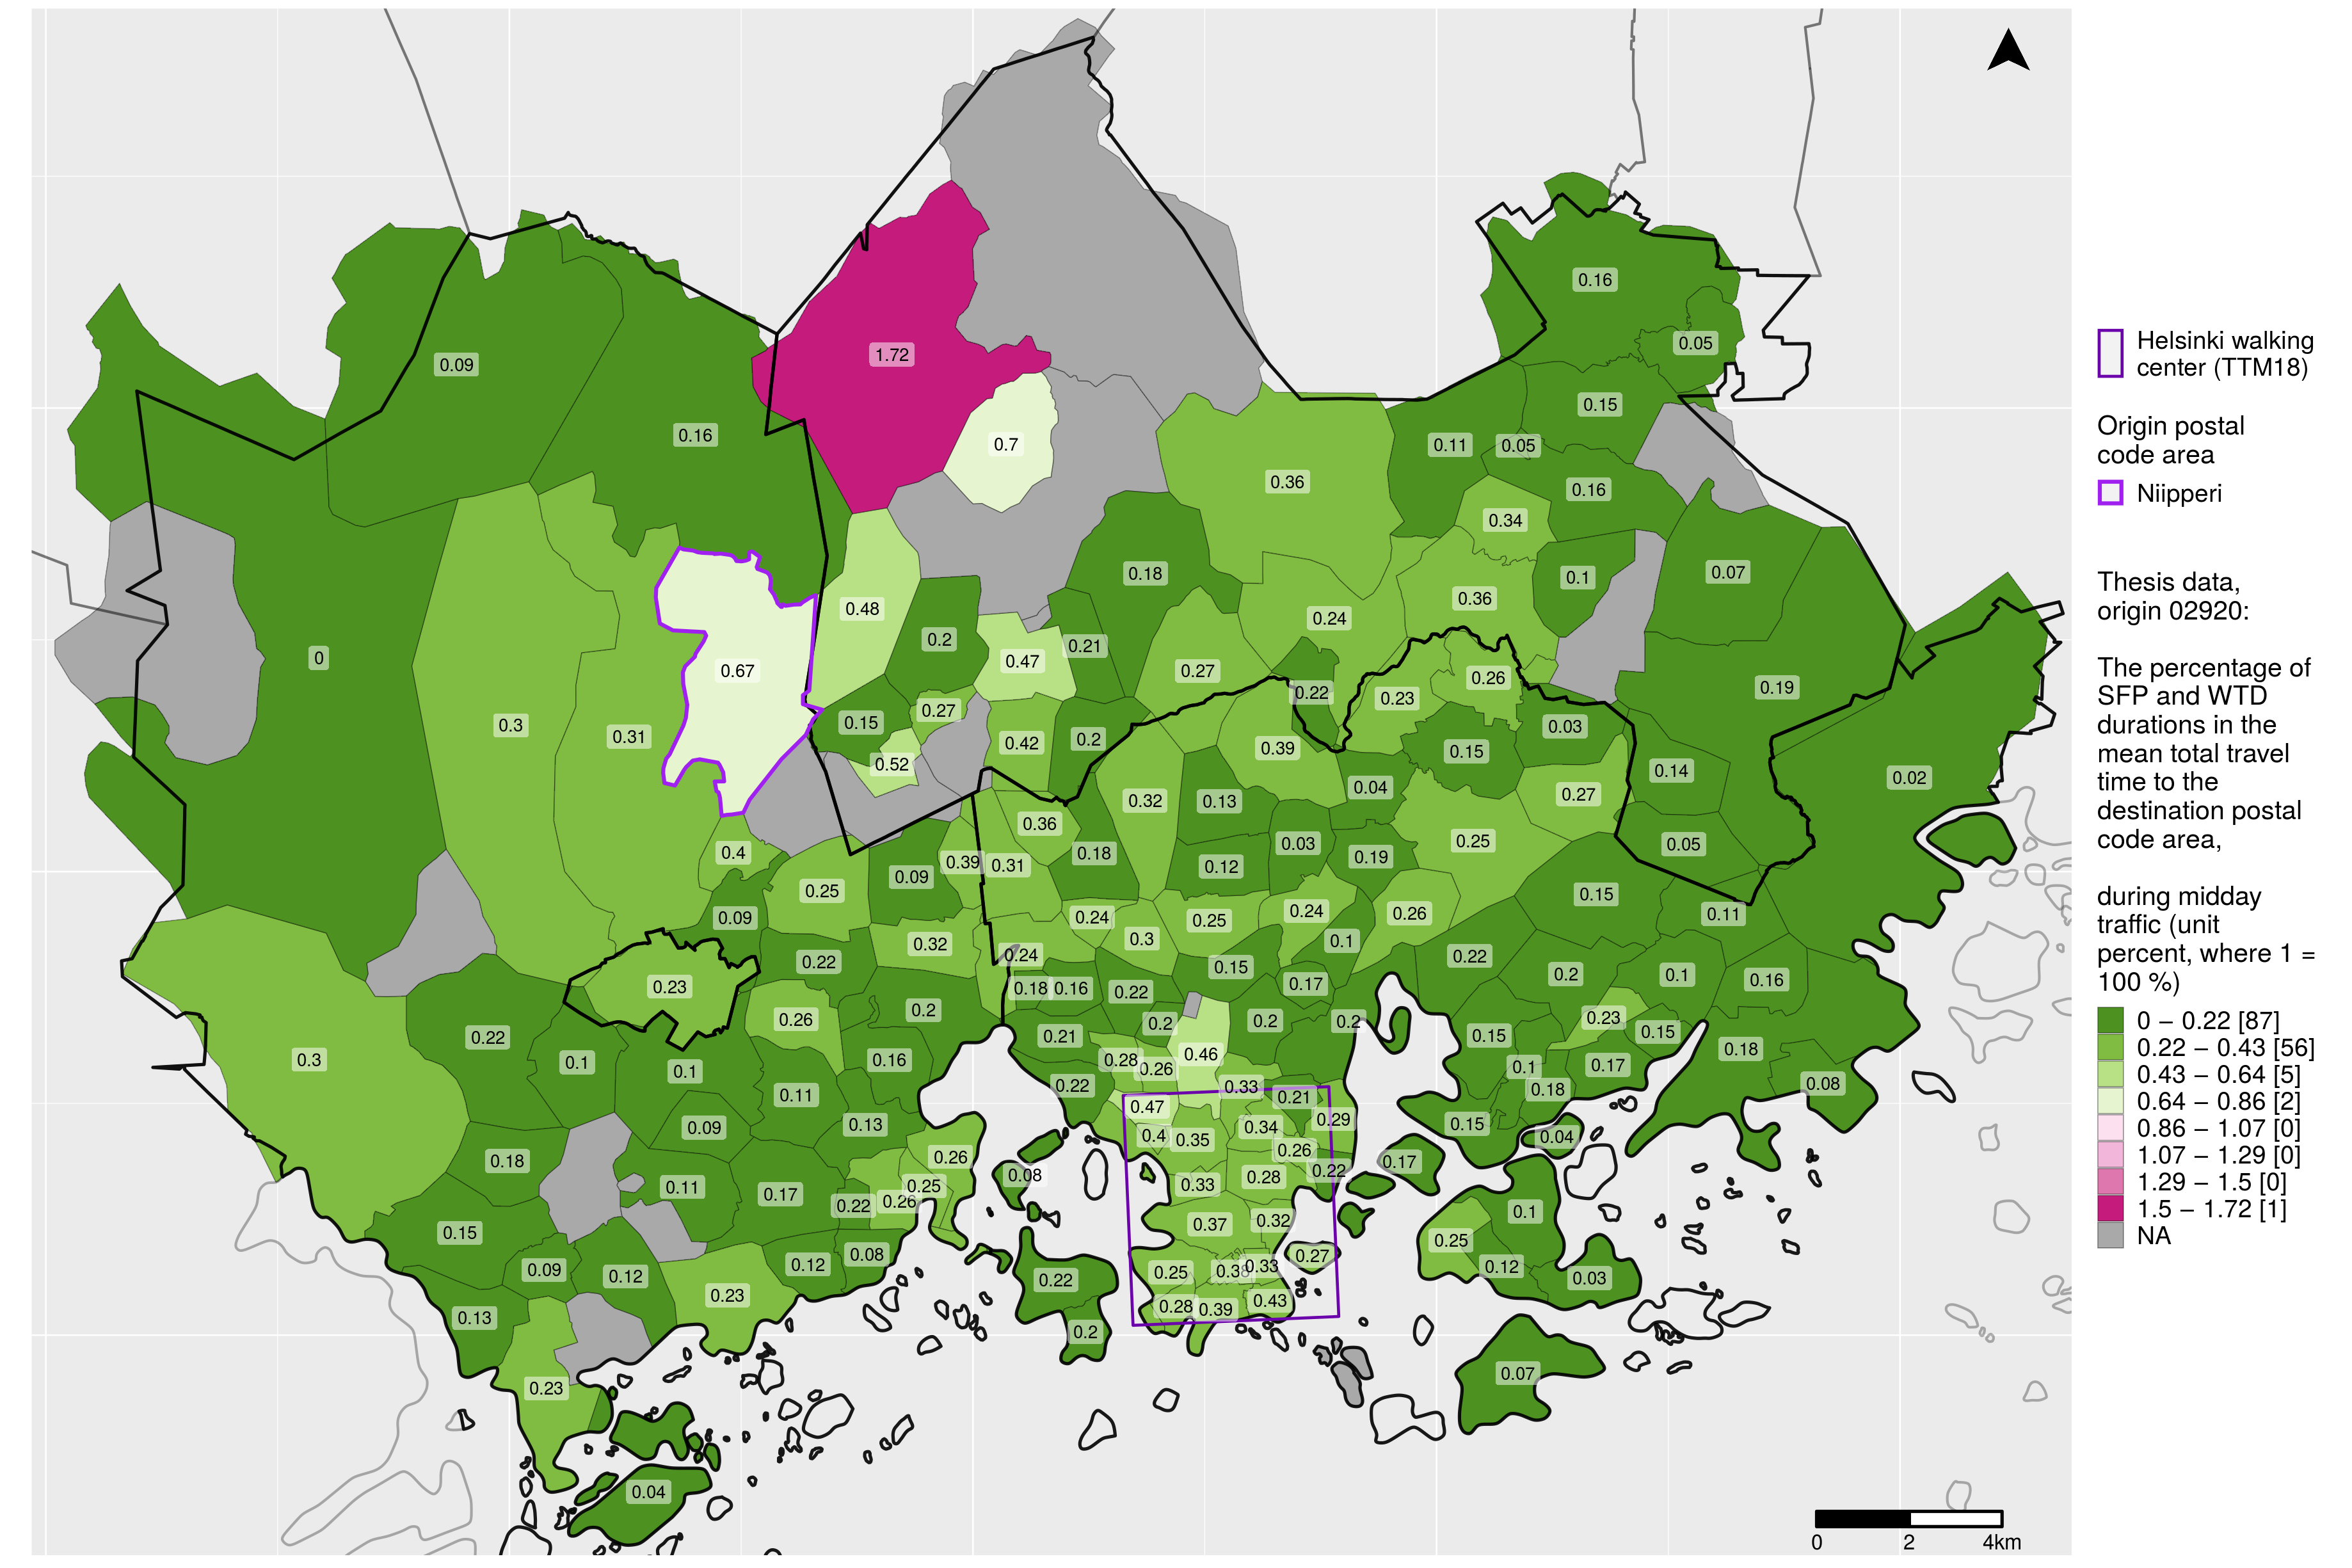
\includegraphics[trim={0.9cm 0.3cm 0.25cm 0.3cm},clip,width=\textwidth]{images/compare_traveltimes_mapfill-msc_m_pct_fromzip-02920_28-09-2020.png}
    \caption[Parking process proportion from Niipperi, midday traffic]{The parking process proportion in the total travel chain, in midday traffic, starting from 02920 Niipperi.}%
    \label{fig:compare_msc_m_pct_02920}%
\end{figure}

\begin{figure}[H]%
    \centering
    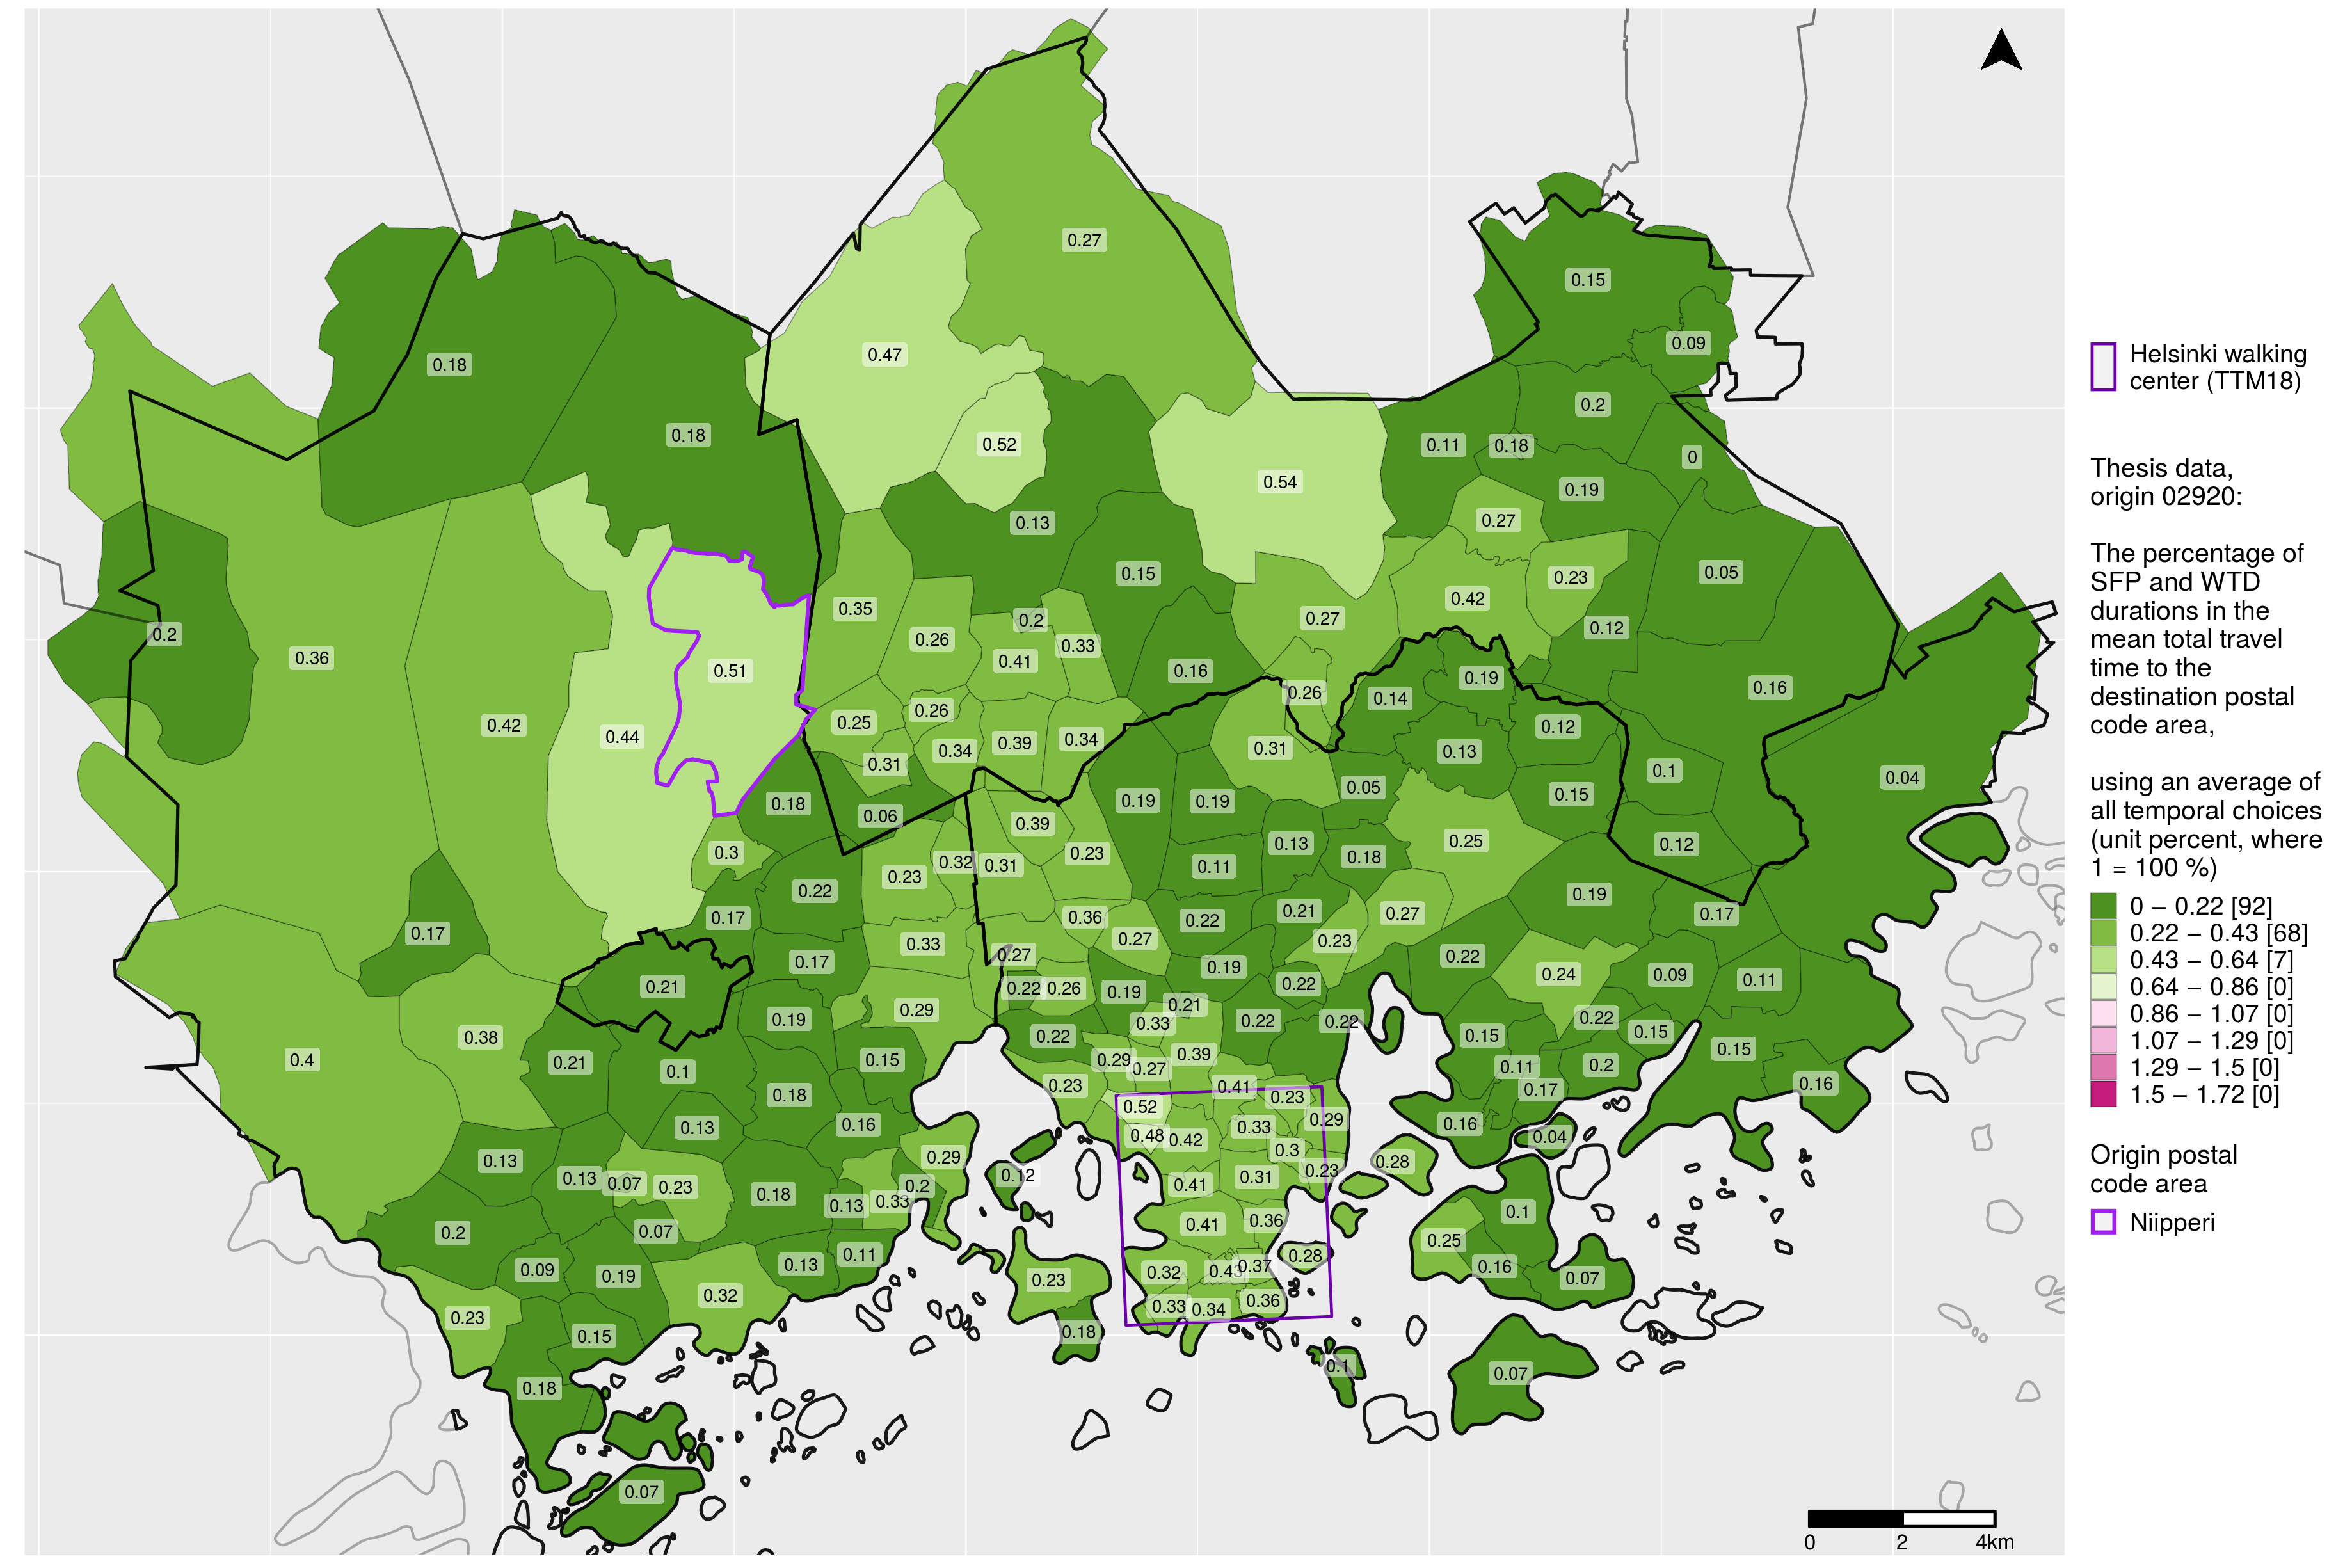
\includegraphics[trim={0.9cm 0.3cm 0.25cm 0.3cm},clip,width=\textwidth]{images/compare_traveltimes_mapfill-msc_all_pct_fromzip-02920_28-09-2020.png}
    \caption[Parking process proportion from Niipperi, all temporal values]{The parking process proportion in the total travel chain, using all temporal values, starting from 02920 Niipperi.}%
    \label{fig:compare_msc_all_pct_02920}%
\end{figure}